\documentclass[11pt]{amsart}
\input{commands.tex}
\usepackage[textsize=tiny]{todonotes}
\title{The topology of algebraic manifolds}
\author{Thomas Brazelton}
\date{Last compiled: \today}
\begin{document}

\begin{abstract}
Course notes from MATH231b: algebraic topology II, taught at Harvard in Spring 2026.
\end{abstract}

\maketitle

\begin{center}
    \url{https://github.com/tbrazel/math231br}
\end{center}


\setcounter{section}{-1}
\section{About}

These notes are from a MATH213BR, a second-semester graduate algebraic topology class with a free-floating curriculum taught at Harvard in spring of 2026. This particular course is modeled off of Hirzebruch's amazing 1962 text \emph{Neue topologische Methoden in der algebraischen Geometrie}. Theorem counters and page references refer to the 1995 reprinting in English \cite{Hirzebruch}.

\subsection{Overview}

\textbf{Part 1}: We begin with the theory of sheaves of sets and discrete groups on topological spaces, developing their cohomology and comparing it with singular and de Rham cohomology. We continue with fiber bundles and develop their basic theory. We then discuss vector bundle theory and Chern and Pontryagin classes. 

\textbf{Part 2}: We discuss oriented and complex cobordism, genera, the $L$-genus and Todd genus, and the index of a $4n$-manifold. We prove Hirzebruch's signature theorem as well as Riemann-Roch for algebraic manifolds.

\setcounter{tocdepth}{1}
\tableofcontents{}

\subsection{References}
Aside from the main text, which we deviate from at various points, some other references which have informed the presentation here include:
\begin{itemize}
    \item \emph{sheaf theory}: Godement's original work \cite{godementTopologieAlgebriqueTheorie1958}, and of course Serre's \cite{FAC}
    \item \emph{fiber bundles}: Steenrod's 1951 printing \cite{Steenrod-fibre-bundles}
    \item \emph{K\"{a}hler manifolds}: Michael Wong's 2013 \href{https://wiki.epfl.ch/kaehler2013/notesexercises}{course notes}
    \item \emph{cobordism}: Dan Freed's notes \cite{Freed-bordism} and Haynes Miller's notes \cite{millerNotesCobordism}
    \item \emph{genera}: Hirzebruch's book \cite{MMF}
    \item \emph{complex manifolds}: Griffiths and Harris \cite{griffithsPrinciplesAlgebraicGeometry1978}
\end{itemize}

\subsection{Acknowledgements}

Thank you to Zo\"{e} Batterman, Vincent Costa, Frank Gubars, Grayson Kemplin, Luke Lelli, Gabe Ong, Brian Siew, and Greg Wong for offering suggestions and changes to the notes. Thanks to Gage Martin and Sidhanth Raman for helpful conversations in preparing this class.

\section{Sheaves}

The definition of a \emph{sheaf} in Hirzebruch is perhaps a bit different from what we're used to. He wants to think of sheaves as \emph{living over} a space $X$, whereas we might be comfortable thinking about sheaves as local data across a space. We'll see how these perspectives are equivalent.

\begin{definition}\label{def:sheaf} 
A \emph{sheaf of abelian groups} over a topological space $X$ is a topological space $S$ with the data of a surjective continuous map $\pi \colon S \to X$, for which
\begin{itemize}
    \item $\pi$ is a \emph{local homeomorphism}, meaning for every point $s\in S$ there is an open neighborhood $U\ni s$ for which
    \begin{align*}
        \pi_{|U} \colon U \to \pi(U)
    \end{align*}
    is a homeomorphism
    \item for every $x\in X$, the \emph{stalk} $S_x := \pi^{-1}(x)$ has the structure of an \emph{abelian group}
    \item the abelian group structure on $S_x$ is \emph{continuous in $x$}. Precisely, forming inverses in each fiber defines a continuous function:
    \begin{align*}
        S &\to S \\
        s &\mapsto -s,
    \end{align*}    
and if we denote by $S \times_X S$ the subspace
    \begin{align*}
        S \times_X S := \left\{ (s_1,s_2) \in S \times S \colon \pi(s_1)=\pi(s_2) \right\} \subseteq S \times S,
    \end{align*}
    then the operation of addition is a continuous function:
    \begin{align*}
        S \times_X S &\to S \\
        \left( (\alpha,x), (\beta,x) \right) &\mapsto (\alpha + \beta,x).
    \end{align*}
\end{itemize}
\end{definition}

We should think about a sheaf of abelian groups as being a space where we can do abelian group operations (addition, subtraction), but where the abelian group in which we're working is \emph{changing} according to the topology of $X$.

\begin{example}[Zero sheaf] The identity map $X \to X$ can be considered a sheaf, where the abelian group structure on each stalk is just the trivial group with one element.
\end{example}


\begin{example}[Constant sheaves]
\label{exa:constant-sheaf-espace-etale}
For any abelian group $A$ and any space $X$, we get a \emph{constant sheaf}
\begin{align*}
    X \times A \to X,
\end{align*}
where $\pi$ is the projection onto $X$. When $A = \left\{ 0 \right\}$, this recovers the zero sheaf above.
\end{example}

\begin{example}[Skyscraper sheaves]
\label{exa:skyscraper-sheaves}
If we want build a sheaf with some \emph{prescribed} fiber $A$ over a point $x\in X$ (we want a name for the map of the inclusion of a point, so let's call it $i \colon \{x\} \to X$), we have an nice way to do this -- namely, we can take the discrete set underlying the abelian group $A$, and build the space which we call $i_\ast A$, defined as
\begin{align*}
    i_\ast A = \frac{X \times A}{(y,a_1)\sim (y,a_2)\text{ for }y\ne x}.
\end{align*}
That is, we identify all the points of $A$ together over every point in $X$ \emph{except} our specified point $x$. We call it a \emph{skyscraper sheaf} because it has this big tall stalk at $x$ and is flat everywhere else. This space comes equipped with a projection back to $X$ which is a continuous local homeomorphism, and the abelian group structure on the stalks over points other than $x$ are just the structure on the one-element group. Note that this resulting space $i_\ast A$ is very much not Hausdorff.
\end{example}


\begin{example}[{c.f.~\cite[1.3]{Bredon-sheaf}}] The \emph{line with doubled origin} is the skyscraper sheaf over $\R$ defined by $i_\ast (\Z/2)$, where $i \colon \{0\}\hookto \R$ is the inclusion of the origin.
\end{example}


\begin{notation} For any sheaf of abelian groups $\pi \colon S \to X$, we have the so-called \emph{zero section} $z \colon X \to S$, sending each element $x\in X$ to the zero element in $S_x$. This map is continuous and has the property that
\begin{align*}
    \pi\circ z = \id_X.
\end{align*}
\end{notation}

\begin{exercise}\label{exer:image-zero-section-is-open}
Let $\pi \colon X \to S$ be any sheaf and $z \colon X \to S$ the zero section. Then $\im(z) \subseteq S$ is open.
\end{exercise}


\begin{example} The projection $\R \to S^1$ cannot be given the structure of a sheaf of abelian groups.
\end{example}
\begin{proof} We're tempted to say it looks like a sheaf, since each fiber looks like $\Z$, however it turns out there is no way to endow these fibers simultaneously with the additive structure of the integers. Suppose towards a contradiction there was. Then composing with the zero section, we get a composite which is the identity:
\begin{align*}
    S^1 \xto{z} \R \xto{\pi} S^1.
\end{align*}
Applying $\pi_1$ or $H_1$ for instance, we have that the identity on $\Z$ factors through zero, which is a contradiction.
\end{proof}

\begin{remark} Just as we have a sheaf of abelian groups, we can have a sheaf with other structures as well --- we could have a sheaf of $R$-modules for instance. All that's important is that:
\begin{enumerate}
    \item our structure is a set with extra data
    \item we have that data in every stalk
    \item the data varies continuously in the stalks
\end{enumerate}
\end{remark}

\begin{definition} A \emph{morphism of sheaves} between $\pi \colon S\to X$ and $\til{\pi} \colon \til{S} \to X$ is a continuous map $f \colon S \to \til{S}$ satisfying the following properties:
\begin{itemize}
    \item $\til{\pi}\circ f = \pi$, that is, we have a commutative diagram
\[ \begin{tikzcd}
    S\ar[dr,"\pi" below left]\ar[rr,"f"] &  & \til{S}\ar[dl,"\til{\pi}" below right]\\
     & X & 
\end{tikzcd} \]
    Note this implies that $f$ restricts to a map on each stalk, that is, we get maps $f_x \colon S_x \to \til{S}_x$ for each $x\in X$
    \item for each $x\in X$, the induced map on stalks
    \begin{align*}
        f_x \colon S_x \to \til{S}_x
    \end{align*}
    is an abelian group homomorphism.
\end{itemize}
\end{definition}

\begin{exercise} Show that every morphism between sheaves of abelian groups is a local homeomorphism.
\end{exercise}

% The opposite of the zero section, in some sense, is a section which is nowhere zero.
% \begin{definition} A \emph{nonvanishing global section} of a sheaf $\pi \colon S \to X$ is a section $s \colon X \to E$.....\todo{need a point to this. can we say anything interesting about the existence or non-existence of nonvanishing global sections? I want to use the existence of one to make an isomorphism with another sheaf. idk how to do this immediately though}
% \end{definition}


\begin{definition}\label{def:injective-surjective-mononomorphism-of-sheaves} 
We say a morphism of sheaves $f \colon S \to \til{S}$ is:
\begin{enumerate}
    \item \emph{injective} if each $f_x$ is injective
    \item \textit{surjective} if each $f_x$ is surjective.
\end{enumerate}
We say a sequence of maps of sheaves
\begin{align*}
    S \xto{f} T \xto{g} U
\end{align*}
is \emph{short exact} if $S_x \xto{f_x} T_x \xto{g_x} U_x$ is a short exact sequence of abelian groups for every $x\in X$.
\end{definition}

\subsection{Sheaves and presheaves}

Given any sheaf $S\to X$, we can ask when we have \emph{sections}, which are maps $X \to S$ that are right inverses to the projection map $\pi$.

\begin{definition} We define the set of \emph{sections} by
\begin{align*}
    \Gamma(X,S) := \left\{ s \colon X \to S \text{ continuous} \mid \pi\circ s = \id_X \right\}.
\end{align*}
Note that $\Gamma(X,S)$ is an abelian group by adding sections pointwise. The zero element of $\Gamma(X,S)$ is the zero section.
\end{definition}

Note that we don't need sections to be defined on all of $X$ --- we could look at sections defined on subspaces. For instance if $U \subseteq X$ is an open subspace, we can define
\begin{align*}
    \Gamma(U,S) := \left\{ s \colon U \to S \mid \pi\circ s = \id_U \right\}.
\end{align*}
%
If $V \subseteq U$ is an open subspace, there is a natural \emph{restriction} map
\begin{align*}
    \res_V^U \colon \Gamma(U,S) &\to \Gamma(V,S) \\
    s &\mapsto s_{|V}.
\end{align*}
%
\begin{notation} For $X$ a topological space, we denote by $\Open(X)$ the category whose objects are open subspaces of $X$ and whose morphisms are inclusions. Then the constructions above tell us that $\Gamma(-,S)$ defines a functor
\begin{align*}
    \Gamma(-,S) \colon \Open(X)^\op \to \Ab.
\end{align*}
This is called the \emph{presheaf} associated to $S$.
\end{notation}

\begin{terminology} If $S \to X$ is a sheaf, an element of $\Gamma(X,S)$ will be called a \emph{global section}. This is to indicate it is defined globally, i.e. everywhere on $X$, in contrast with sections only defined locally on some open subspace $U$.
\end{terminology}

Let's think about what structures of $S$ we can recover from its presheaf.

\begin{question} Can we recover the stalk $S_x$ from the presheaf $\Gamma(-,S)$?
\end{question}

We can't just take $\Gamma$ and evaluate it on the one-point set $\left\{ x \right\}$ since this won't be open in most reasonable topological spaces. Instead, we can take elements in $\Gamma(U,S)$ for any $U \ni x$, and glue sections together along restriction of open sets containing $x$. This is called a \emph{colimit} (in classical terminology, a \emph{direct limit}):
\begin{align*}
    \colim_{U\ni s}\Gamma(U,S).
\end{align*}
%
\begin{proposition}\label{prop:colimit-sections-is-stalk}
For every sheaf of abelian groups $S \to X$ and every $x\in X$, the canonical ``evaluation at $x$'' map
\begin{align*}
    \ev_x \colon \colim_{U\ni s} \Gamma(U,S) \to S_x
\end{align*}
is an isomorphism of abelian groups.
\end{proposition}
\begin{proof} If $s_1(x) = s_2(x) = a$, then since $\pi$ is a local homeomorphism, there is some small neighborhood $V \ni a$ on which $\pi_{|V} \colon V \to \pi(V)$ is a local homeomorphism. In particular since $s_{1|\pi(V)}$ and $s_{2|\pi(V)}$ are both sections (right inverses) of $\pi_{|V}$ they must agree. Since they agree on a sufficiently small open neighborhood around $x$, they agree in the colimit. This establishes injectivity.

To see surjectivity, if $a\in S_x$, we want to create a section $s$ defined in a neighborhood $U$ of $x$ for which $s(x) = a$. We again leverage the fact that $\pi$ is a local homeomorphism to find some neighborhood $V \ni a$ for which $\pi \colon V \xto{\sim} \pi(V)$ is a homeomorphism. Then the inverse to this map satisfies $\pi^{-1}(x) = a$.
\end{proof}
This gives us an alternative way to look at stalks. Now we know we can recover stalks from the underlying presheaf.

\begin{question}\label{ques:recover-sheaf-from-presheaf} 
Can we recover the sheaf $S$ from the presheaf $\Gamma(-,S)$?
\end{question}

That is, suppose someone hands you a functor
\begin{align*}
    F \colon \Open(X)^\op \to \Ab,
\end{align*}
and tells you it is of the form $\Gamma(-,S)$ for some sheaf $S$, but they don't tell you what $S$ is. Can you rebuild $S$? Let's denote by
\begin{align*}
    F_x := \colim_{U\ni x} F(U)
\end{align*}
the stalk at a point $x\in X$. Then we know how to construct the sheaf as a \emph{set}, namely it is
\begin{align*}
    \amalg_{x\in X} F_x \to X.
\end{align*}
The question then becomes how to topologize the thing on the left. Each $F_x$ has the discrete topology as an abelian group, and the disjoint union has the discrete topology a priori -- but if we accept this topology, then in general we won't have the property that the projection map is a local homeomorphism. So we need to hunt for a different topological structure. The trick to finding it is that we know how to write down sections, and we want to \emph{force sections to be continuous}.

We denote by
\begin{align*}
    \germ_x \colon F(U) \to F_x
\end{align*}
the structure map (part of the data of the colimit) to the stalk (c.f.~\Cref{prop:colimit-sections-is-stalk}; we called this an evaluation map earlier when we knew $F(U)$ was comprised of actual sections. We don't know that a priori now). For any $s\in F(U)$, we then get a composite
\begin{align*}
    U &\to \amalg_x F_x \\
    x &\mapsto \germ_x(s).
\end{align*}
This should be like a section of the sheaf, so we want it to be continuous. We want the preimage of opens to be open, and since $U$ is indeed open, an easy way to try to force continuity is to ask for the image of this map above to be open.

\begin{definition}\label{def:basis-for-topology-on-espace-etale} 
We define a \emph{basis}\footnote{See \cite[II\S13]{Munkres} if this is an unfamiliar term.} for a topology on $\amalg_x F_x$ by
\begin{align*}
    [(s,U)] := \left\{ \germ_x(s) \mid x\in U \right\}
\end{align*}
for any $s\in F(U)$.
\end{definition}

It now suffices to verify that this satisfies the axioms for a basis:
\begin{itemize}
    \item[\textbf{B1}] \emph{The basis elements cover our space}: Take some $x\in X$ and $a\in F_x$. We want to argue there is a basis element containing it. By the construction of $F_x$ as a colimit of abelian groups, there is some $V \in \Open(X)$ and some $s\in F(V)$ for which $\germ_x(s) = a$. That is, by definition, $a\in \left[ (s,V) \right]$.
    \item[\textbf{B2}] \emph{Common refinement}: Suppose we have $[(s_1,U_1)]$ and $[(s_2,U_2)]$ and $a\in \left[ (s_1,U_1) \right] \cap \left[ (s_2,U_2) \right]$. Then we want to find another basis element contained in the intersection of these two and containing $a$. Let $x = \pi(a)$, then $x\in U_1 \cap U_2$ by definition. So we can look in $F(U_1\cap U_2)$. By the construction of the colimit, since we have a commutative diagram
\[ \begin{tikzcd}
    F(U_1)\ar[dr]\ar[drr] &  & \\
     & F(U_1\cap U_2)\rar & F_x\\
    F(U_2)\ar[ur]\ar[urr] &  & 
\end{tikzcd} \]
since $\germ_x(s_1) = \germ_x(s_2)$, their images in $F(U_1\cap U_2)$ agree. Call that image $s$. Then we have that
\begin{align*}
    a\in \left[ (s,U_1\cap U_2) \right] \subseteq \left[ (s_1,U_1) \right]\cap \left[ (s_2,U_2) \right] \subseteq \amalg_{x\in X}F_x.
\end{align*}
\end{itemize}
So we've checked that we get a basis for a topology.

\begin{remark} In general, the sheaf $\amalg_{x\in X}F_x$ constructed in this way will be very far from being Hausdorff (\cite[p.~3]{Bredon-sheaf}, \cite{FAC}).
\end{remark}

It turns out we have in fact built a sheaf! That is, the projection map will be a local homeomorphism.

\begin{lemma} Let $F \colon \Open(X)^\op \to \Ab$ be a presheaf, and topologize $\amalg_{x\in X} F_x$ by giving it the basis of \Cref{def:basis-for-topology-on-espace-etale}. Then the natural projection
\begin{align*}
    \pi \colon \amalg_{x\in X} F_x \to X
\end{align*}
is a local homeomorphism.
\end{lemma}
\begin{proof} Pick any $a\in F_x$. Then by construction, there exists some open set $U$ and some $s\in F(U)$ so that $\germ_x(s) = a$. In particular, we claim the map
\begin{align*}
    \pi_{|[(s,U)]} \colon [(s,U)] &\to U
\end{align*}
is a local homeomorphism. It is clearly continuous, and it admits a continuous inverse given by $s \colon U \to F(U) \to [(s,U)]$ by construction.
\end{proof}

We now have a way to build a sheaf out of a presheaf! So we have a way to go from presheaves to sheaves. I think we've answered \Cref{ques:recover-sheaf-from-presheaf}, which was if someone hands you a presheaf $F \colon \Open(X)^\op \to \Ab$, and tells you it is of the form $\Gamma(-,S)$ for some sheaf $S$, then we can reconstruct $S$.

Let's now give a slightly different question pandering to a more cynical worldview. Suppose someone hands you a presheaf $F \colon \Open(X)^\op \to \Ab$ and tells you it is the presheaf of sections attached to some sheaf, but we don't believe them. How might we argue that this cannot come from any sheaf?

Here's an idea of how we might find a way to disagree:
\begin{itemize}
    \item if $F$ was of the form $\Gamma(-,S)$ for some $S$, then $F(U)$ would be equal to $\Gamma(U,S)$
    \item we now know how we would reconstruct $S$: it is $\amalg_{x\in X}F_x$ equipped with the topology defined in \Cref{def:basis-for-topology-on-espace-etale}
    \item so we can check: is the canonical map $F(U) \xto{\theta_U} \Gamma(U, \amalg_x F_x)$ a bijection?
\end{itemize}
Let's recall how this map $\theta_U$ worked --- each $s\in F(U)$ determines a function $U \to \amalg_{x\in U}F_x$ given by
\begin{equation}\label{eqn:theta-U}
\begin{aligned}
    \theta_U \colon F(U) &\to \Gamma(U,\amalg_x F_x) \\
    s &\mapsto \left[ x \mapsto \germ_x(s) \right].
\end{aligned}
\end{equation}
If $\theta_U$ is not a bijection for some open $U$, then $F$ cannot have come from a sheaf. So let's see when $\theta_U$ could fail to be a bijection - that is, when is it injective and when is it surjective? We phrase the following as lemmas, although there's no mathematical content, it's just unwinding definitions.

\begin{lemma}[When is $\theta_U$ a monomorphism?]
\label{lem:theta-monomorphism} 
Let $U,\theta_U$ as above. Let's first see what it means for $\theta_U$ to send two elements in $F(U)$ to the same thing in $\Gamma(U,\amalg_{x\in X}F_x)$.
\begin{enumerate}
    \item We have that $\theta_U(s) = \theta_U(t)$ if and only if $s$ and $t$ \emph{agree locally} -- that is, for every $x\in U$ there is some open $V\ni x$ for which $s_{|V} = t_{|V}$.
\end{enumerate}
This tells us the content of being a monomorphism is that ``being equal locally implies you are equal.'' In other words:
\begin{enumerate}
\setcounter{enumi}{1}
    \item $\theta_U$ is a monomorphism if and only if, for every $x\in X$, if there is a neighborhood $V\ni x$ with $s_{|V} = t_{|V}\in F(V)$, then $s=t$ in $F(U)$.
\end{enumerate}
As the $V$'s chosen this way form an open cover of $U$, we can reword this as:
\begin{enumerate}
\setcounter{enumi}{2}
    \item\label{locality} $\theta_U$ is a monomorphism if and only if, for every open cover $\left\{ U_i \right\}$ of $U$, if $s,t\in F(U)$ satisfies $s_{|U_i} = t_{|U_i}$ for all $i$, then $s=t$.
\end{enumerate}
\end{lemma}
\begin{proof} For the first point, we have that $\theta_U(s) = \theta_U(t)$ if and only if the functions $u \mapsto \germ_u(s)$ and $u \mapsto \germ_u(t)$ agree, that is, only if $\germ_u(s) = \germ_u(t)$ in $F_u$ for all $u\in U$. By construction of $F_u$ as a colimit, we have that there must exist some neighborhood $V\ni u$ for which $s_{|V} = t_{|V}$ in $F(V)$. The second point is a rephrasing of the first, and (\ref{locality}) is a rephrasing of the second point.
% For the forward direction of (\ref{locality}), suppose $\theta_U$ is a monomorphism, and take an open cover $\left\{ U_i \right\}$ so that $s_{|U_i}= t_{|U_i}$ for all $i$. Then each $x\in U$ is contained in some $U_i$, so it plays the role of the $V$ in the previous point, hence $s=t$ in $F(U)$.
\end{proof}



\begin{lemma}[When is $\theta_U$ an epimorphism?]
\label{lem:theta-epimorphism}
Let $U,\theta_U$ be as above, and suppose \Cref{lem:theta-monomorphism}(\ref{locality}) holds. We want to know when $\theta_U$ hits some element $a\in \Gamma(U,\amalg_{x\in X}F_x)$
\begin{enumerate}
    \item Let $a\in \Gamma(U,\amalg_{x\in X}F_x)$. Then for each $x\in U$, we have that $a(x) \in F_x$. By the construction of $F_x$ as a colimit, this means there is some open neighborhood $U_x \ni x$, and some element $s_x \in F(U_x)$ so that, under the structure map $F(U_x) \to F_x$, we have that $s_x \mapsto a(x)$. Another way to say that is that the section $\theta_{U_x}(s_x)$ agrees with $a$ at the point $x$. Since $\pi$ is a local homeomorphism, we have that $a$ and $\theta_{U_x}(s_x)$ must agree on some open neighborhood $V_x \ni x$ which, without loss of generality, we may assume to be a subspace of $U_x$. So we have that $\theta_{V_x}(s_x) = a_{|V_x}$ and $\theta_{V_y}(s_y) = a_{|V_y}$, so under restriction we ge
\begin{align*}
        \theta_{V_x \cap V_y}(s_x) = a_{V_x \cap V_y} =  \theta_{V_x\cap V_y}(s_y).
    \end{align*}
    If we assumed that the $\theta$'s were injective, \Cref{lem:theta-monomorphism}(\ref{locality}), this says that
    \begin{align*}
        s_{x|V_x \cap V_y} = s_{y | V_x \cap V_y}.
    \end{align*}
    And we have that $a$ is in the image of $\theta_U$ if and only if there is some $s\in F(U)$ so that $s_{|V_x} = s_x$ for each $x\in U$. In other words, $\theta_U$ is surjective if, any time locally defined sections agree on overlaps, there is a section defined on all of $U$ restricting to them.
    \item\label{gluing} With the hypotheses above, we have that $\theta_U$ is surjective if and only if, for every cover $\left\{ U_i \right\}_{i\in I}$ of $U$, and elements $s_i \in F(U_i)$ satisfying $s_{i | U_i\cap U_j} = s_{j|U_i \cap U_j}$, there exists an element $s\in F(U)$ so that $s_{|U_i} = s_i$ for each $i$.
\end{enumerate}
\end{lemma}

So what conditions were essential to showing that $\theta_U$ was a bijection for every $U$? It was \Cref{lem:theta-monomorphism}(\ref{locality}), which tells us if sections agree \emph{locally} then they agree \emph{globally}, and \Cref{lem:theta-epimorphism}(\ref{gluing}), which told us that sections defined locally and agreeing on overlaps can be \emph{glued} together to get a global section. These two conditions are called \emph{locality} and \emph{gluing}. Let's summarize our observations:

\begin{theorem} A presheaf $F \colon \Open(X)^\op \to \Ab$ is the presheaf of sections attached to a sheaf if and only if the two conditions hold:
\begin{itemize}
    \item[\textbf{Sh1}] \textit{(Locality)} For any open set $U \subseteq X$ and any open cover $\left\{ U_i \right\}_{i\in I}$ of $U$, if $s,t\in F(U)$ satisfy $s_{U_i} = t_{U_i}$ for each $i \in I$, then $s=t$. Phrased differently, the map
    \begin{align*}
        F(U) \to \prod F(U_i)
    \end{align*}
    is injective.

    \item[\textbf{Sh2}] \textit{(Gluing)} If $\left\{ U_i \right\}_{i\in I}$ is an open cover of $U$, and we have elements $s_i \in F(U_i)$ for each $i$ so that $s_{i|U_i\cap U_j} = s_{j|U_i\cap U_j}$ for all $i,j$, then there exists some $s\in F(U)$ so that $s_{|U_i} = s_i$ for each $i$. Phrased differently, $F(U)$ surjects onto the equalizer of the parallel restriction maps
    \begin{align*}
        \prod F(U_i) \rightrightarrows \prod F(U_i\cap U_j).
    \end{align*}
\end{itemize}
\end{theorem}

\begin{remark} Let $E$ denote the equalizer $E = \eq \left( \prod F(U_i) \rightrightarrows \prod F(U_i\cap U_j) \right)$. By functoriality, the map $F(U) \to \prod F(U_i)$ factors through $E$, and $E \to \prod F(U_i)$ is always a monomorphism. So for presheaves of abelian groups, locality reduces to the statement that $F(U) \to E$ is injective, while gluing restricts to the statement that $F(U) \to E$ is surjective. Hence altogether the sheaf condition can be compressed to the assertion that, for any $U \subseteq X$ and any open set $\left\{ U_i \right\}$ of $U$, the sequence is an equalizer:
\begin{align*}
    F(U) \to \prod F(U_i) \rightrightarrows \prod F(U_i\cap U_j).
\end{align*}
\end{remark}


\begin{remark} In an abelian category, an equalizer of two maps $f,g \colon A \rightrightarrows B$ is the same as the kernel of their difference $A \xto{f-g} B$. So the locality and gluing conditions can be condensed into the statement that, for every open subspace $U \subseteq X$ and every open cover $\left\{ U_i \right\}$ of $U$, the sequence
\begin{align*}
    0 \to F(U) \to \prod F(U_i) \to \prod F(U_{ij})
\end{align*}
is exact, where that rightmost map is the difference of the two restrictions. If we ever want to talk about sheaves of \emph{sets} we can't do this, because subtracting two functions doesn't make sense unless they are group homomorphisms.
\end{remark}

\begin{corollary}\label{cor:espace-etale-isomorphism-of-cats} 
There is an isomorphism of categories between
\begin{align*}
    \left\{ \text{sheaves on }X \right\} \simeq \left\{ \substack{\text{the full subcategory of presheaves on }X \\ \text{ satisfying locality and gluing}} \right\}.
\end{align*}
\end{corollary}
\begin{proof} We have shown a bijection on objects, so it suffices to verify that there is also a bijection on morphisms of each type.

Let $S$ and $S'$ be sheaves. Then a map of sheaves $f \colon S \to S'$ clearly induces a map of presheaves, since any section $U \to S$ can be postcomposed with $f$ to get a section $U \to S'$, hence we get an induced map $\Gamma(U,S) \to \Gamma(U,S')$ which is easily seen to be compatible with restriction.

Conversely, suppose we have two presheaves $F,G \in \Fun(\Open(X)^\op,\Ab)$ which satisfy locality and gluing, and a morphism of presheaves $F \to G$. We want to see how this induces a morphism of sheaves $\amalg_x F_x \to \amalg_x G_x$. We first observe that, by taking colimits, there is a natural induced map on stalks $F_x \to G_x$ for every $X$, so we get a commutative diagram of \emph{sets}
\[ \begin{tikzcd}
    \amalg_{x\in X}F_x \ar[rr,"f"]\ar[dr] &  & \amalg_{x\in X}G_x\ar[dl]\\
     & X. & 
\end{tikzcd} \]
We now want to check that this induced map $f$ is actually continuous. Since we can check continuity on a basis of the target space (reference needed), we can take some $[(t,U)] \subseteq \amalg_{x\in X}G_x$ and try to see its preimage is open in $\amalg_{x\in X}F_x$. We can check that
\begin{align*}
    f^{-1}([(t,U)]) = \left\{ \germ_x(s)  \mid x\in U \text{ and } \germ_x(f\circ s) = \germ_x(t) \right\}.
\end{align*}
Pick one such point $\germ_x(s) \in f^{-1}([(t,U)])$. Since $\germ_x(f\circ s) = \germ_x(t)$, there is some open neighborhood $V \ni x$ for which $(f\circ s)_{|V} = t_{|V}$. This means every germ of $s$ over $V$ lies in the preimage of $f$, that is,
\begin{align*}
    \germ_x(s) \in [(s,V)] \subseteq f^{-1}([(t,U)]).
\end{align*}
In particular this implies that $f^{-1}([(t,U)])$ is open and therefore that $f$ is continuous.

Verifying these two assignments are inverse is immediate by construction in one direction, and is the content of $\theta_U$ being bijective in the other direction direction.
\end{proof}


\begin{remark}[Important] What we have been calling sheaves (following Hirzebruch, Bredon, Serre) are now more commonly called the \emph{espace \'etal\'e} of a sheaf, while the associated presheaf, satisfying locality and gluing, is what is known contemporarily as a sheaf. The equivalence of categories above tells us it doesn't quite matter which one we talk about, but it's important to keep in mind our definition is technically different than the modern one.
\end{remark}


\begin{remark} The big advantage now is that we can describe a sheaf \emph{in terms of its sections}! We don't even need the sections to form a sheaf, we can always construct a sheaf out of a presheaf if need be.
\end{remark}

\begin{example}[Orientation sheaf] Let $M$ be an $n$-dimensional manifold, and define a sheaf by the presheaf
\begin{align*}
    o_M \colon \Open(M)^\op &\to \Ab \\
    U &\mapsto H_n(M,M-U;\Z).
\end{align*}
We call this the \emph{orientation sheaf} of $M$ (something to check: relative homology classes satisfy locality and gluing). Then an \emph{orientation} of $M$ is exactly a global section $\omega \in \Gamma(M,o_M)$ with the property that the stalk of $\omega$ at each $x\in M$ is a generator of the abelian group $o_{M,x} = H_n(M,M-\{x\};\Z)\cong \Z$. This is just a rephrasing of \cite[pp.~233--236]{Hatcher}.
\end{example}

\begin{remark} The \'espace \'etal\'e of the orientation sheaf is \emph{not} the double cover of $M$, since this will not be a sheaf of abelian groups, only a sheaf of $\Z/2$-torsors. The \'espace \'etal\'e of $o_M$ will have fiber $\Z$ (if we are defining $o_M$ by homology with integral coefficients) and will be the infinite-sheeted cover corresponding to the orientation character $\pi_1(M) \to \Aut(\Z) = \Z/2$ given by the first Stiefel-Whitney class. We'll learn more about this later on.
\end{remark}

\subsection{Digression: big and small sites}

To briefly tie what we've been doing into the language of Grothendieck topologies, we have the slice category $\Top_{/X}$ of spaces over $X$, which comes equipped with a Grothendieck topology given by open subsets. We could call $\Top_{/X}$ the \emph{big site}, and in this terminology $\Open(X) \subseteq \Top_{/X}$ is the \emph{small site}, which is the full subcategory on open subsets of $X$.

\subsection{Sheaves of functions} The following is a space-level analogue of the idea that representable presheaves are sheaves.

\begin{example}[Representable sheaves]
\label{exa:representable-sheaves}
Let $X$ and $Y$ be any spaces. Then the assignment
\begin{align*}
    C^0(-,Y) \colon \Open(X)^\op &\to \Set \\
    U &\mapsto \Hom_\Top(U,Y)
\end{align*}
is a sheaf of sets. We call this the \emph{representable sheaf} attached to $Y$, although this is maybe a slight abuse of terminology?\footnote{Technically speaking, $Y$ should be viewed as a representable sheaf on $\Top = \Top_{/\ast}$, which is the big site over the one-point space. We can pull this back along the projection $X \to \ast$ and we get a sheaf $\Hom_{\Top_{/X}}(-,X \times Y)$, which, when restricted to the small site $\Open(X)$, agrees with $\Hom_{\Top}(-,Y)$ by adjunction.}
\end{example}
\begin{proof} We just have to verify that the presheaf of functions valued in $Y$ satisfies locality and gluing, which is immediate.
\end{proof}

\begin{question} When would this be a sheaf of groups or of abelian groups? That is, when we can endow $\Hom_\Top(U,Y)$ with a group structure compatibly for all $U$. One way to insist on this is to consider $\Hom_\Top(-,Y)$ by extending its domain to all of $\Top$, and then ask for it to be valued in groups rather than sets. This is the same data (by the Yoneda lemma) as asking for $Y$ to come equipped with continuous multiplication and inversion maps which turn $Y$ into a group compatibly with its topology. This is the data of being a \emph{topological group}, which we'll define in \Cref{def:topological-group}.
\end{question}


\begin{example} Let $X$ be any space, and denote by
\begin{align*}
    \mathbb{C}_{\mathfrak{c}} \colon \Open(X)^\op \to \Ab
\end{align*}
the sheaf sending $U \subseteq X$ to the abelian group of complex-valued continuous functions $U \to \C$. This is the ``representable sheaf'' attached to $\mathbb{C}$, in the sense of \Cref{exa:representable-sheaves}. We call $\mathbb{C}_{\mathfrak{c}}$ the \emph{sheaf of germs of local complex-valued continuous functions}, following \cite[p.~23]{Hirzebruch}.
\end{example}

In general for spaces, we can take a sheaf of continuous functions valued in $\R$, in $\C$, in some other space, whatever we like. If $X$ has more structure, we can ask for these functions to respect the additional structure!

\begin{example} Let $X$ be a differentiable manifold. We denote by $\mathbb{C}_{\mathfrak{b}}$ the sheaf of local complex-valued differentiable functions.\footnote{Recall a complex-valued function is differentiable if and only if both its real and imaginary parts are.}
\end{example}

\begin{example} Let $X$ be a complex manifold. We let $\mathbb{C}_{\omega}$ denote the sheaf of local holomorphic functions. We will prefer the notation $\mathcal{O}_X$ in this class.
\end{example}

\begin{proposition}\label{prop:stalk-of-OX} 
If $X$ is any complex manifold and $p\in X$ is any point, there is an isomorphism between $\mathcal{O}_{X,p}$ and the ring of convergent power series in $n$ variables.
\end{proposition}
\begin{proof} An element of $\mathcal{O}_{X,p}$ is an equivalence class of tuple $(f,U)$ where $U \ni p$ is open and $f$ is holomorphic on $U$. By cofinality we can assume that $(U,p)$ is homeomorphic $(B,0)$ where $B$ is some open ball around the origin in Euclidean space. In particular $f$ can be identified with its Taylor series expansion on the open ball given by its radius of convergence. We note that $(f_1,U_1) \sim (f_2,U_2)$ if the Taylor series expansions of $f_1$ and $f_2$ agree in a neighborhood of $p$.
\end{proof}

\begin{example} Similarly the stalks of the sheaf $\mathcal{M}_X$ of germs of meromorphic functions are given by the ring of convergent Laurent series with finitely many negative variables (finite principal parts) \cite[p.~42]{Forster}.
\end{example}

\begin{exercise} If $X$ is a compact connected complex manifold, show that $\Gamma(X, \mathbb{C}_\omega) = \C$.
\end{exercise}

\subsection{Sheafification}

Let $\Ab(X)$ denote the category of sheaves of abelian groups. It is clearly a full subcategory of $\Fun(\Open(X)^\op,\Ab)$. Our goal is to show the following:

\begin{theorem} The category $\Ab(X)$ is a localization of $\Fun(\Open(X)^\op,\Ab)$, that is, the inclusion admits a left adjoint called \emph{sheafification}. Moreover sheafification preserves stalks.
\end{theorem}

Our goal is to define the sheafification of a presheaf $F$ over $X$. We claim we've already seen this construction, it's simply the space $\amalg_{x\in X}F_x \to X$ we built previously.

\begin{definition}\label{def:sheafification}
Let $F \colon \Open(X)^\op \to \Ab$ be a presheaf. We will define the \emph{sheafification} of $F$ to be the sheaf $F^\sharp$ defined as $\amalg_{x\in X} F_x$, topologized as in \Cref{def:basis-for-topology-on-espace-etale}.
\end{definition}

\begin{remark}\label{rmk:interpretation-of-sheafification}
We can interpret $F^\sharp(U) = \Gamma(U,\amalg_{x\in X}F_x)$ as the set of those tuples $(f_x)_{x\in U} \in \prod_{x\in U} F_x$ for which, for any $x\in U$ there exists an open neighborhood $V\ni x$ and a section $s\in F(V)$ satisfying $s_v = f_v$ for all $v\in V$ (see e.g. \cite[007X]{Stacks}).
\end{remark}

There is clearly a natural map of presheaves $F \to F^\sharp$, and we've already seen it! We called it $\theta_U$ in \Cref{eqn:theta-U}. It induces an isomorphism on stalks by definition. The thing to check is that the sheafification construction is functorial (omitted) and defines a left adjoint to the inclusion of sheaves in presheaves. Adjunction follows from the following universal property:

\begin{proposition}\label{prop:UP-of-sheafification}
Let $F\in \Fun(\Open(X)^\op,\Ab)$ and $G\in \Ab(X)$. Then any map $F \to G$ factors uniquely through $F^\sharp$.
\end{proposition}
\begin{proof} By construction there is a commutative diagram
\[ \begin{tikzcd}
    F\rar\dar & F^\sharp\dar\\
    G\rar & G^\sharp,
\end{tikzcd} \]
so it suffices to check that $G\to G^\sharp$ is an equivalence of sheaves, but this is true because it is a stalkwise isomorphism.\footnote{This wouldn't work if $G$ was just a presheaf, as although $G\to G^\sharp$ is a stalkwise isomorphism that does not imply it is an isomorphism of presheaves, only of sheaves.}
\end{proof}

\begin{exercise}[Constant sheaf]
\label{exer:constant-sheaf}
Let $A\in \Ab$. Then there is a silly presheaf on $X$ which sends every open subset $U\subseteq X$ to $A$, and every restriction map to the identity on $A$. We call this the \emph{constant presheaf} valued at $A$. We will denote by $\underline{A}$ the sheafification of this presheaf, and call this the \emph{constant sheaf} valued at $A$. By construction.
\begin{enumerate}
    \item Verify that, under the isomorphism of categories \Cref{cor:espace-etale-isomorphism-of-cats}, the constant sheaf $\underline{A}$ corresponds to the sheaf \Cref{exa:constant-sheaf-espace-etale} defined as $X \times A \to X$, where $A$ has the discrete topology.
    \item Show that $\Gamma(U,\underline{A})$ can be described as locally constant functions valued in $A$.
\end{enumerate}
\end{exercise}


\subsection{Subsheaves, kernels and cokernels}

\begin{notation} For a topological space $X$, we denote by $\Ab(X)$ the category of \emph{sheaves of abelian groups} on $X$, and morphisms between them. Again following the isomorphism of categories of \Cref{cor:espace-etale-isomorphism-of-cats} we're allowed to work with local homeomorphisms of abelian groups over $X$ or presheaves on $X$ satisfying the sheaf condition. So every definition and statement we make here will have two equivalent formulations in each model of sheaves. We will provide both at the start but will begin dropping one for convenience as we continue.
\end{notation}

\begin{definition}[Subsheaf] Let $F \colon \Open(X)^\op \to \Ab$ be a sheaf. We say that a sheaf $G$ is a \emph{subsheaf} of $F$ if $G(U) \le F(U)$ is a subgroup for each $U\in \Open(X)$, and for any $V \subseteq U$, the restriction map $\res_U^V \colon F(U) \to F(V)$ is equal to the restriction map $G(U)\to G(V)$ for $G$.
\end{definition}

\begin{definition}[Subsheaf, \'espace \'etal\'e model] We say that a sheaf $\pi_1 \colon S_1 \to X$ is a \emph{subsheaf} of $\pi_2 \colon S_2 \to X$ if
\begin{enumerate}
    \item $S_1 \subseteq S_2$ is an open subspace
    \item $\pi_1 = \pi_{2 | S_1}$
    \item The stalk $(S_1)_x$ is a subgroup of the stalk $(S_2)_x$ for all $x\in X$.
\end{enumerate}
\end{definition}

\begin{example}\label{exa:subsheaves-examples} Let $X$ be a complex manifold.
\begin{enumerate}
    \item We can think of subsheaves
    \begin{align*}
        \mathcal{O}_X \subseteq \mathbb{C}_\mathfrak{b} \subseteq \mathbb{C}_\mathfrak{c}
    \end{align*}
    as the subsheaves of complex valued continuous functions of differentiable, and then holomorphic sections.
    \item Let $\mathcal{M}_X$ denote the sheaf of local meromorphic sections. Then $\mathcal{O}_X \subseteq \mathcal{M}_X$ is a subsheaf, since every holomorphic function is meromorphic.

    \item Let $\mathcal{O}_X^\ast$ denote the sheaf of germs of nowhere-vanishing holomorphic functions:
    \begin{align*}
        \mathcal{O}_X^\ast(U) := \left\{ f \colon U \to \C \text{ holomorphic, and } f(p)\ne 0 \text{ for all } p\in U \right\}.
    \end{align*}
    Note that, while we have a subset inclusion $\mathcal{O}_X^\ast(U) \subseteq \mathcal{O}_X(U)$ for every $U$, this is only a subsheaf of \emph{sets}. It is not a subsheaf of groups because the group operation in $\mathcal{O}_X^\ast(U)$ is multiplicative, while in $\mathcal{O}_X(U)$ it is additive.
\end{enumerate}
\end{example}

\begin{example} For $X$ a complex manifold and $p \in X$, we have that the stalk $\mathcal{O}_{X,p}^\ast$ can be identified with the multiplicative group of convergent power series around $p$ whose constant term is nonzero (c.f.~\Cref{prop:stalk-of-OX}).
\end{example}



Just as subgroups of abelian groups are kernels of group homomorphisms, we can construct subsheaves as kernels of abelian sheaf homomorphisms.

\begin{proposition} If $f \colon A \to B$ is a morphism of sheaves over $X$, we denote by $\ker(f)$ the \emph{kernel}, defined to be the sheaf of $A$ consisting of those points $a\in A$ so that  $f_{\pi(a)}(a) = 0$ in $B_{\pi(a)}$.
\end{proposition}
\begin{proof} We have to verify this is a subsheaf. Let $K$ denote the kernel of $f$, and let's write out the diagram so we can picture it:
\[ \begin{tikzcd}
    K\ar[dr,"\pi_K" below left]\rar & A\dar["\pi_A"]\rar["f"] & B\ar[dl,"\pi_B"]\\
     & X. & 
\end{tikzcd} \]
It is clear that $\pi_K$ is just $\pi_A$ restricted to $K$ by construction, and moreover the stalks $K_x$ are subgroups of $A_x$, again by construction. So the only thing to verify is that $K \subseteq A$ is an open subspace. To see this, we note that the kernel of $f$ is the preimage of zero in $B$, which is the image of the zero section $z_B \colon X \to B$. This is open in $B$ by \Cref{exer:image-zero-section-is-open}, and $K = f^{-1}(\im(z_B))$, which will also be open since $f$ is continuous.
\end{proof}

\begin{exercise} \,
\begin{enumerate}
    \item Let $f \colon S_1 \to S_2$ be a morphism of sheaves over $X$. Give a reasonable definition of an \emph{image} subsheaf $\im(f) \subseteq S_2$.
    \item Give a reasonable definition of a \emph{cokernel} sheaf $\coker(f)$ over $f$.
    \item Prove an analogue of the first isomorphism theorem for sheaves of abelian groups over spaces.
    \item How does your first iso theorem look on stalks? (c.f.~\Cref{def:injective-surjective-mononomorphism-of-sheaves})
\end{enumerate}
\end{exercise}

Now that we have a notion of \emph{subsheaf} and \emph{cokernel}, we can build short exact sequences of sheaves out of subsheaves (recall the definition of exactness from \Cref{def:injective-surjective-mononomorphism-of-sheaves}).

\begin{example} Let $\mathbb{C}_{\mathfrak{c}}^\ast$ be the sheaf of germs of locally never zero complex valued continuous functions. There is a morphism of sheaves $\exp$, defined on sections by
\begin{align*}
    \mathbb{C}_{\mathfrak{c}}(U) &\to \mathbb{C}_{\mathfrak{c}}^\ast(U) \\
    f &\mapsto \exp(2\pi i \cdot f).
\end{align*}
The kernel of this is isomorphic to the constant sheaf $\Z$, because $f$ and $f + n$ map to the same thing for any $n \in \Z$. We claim that we get a short exact sequence of sheaves
\begin{align*}
    0 \to \underline{\Z} \to \mathbb{C}_{\mathfrak{c}} \xto{\exp} \mathbb{C}_{\mathfrak{c}}^\ast \to 0,
\end{align*}
where as a reminder $\underline{\Z}$ denotes the constant sheaf at the integers (\Cref{exer:constant-sheaf}).
The fact that exponentiation is an epimorphism of sheaves is a stalkwise condition, saying that for every value $x\in X$, we can find a sufficiently small neighborhood in which we can take a branch and define $\log(z)$.
\end{example}

\begin{example} Let $X$ be any complex manifold. Let $\mathcal{O}_X \subseteq \mathcal{M}_X$ be the subsheaf of holomorphic sections inside meromorphic sections, as in \Cref{exa:subsheaves-examples}. Then we can \emph{define} the \emph{sheaf of principal parts} (see e.g. \cite[(4.2)]{gunningTopicsFunctionTheory2018}) as
\begin{align*}
    0 \to \mathcal{O}_X \to \mathcal{M}_X \to \mathcal{P}_X \to 0.
\end{align*}
\end{example}

The terminology comes from the \emph{principal part} of a meromorphic function around a pole \cite[p.~75]{steinComplexAnalysis2003}.

\begin{proposition} If $X$ is a Riemann surface, and $p\in X$ is any point, we have that $\mathcal{P}_{X,p}$ is given by the ring of finite negative Laurent expansions in a local coordinate around $p$.
\end{proposition}
\begin{proof} As taking stalks is exact, we can describe $\mathcal{P}_{X,p}$ as the cokernel of the natural map $\mathcal{O}_{X,p} \to \mathcal{M}_{X,p}$. This inclusion sits a Taylor series inside the world of convergent Laurent series, so the quotient is exactly those terms which do not come from Taylor series, i.e. the principal part of a convergent Laurent expansion.
\end{proof}

\begin{example} For $X$ a complex manifold we define the \emph{sheaf of divisors} $\Div_X$ to be the cokernel
\begin{align*}
    0 \to \mathcal{O}_X^\ast \to \mathcal{M}_X^\ast \to \Div_X \to 0.
\end{align*}
By our understanding of the stalks of the first two sheaves we can understand the stalks of the latter.
\end{example}

\begin{exercise} If $X$ is a Riemann surface, show that $\Div_{X,p} \cong \Z$ for every point $p\in X$.
\end{exercise}

\section{Sheaf cohomology}
A big result here that we won't prove is the following:

\begin{theorem} We have that $\Ab(X)$ is an abelian category.
\end{theorem}
\begin{proof} This is a standard example of an abelian category. See \cite[II\S2]{godementTopologieAlgebriqueTheorie1958} or \cite{Tohoku}.
\end{proof}

An abelian category is a setting in which we can do \emph{homological algebra}. In particular, we will be allowed to resolve sheaves by nicer sheaves, or ones which are easier to deal with in some respect.

\begin{remark} For technical reasons, we're going to restrict our attention to sheaf cohomology over paracompact spaces. This is due to the presence of partitions of unity subordinate to open covers (\Cref{thm:paracompact-partition-unity}).
\end{remark}

\begin{example}[Representability of sections]
\label{exa:ZU-sheaf}
Let $U \subseteq X$ be an open set. Then the functor
\begin{align*}
    \Gamma(U,-) \colon \Ab(X) &\to \Ab \\
    S &\mapsto \Gamma(U,S)
\end{align*}
is corepresentable, meaning there exists a sheaf we will denote by $\Z_U$ for which $\Hom_{\Ab(X)}(\Z_U,-) \cong \Gamma(U,-)$ are naturally isomorphic as abelian groups.\footnote{This is poor notation. Better notation is to let $j \colon U \hookto X$ denote the inclusion, and write $j_! \Z_U$.}
\end{example}
\begin{proof}
Denote by $h_U = \Hom_{\Open(X)}(-,U)$ the presheaf of sets\footnote{Note this is \emph{different} than the ``representable'' presheaf we defined in \Cref{exa:representable-sheaves}. There we looked at all continuous maps into $U$, whereas here we only want the natural inclusion of $V$ in $U$, if it exists.}
\begin{align*}
    h_U(V) = \begin{cases} \ast & V \subseteq U \\ \emptyset & V \subsetneq U. \end{cases}
\end{align*}
By the Yoneda lemma, we have a natural bijection
\begin{align*}
    \Hom_{\Fun(\Open(X)^\op,\Set)}(h_U,F) \cong F(U) \in \Set
\end{align*}
for any sheaf of sets $F$.

Let's now bootstrap to abelian groups. Let $\Z[h_U]$ be the free presheaf of abelian groups on the sheaf of sets $h_U$ --- by this we mean it is defined as
\begin{align*}
    \Z[h_U](V) = \begin{cases} \Z & V \subseteq U \\ \{0\} & V \subsetneq U. \end{cases}
\end{align*}
It is clear then that we have a natural group isomorphism
\begin{align*}
    \Hom_{\Fun(\Open(X)^\op,\Ab)} \left( \Z[h_U],F \right)\cong F(U) \in \Ab
\end{align*}
for any presheaf of abelian groups $F$. Finally if $F$ was a sheaf, then any morphism of presheaves $\Z[h_U] \to F$ factors uniquely through the sheafification of $\Z[h_U]$ by \Cref{prop:UP-of-sheafification}. We denote this by
\begin{align*}
    \Z_U := (\Z[h_U])^\sharp.
\end{align*}
It is clear now that we have a natural isomorphism $\Z_U\cong\Gamma(U,-)$ (c.f.~\cite[03CP,03CQ]{Stacks}.
\end{proof}

\begin{remark} We can describe $\Z_U(V)$ explicitly via our understanding of sheafification in \Cref{rmk:interpretation-of-sheafification} --- it is exactly given as the abelian group of locally constant functions $f \colon U \cap V \to \Z$ which extend to a locally constant function on all of $V$, but where the function satisfies $f(v) = 0$ if $v\in V \minus (U\cap V)$. This latter condition is equivalent to the statement that the support of $f$ is closed in $V$, which is often how you'll see $\Z_U(V)$ described:
\begin{align*}
    \Z_U(V) = \left\{ \substack{\text{locally constant functions } U\cap V \to \Z\\ \text{with support closed in }V} \right\}
\end{align*}
\end{remark}

Observe that if $U_1 \subseteq U_2$ then for any sheaf $F$ we have a restriction map $F(U_2) \to F(U_1)$, which is of the form $\Hom_{\Ab(X)}(\Z_{U_2},F) \to \Hom_{\Ab(X)}(\Z_{U_1},F)$ --- by Yoneda this is precomposition with a morphism of sheaves $\Z_{U_1}\to \Z_{U_2}$. Therefore the assignment $U\mapsto \Z_U$ extends to a functor
\begin{equation}\label{eqn:U-to-ZU-functor}
\begin{aligned}
    \Open(X) &\to \Ab(X) \\
    U &\mapsto \Z_U
\end{aligned}
\end{equation}
We'll use this later on.


\begin{exercise} Verify the claim in \cite[1.9.2]{Tohoku} that the collection $\left\{ \Z_U \right\}_{U\in \Open(X)}$ forms a system of \emph{generators} for the category $\Ab(X)$.
\end{exercise}

\subsection{\v{C}ech cohomology of a presheaf}

Let $\mathcal{U} = \left\{ U_i \right\}_{i\in I}$ be a cover of $X$, let $F$ be a presheaf, and define
\begin{equation}\label{eqn:group-of-Cech-cochains}
\begin{aligned}
    C^q(\mathcal{U},F) = \prod_{i_0, \ldots, i_q \in I} F(U_{i_0} \cap \cdots \cap U_{i_q}).
\end{aligned}
\end{equation}
We call this the \emph{group of cochains}. We can define a \emph{coboundary map}
\begin{equation}\label{eqn:cech-coboundary-formula}
\begin{aligned}
    \delta^q \colon C^q(\mathcal{U},F) &\to C^{q+1}(\mathcal{U},F),
\end{aligned}
\end{equation}
defined as
\begin{align*}
    (\delta^q f)(i_0, \ldots, i_{q+1}) = \sum_{k=0}^{q+1} (-1)^k f(i_0, \ldots, \widehat{i_k}, \ldots, i_{q+1}).
\end{align*}
\begin{remark}\label{rmk:cech-cohomology-definition-notes} \, 
\begin{enumerate}
    \item As a remark, $f(i_0, \ldots, \widehat{i_k}, \ldots, i_{q+1})$ is naturally valued in $U_{i_0}\cap \cdots \cap U_{i_{k-1}} \cap U_{i_{k+1}}\cap \cdots \cap U_{i_{q+1}}$, but we want to think about it as being valued in $\bigcap_{j=0}^{q+1} U_{i_j}$ under the restriction map in order to form the sum above. We've chosen to suppress this restriction from the notation, but Hirzebruch includes it (c.f. \cite[p.~26]{Hirzebruch}.
    \item\label{abelian-coboundary-condition} The coboundary condition in \Cref{eqn:cech-coboundary-formula} is written additively, since we are assuming $F$ is a sheaf of abelian groups. In later contexts we might write it multiplicatively (if $F$ isn't assumed to be abelian),
\end{enumerate}
\end{remark}

%
\begin{exercise} Show that $\delta^{q+1}\circ \delta^q = 0$, so that we get a cochain complex
\begin{equation}\label{eqn:Cech-cochain-complex}
\begin{aligned}
     \cdots \to C^{q-1}(\mathcal{U},F) \xto{\delta^{q-1}} C^q(\mathcal{U},F) \xto{\delta^q} C^{q+1}(\mathcal{U},F) \xto{\delta^{q+1}} \cdots
\end{aligned}
\end{equation}
\end{exercise}

\begin{definition}\label{def:Cech-cohomology-on-cover} 
We define the \textit{Cech cohomology} of the presheaf $F$ over the cover $\mathcal{U}$ to be
\begin{align*}
    \hat{H}^q(\mathcal{U},F) = \ker(\delta^q)/\im(\delta^{q-1}).
\end{align*}
\end{definition}

\begin{example}\label{exa:s2-north-south-cover}
Consider the sphere $S^2$, equipped with an open cover $\mathcal{U} = \{U_n,U_s\}$, where $U_n$ and $U_s$ denote the northern and southern hemispheres, respectively, plus a little overlap on the equator. Let's compute the sheaf cohomology in the constant sheaf $\underline{\Z}$ which we defined in \Cref{exer:constant-sheaf}:
\begin{center} 
\input{figs/s2-cech-cover.tikz}
\end{center}
We have that:
\begin{itemize}
    \item $\check{C}^0(\mathcal{U},\underline{\Z}) = \underline{\Z}(U_n) \times \underline{\Z}(U_s)$. Since each of these open sets is connected, a locally constant function $U_n \to \Z$ is just constant -- so we get that $\underline{\Z}(U_n) \cong \Z$ by evaluation at the north pole, say, and similarly for $U_s$. Hence $\check{C}^0(\mathcal{U},\underline{\Z}) \cong \Z \times \Z$.
    \item $\check{C}^1(\mathcal{U},\underline{\Z}) = \underline{\Z}(U_n \cap U_s)$, since there is only one double overlap to consider. Again since it is connected, we get that $\check{C}^1(\mathcal{U},\underline{\Z})\cong \Z$.
    \item $\check{C}^q(\mathcal{U},\underline{\Z}) = 0$ for $q\ge2$ since there are no triple overlaps in our cover.
\end{itemize}
So our chain complex looks like
\begin{align*}
    0 \to \Z \oplus \Z \to \Z \to 0.
\end{align*}
We want to understand the differential $\delta^0$. Given $f\in \check{C}^0(\mathcal{U}, \underline{\Z})$, it consists of two functions which we'll call $f_n \colon U_n \to \Z$ and $f_s \colon U_s \to \Z$. They are both locally constant, hence constant. The differential is then of the form
\begin{align*}
    \delta^0(f) \colon U_n \cap U_s &\to \Z \\
    u &\mapsto f_n(u)-f_s(u).
\end{align*}
Altogether we get the chain complex
\begin{align*}
    0 \to \Z \oplus \Z \xto{\begin{pmatrix} 1 \\ -1 \end{pmatrix}} \Z \to 0.
\end{align*}
So we get
\begin{align*}
    \check{H}^q(\mathcal{U},\underline{\Z}) = \begin{cases} \Z & q=0 \\ 0 & q=1 \\ 0 & q\ge 2 \end{cases}
\end{align*}
\end{example}

\begin{definition}\label{def:refinement-open-cover} Let $X$ be a space, and let $\mathcal{U} = \left\{ U_i \right\}_{i\in I}$ and $\left\{ V_j \right\}_{j\in J}$ be two open covers of $X$. We say that $\mathcal{V}$ is a \emph{refinement} of $\mathcal{U}$ if for every $V\in \mathcal{V}$ there exists some $U \in \mathcal{U}$ so that $V \subseteq U$.
\end{definition}

\begin{exercise} Recall the cover $\mathcal{U}$ of the 2-sphere we constructed in \Cref{exa:s2-north-south-cover}. Find a refinement $\mathcal{V}$ of $\mathcal{U}$ for which the \v{C}ech cohomology is exactly
\begin{align*}
    \check{H}^q(\mathcal{V},\underline{\Z}) = \begin{cases} \Z & q=0 \\ 0 & q=1 \\ \Z & q=2 \\ 0 & q>2. \end{cases}
\end{align*}
\end{exercise}

\begin{definition}\label{def:covX} Let $X$ be a topological space. We denote by $\Cov(X)$ the poset (category) of open covers of $X$ under refinement. That is, an object of $\Cov(X)$ is an open cover $\mathcal{U}$ of $X$, and for any two covers $\mathcal{U},\mathcal{V} \in \Cov(X)$, we have exactly one morphism $\mathcal{V} \to \mathcal{U}$ if $\mathcal{V}$ refines $\mathcal{U}$, otherwise there are no morphisms from $\mathcal{V}$ to $\mathcal{U}$.
\end{definition}

\begin{exercise} If $X$ is a space, $F$ is a presheaf on $X$, and $\mathcal{U},\mathcal{V}$ are open covers of $X$ for which $\mathcal{V}$ is a refinement of $\mathcal{U}$, define a natural restriction morphism
\begin{align*}
    \check{H}^q(\mathcal{U},F) \to \check{H}^q(\mathcal{V},F).
\end{align*}
\textit{Hint}: You should need to make choices in your construction -- argue that the map ultimately doesn't depend on the choices you make.
\end{exercise}

In particular, the exercise above indicates that \v{C}ech cohomology is functorial in the cover. This motivates the following definition:

\begin{definition}\label{def:Cech-cohomology} 
We define the \emph{\v{C}ech cohomology} of a (pre)sheaf $F$ on $X$ by
\begin{align*}
    \check{H}^q(X,F) := \colim_{\mathcal{U}\in \Cov(X)} \check{H}^q(\mathcal{U},F).
\end{align*}
That is, it is the colimit of the \v{C}ech cohomology along all possible covers, filtered by refinement.
\end{definition}

We have very little control over these refinement maps, as the following result illustrates:

\begin{proposition}\label{prop:injectivity-of-refinement-of-Cech-cohomology} Let $\mathcal{V}$ be a refinement of the cover $\mathcal{U}$ on a space $X$. Then:
\begin{itemize}
    \item the refinement map $\check{H}^0(\mathcal{U},F) \to \check{H}^0(\mathcal{V},F)$ is an isomorphism
    \item the refinement map $\check{H}^1(\mathcal{U},F) \to \check{H}^1(\mathcal{V},F)$ is injective
    \item higher refinement maps $\check{H}^q(\mathcal{U},F) \to \check{H}^q(\mathcal{V},F)$ need not be injective for $q\ge 2$. An explicit example is on Math Overflow here: \href{https://mathoverflow.net/a/462472}{MO462472}.
\end{itemize}
\end{proposition}
\begin{proof} The statement $q=0$ will follow from \Cref{prop:Cech-0-is-global-sections}. For $q=1$ a nice proof is in \cite[12.4]{Forster}.
\end{proof}


\begin{example}\label{exa:s1-north-south-cech-cohomology} 
On $S^1$, we can take a simple cover consisting of only all of $S^1$, letting $F=\underline{\Z}$ be the constant sheaf $\Z$. Then the \v{C}ech cochains complex for this is the chain complex $\Z[0]$ concentrated in degree zero. This gives $\check{H}^0(\mathcal{U},F) = \Z$ and vanishing cohomology elsewhere. On the other hand, we can take a cover $S^1 = U_0 \cup U_1$, where $U_0$ and $U_1$ are the upper and lower semicircle, plus a little extra so that they overlap:
\begin{figure}[H]
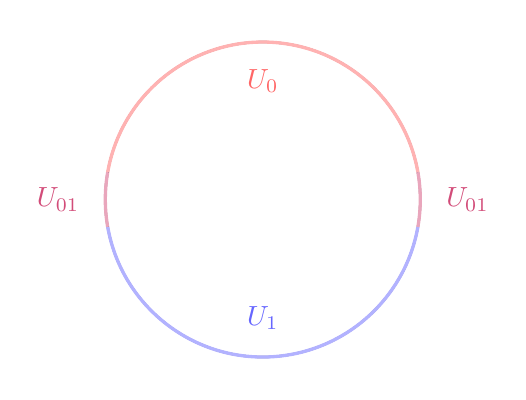
\begin{tikzpicture}[scale=2]
  % circle
  \draw[thick] (0,0) circle (1);

  % upper and lower "open" sets as thick arcs (leaving small gaps at left/right)
  \draw[very thick, blue!30]
    (-170:1) arc[start angle=-170, end angle=-10, radius=1];
  \draw[very thick, red!30]
    (170:1) arc[start angle=170, end angle=10, radius=1];

  % optional: lightly indicate the overlap neighborhoods near left/right
  \draw[very thick, purple!35]
    (-10:1) arc[start angle=-10, end angle=10, radius=1];
  \draw[very thick, purple!35]
    (170:1) arc[start angle=170, end angle=190, radius=1];

  % labels for the open sets
  \node[red!60] at (0,0.75) {$U_0$};
  \node[blue!60]  at (0,-0.75) {$U_1$};

  % labels for overlaps (optional)
  \node[purple!70] at (1.3,0) {$U_{01}$};
  \node[purple!70] at (-1.3,0) {$U_{01}$};

\end{tikzpicture}
\end{figure}

Note that $\check{C}^1(\mathcal{U},F) = \Z^{\times 2}$ in this instance, since $U_0 \cap U_1$ has two connected components. The chain complex here then looks like
\begin{align*}
    \check{C}^\bullet(\mathcal{U},F) : \quad\quad 0 \to \Z \oplus \Z \xto{\begin{pmatrix} 1 & -1 \\ 1 & -1\end{pmatrix}} \Z \oplus \Z \to 0 \to \cdots
\end{align*}
so we get cohomology in degrees $0$ and $1$, as expected. This is an example of how \emph{refining} the cover can detect more cohomological features.
\end{example}

\begin{proposition}\label{prop:Cech-0-is-global-sections} 
For any space $X$ and any \emph{sheaf} $F\in\Ab(X)$, we have a canonical isomorphism
\begin{align*}
    \check{H}^0(X,F) \cong \Gamma(X,F).
\end{align*}
\end{proposition}
\begin{proof} Given any open cover $\mathcal{U} = \left\{ U_i \right\}$, an element $f \in \check{H}^0(\mathcal{U},F)$ is an element $f_i \in F(U_i)$ for each $i$ (this is the condition of lying in $C^0(\mathcal{U},F)$), which lies in the kernel of $\delta^0 \colon C^0 \to C^1$. This means that $f_{i|U_i\cap U_j} = f_{j|U_i\cap U_j}$ for each $i,j$. Since $F$ is a sheaf, by gluing, the $f_i$'s glue together to give a well-defined global section $f\in \Gamma(X,F)$. This is easily seen to be an isomorphism.
\end{proof}

\begin{exercise} Verify that \v{C}ech cohomology is functorial in the sheaf, that is for any $X$ and any $q\ge 0$ we have a functor
\begin{align*}
    \check{H}^q(X,-) \colon \Ab(X) \to \Ab.
\end{align*}
\end{exercise}

Before we get to \Cref{prop:LES-Cech-cohomology-presheaves} it's worth saying some words about exactness of sheaves versus presheaves.

\begin{remark}[On exactness] By definition, a sequence of presheaves $F_1\to F_2 \to F_3$ on $X$ is exact if
\begin{align*}
    0 \to F_1(U) \to F_2(U) \to F_3(U) \to 0
\end{align*}
is an exact sequence of abelian groups for all $U \in \Open(X)$. If these are all sheaves, then we say the sequence is exact if
\begin{align*}
    0 \to (F_1)_x \to (F_2)_x \to (F_3)_x \to 0
\end{align*}
is exact for every point $x\in X$. If a sequence of sheaves is exact (when considered as presheaves) then it is still exact when considered as sheaves, e.g. by \Cref{cor:filtered-colimits-preserve-exactness} or by the phrase ``sheafification is exact.'' The converse \emph{does not hold}! Consider the short exact sequence of sheaves
\begin{align*}
    0 \to \underline{\Z} \to C^0(-,\R) \to C^0(-,S^1) \to 0.
\end{align*}
This is exact (over any space $X$) since it is exact in each fiber. However over an arbitrary space it won't be exact as a sequence of presheaves, because not every circle-valued function lifts to a real-valued function (e.g. if it has non-trivial winding number).\footnote{Indeed we can think of the winding number as measuring the failure of lifting, giving us a class in $H^1(X,\underline{\Z}) = [X,S^1]$.}
\end{remark}

\begin{exercise}\label{exer:mono-sheaves-is-mono-presheaves} If $F \to G$ is a map of presheaves which is a monomorphism of sheaves (it is injective on every stalk) then it is a monomorphism of presheaves (it is injective on every section).
\end{exercise}


\begin{proposition}\label{prop:LES-Cech-cohomology-presheaves} 
If
\begin{align*}
    0 \to F_1 \to F_2 \to F_3 \to 0
\end{align*}
is a short exact sequence \emph{of presheaves}, it induces a long exact sequence
\begin{align*}
    0 &\to \check{H}^0(X,F_1) \to \check{H}^0(X,F_2) \to \check{H}^0(X,F_3) \\
    &\to \check{H}^1(X,F_1) \to \check{H}^1(X,F_2) \to \check{H}^1(X,F_3) \\
    &\to \check{H}^2(X,F_1) \to \cdots
\end{align*}
\end{proposition}
\begin{proof}[Sketch] The first step is to show that, for any cover $\mathcal{U}$, the functor
\begin{align*}
    \check{C}^q(\mathcal{U},-) \colon \Fun(\Open(X)^\op,\Ab) \to \Ab
\end{align*}
is exact (subtlety: its restriction to $\Ab(X)$ is not necessarily exact, because $\Ab(X)$ has a different notion of exactness than the presheaf category!). A diagram chase then implies we get a long exact sequence on $\check{H}^\ast(\mathcal{U},-)$. Then we take a colimit over all $\mathcal{U}$ in the filtered category of covers $\Cov(X)$, and use that filtered colimits preserve exactness to conclude (\Cref{exa:CovX-filtered} and \Cref{cor:filtered-colimits-preserve-exactness}). The details are spelled out in \cite[pp.~28--29]{Hirzebruch}.
\end{proof}

This begs a very interesting question --- when do the \v{C}ech cohomology of a presheaf $F$ and of its sheafification $F^\sharp$ agree? We need two preliminary results to lead up to a partial answer to this question.

\begin{proposition}\label{prop:property-of-pshf-sheafifying-to-zero} 
Let $F$ be a presheaf over a space, and suppose $F^\sharp = 0$. For any point $x\in X$, any open $U\ni x$ and any $f\in F(U)$, there exists some smaller open neighborhood $V \subseteq U$ containing $x$ for which $f_{|V} = 0$. 
\end{proposition}
\begin{proof} This is because the stalk $F_x = F^\sharp_x$ must be zero.
\end{proof}



\begin{lemma}\label{lem:presheaf-sheafifying-to-zero-has-no-cohomology} 
Let $X$ be a paracompact space, and $F$ a presheaf on $X$. Then if $F^\sharp$ is the zero sheaf, we claim that $\check{H}^n(X,F) = 0$ for all $n\ge0$.
\end{lemma}
\begin{proof} We show that no cochains survive refinement. That is, if $f \in \check{C}^q(\mathcal{U},F)$ for some cover $\mathcal{U} = \{U_i\}_{i\in I}$, we will find a refinement of the cover which kills $f$. Without loss of generality assume that $\mathcal{U}$ is locally finite. By the Dieudonn\'e shrinking theorem (\Cref{thm:shrinking}), we may find a cover $\mathcal{W} = \left\{ W_i \right\}_{i\in I}$ for which $\overline{W_i} \subseteq U_i$.

Let $J = X$ as a set--- we will produce a refinement of the cover $\mathcal{U}$, now indexed over $J$. For each $x\in X$, we pick an open neighborhood $V_x \ni x$ for which:
\begin{enumerate}
    \item if $x\in U_i$ then $V_x \subseteq U_i$ and if $x\in W_i$ then $V_x \subseteq W_i$
    \item if $V_x \cap W_i \ne \emptyset$ then $V_x \subseteq U_i$
    \item if $x\in U_{i_0} \cap \cdots \cap U_{i_q}$ then $f(i_0, \ldots, i_q)$ restricts to zero in $F(V_x)$.
\end{enumerate}
Since $\mathcal{U}$ and $\mathcal{W}$ are locally finite, there are only finitely many $U_i$ and $W_i$ containing $x$ to worry about, so the first two conditions can be fulfilled. Why are we allowed to guarantee the last condition can hold? By \Cref{prop:property-of-pshf-sheafifying-to-zero} some sufficiently small neighborhood of $x$ in $U_{i_0} \cap \cdots \cap U_{i_q}$ will have the property that $f(i_0, \ldots, i_q)$ restricts to zero in it. We can pick $V_x$ to be that neighborhood, perhaps intersecting it further finitely many times to make it satisfy the first two conditions.

We now claim that $f$ refines to zero in this new cover $\left\{ V_x \right\}_{x\in X}$. Pick any tuple $(x_0, \ldots, x_q)$, and let $i_j$ be such that $x_j \in W_{i_j} \subseteq U_{i_j}$ for each $j$. By (1), this tells us that $V_{x_j} \subseteq W_{i_j} \subseteq U_{i_j}$. We want to argue that the image of $f(i_0, \ldots, i_p)$ under the restriction map
\begin{align*}
    F(U_{i_0} \cap \cdots \cap U_{i_q}) \to F(V_{x_0}\cap \cdots \cap V_{x_q})
\end{align*}
is zero. If the intersection of the $V_{x_i}$'s is empty, there is nothing to show, so suppose it is nonempty. Then $V_{x_0}\cap V_{x_k}$ is nonempty for each $k$. Since $V_{x_k} \subseteq W_{i_k}$, we have that $V_{x_0} \cap W_{i_k} \ne \emptyset$, and by point (2) this implies that $V_{x_0} \subseteq U_{i_k}$. Since this is true for all $k$, we have that $V_{x_0} \subseteq U_{i_0} \cap \cdots \cap U_{i_q}$. However by (3), since $x_0 \in V_{x_0}\subseteq U_{i_0} \cap \cdots \cap U_{i_q}$, we have that $f(i_0, \ldots, i_q)$ restricts to zero on $V_{x_0}$ and therefore on the smaller subset $V_{x_0} \cap \cdots \cap V_{x_q}$.
\end{proof}


\begin{theorem}\label{thm:paracompact-space-Cech-cohomology-of-sheafification} 
If $X$ is paracompact, and $F$ is a presheaf with corresponding sheaf $F^\sharp$, then the natural map $\check{H}^q(X,F) \to \check{H}^q(X,F^\sharp)$ is an isomorphism for all $q\ge0$.
\end{theorem}
\begin{proof} Consider the sheafification map $F \to F^\sharp$ and take its kernel and cokernel in the category of presheaves
\begin{align*}
    0 \to K \to F \to F^\sharp \to C \to 0.
\end{align*}
As $F \to F^\sharp$ sheafifies to an isomorphism, and since sheafification is an exact functor, we have that $K$ and $C$ sheafify to zero. Hence their higher cohomology vanishes by \Cref{lem:presheaf-sheafifying-to-zero-has-no-cohomology}, and using the long exact sequence on cohomology attached to short exact sequences of presheaves, we obtain that the induced maps $\check{H}^q(X,F) \to \check{H}^q(X,F^\sharp)$ are all isomorphisms.
\end{proof}

So over paracompact spaces, there is no difference between the cohomology of a presheaf and of its resulting sheafification. A corollary of this we will use often is the following:

\begin{proposition}\label{prop:LES-Cech-cohomology}
If $X$ is a paracompact space, and $0 \to F_1 \to F_2 \to F_3 \to 0$ is an exact sequence of \emph{sheaves} on $X$, then it induces a long exact sequence
\begin{align*}
    0 \to \check{H}^0(X,F_1) \to \check{H}^0(X,F_2) \to \check{H}^0(X,F_3) \to \check{H}^1(X,F_1) \to \cdots
\end{align*}
\end{proposition}
\begin{proof} Let $F_1 \to F_2 \to F_3$ be a short exact sequence of \emph{sheaves}. Define a \emph{presheaf} $F_2/F_1$ to be the cokernel of the map $F_1 \to F_2$ in the category of sheaves. By \Cref{prop:LES-Cech-cohomology-presheaves} we get a long exact sequence on \v{C}ech cohomology of presheaves
\begin{align*}
    0 \to \check{H}^0(X,F_1) \to \check{H}^0(X,F_2) \to \check{H}^0(X, F_2/F_1) \to \check{H}^1(X,F_1) \to \cdots 
\end{align*}
Note that $F_1$ and $F_2$ are already sheaves, and we claim that the natural map $(F_2/F_1)^\sharp \to F_3$ is an isomorphism. This is clear since sheafification is exact. Therefore by \Cref{thm:paracompact-space-Cech-cohomology-of-sheafification} we have canonical isomorphisms $\check{H}^q(X,F_2/F_1) \xto{\sim} \check{H}^q(X,F_3)$ for any $q\ge0$. Plugging these into the sequence above we get our desired result.
\end{proof}

\subsection{Acyclic resolutions}

In classical topology, spaces were called \emph{acyclic} if every cycle on the space was a boundary --- in other words the space had the homology type of a point or any contractible space. Similarly a connective cochain complex can be considered acyclic if its cohomology is concentrated in degree zero. For \v{C}ech cohomology, we say a sheaf is acyclic if its \v{C}ech cochains complex is an acyclic complex. In other words:

\begin{definition}\label{def:acyclic-sheaf} A sheaf $F\in \Ab(X)$ is \emph{acyclic} if $\check{H}^p(X,F) = 0$ for $p>0$.
\end{definition}

\begin{definition} Take $F\in \Ab(X)$. An \emph{acyclic resolution} of $F$ is a (possibly infinite) exact sequence
\begin{align*}
    0 \to F \to A^0 \to A^1 \to \cdots
\end{align*}
where each $A^i$ is acyclic for $i\ge 0$.
\end{definition}

\begin{exercise}\label{exer:global-sections-left-exact} 
Argue that the global sections functor
\begin{align*}
    \Gamma(X,-) \colon \Ab(X) \to \Ab
\end{align*}
is left exact, and then argue that it sends an acyclic resolution of $F$ to a chain complex in $\Ab$.
\end{exercise}

It turns out we can use acyclic resolutions to compute cohomology!

\begin{theorem}[\v{C}ech=sheaf cohomology] 
\label{thm:cech-equals-sheaf}
Let $F\in \Ab(X)$ be a sheaf over a paracompact space, and consider any acyclic resolution $F \to A^\bullet$. Then $\check{H}^q(X,F)$ is canonically isomorphic to the cohomology of the chain complex obtained by applying $\Gamma(X,-)$ to the acyclic resolution.
%, which by taking the acyclic sheaves to actually be injective is isomorphic to $H^q^\asst(X,F)$.
\end{theorem}
\begin{proof} We write out the sequence we're looking at:
\begin{align*}
    \Gamma(X,A^0) \xto{d^0} \Gamma(X,A^1) \xto{d^1} \cdots
\end{align*}
We will proceed by induction on $q$. 

\emph{Base case $q=0$}: Since $\Gamma(X,-F)$ is a left exact functor (\Cref{exer:global-sections-left-exact}), we get that
\begin{align*}
    0 \to \Gamma(X,F) \to \Gamma(X,A^0) \xto{d^0_\ast} \Gamma(X,A^1)
\end{align*}
is left exact. In particular, we get that the kernel of $d^0_\ast$ is exactly $\Gamma(X,F)$, which agrees with $\check{H}^0(X,F)$ by \Cref{prop:Cech-0-is-global-sections}. Hence $\check{H}^0(X,F)$ is the $0$th cohomology of $\Gamma(X,-)$ applied to the acyclic resolution, establishing our base case.

\emph{Inductive step}: For any $p\ge0$, we let $K^p := \ker(A^p \to A^{p+1})$. Note by definition of our resolution, we have that $K^0\cong F$. By exactness and the first isomorphism theorem, $A^p/K^p \cong K^{p+1}$, so we get short exact sequences of sheaves for each $p\ge 0$:
\begin{align*}
    0 \to K^p \to A^p \to K^{p+1}\to 0.
\end{align*}
Applying the long exact sequence on cohomology (\Cref{prop:LES-Cech-cohomology}), we get
\begin{align*}
    \cdots \to \check{H}^q(X,K^p) \to \check{H}^q(X,A^p) \to \check{H}^q(X,K^{p+1})\xto{\partial} \check{H}^{q+1}(X,K^p) \to \check{H}^{q+1}(X,K^p) \to \cdots
\end{align*}
Since the $A^p$'s are acyclic, the boundary maps $\partial$ are isomorphisms $\check{H}^q(X,K^{p+1})\cong \check{H}^{q+1}(X,K^p)$ for $q\ge 1$. Note though that $K^0 = F$, so we get that
\begin{align*}
    \check{H}^1(X,K^{q-1}) \cong \check{H}^q(X,F) \quad\quad \text{for }q\ge1.
\end{align*}
We claim $\check{H}^1(K^{q-1})$ is identified canonically with the $q$th cohomology of the sequence $\left\{ \Gamma(X,A^i) \right\}$. Indeed this follows from looking at the long exact sequence attached to $0 \to K^{q-1} \to A^{q-1}\to K^q \to 0$, from which we get
\begin{align*}
    H^0(X,A^{q-1}) \xto{d^{q-1}_\ast} H^0(X,K^q) \to H^1(X,K^{q-1}) \to 0.
\end{align*}
Since $H^0(X,K^q) = \ker(d^q_\ast)$, we have that $H^1(X,K^{q-1})$ is $\ker(d^q_\ast)$ modulo the image of $d^{q-1}_\ast$, hence it is the cohomology of the complex.
\end{proof}

This provides us a new way to compute \v{C}ech cohomology over a paracompact space!

\begin{definition} Recall an \textit{injective sheaf} is an injective object in $\Ab(X)$, meaning that the functor
\begin{align*}
    \Hom_{\Ab(X)}(-,I) \colon \Ab(X)^\op \to \Ab
\end{align*}
is exact.
\end{definition}

\begin{example}\label{exa:skyscraper-injective} 
Let $I$ be an injective abelian group, and $i \colon \{x\} \to X$ the inclusion of a point. Then the skyscraper sheaf $i_\ast I \in \Ab(X)$ is injective.
\end{example}
\begin{proof} The data of a map into a skyscraper sheaf is completely determined by what happens on the stalk over $x$ (this is a pullback-pushforward adjunction) -- this gives us a natural isomorphism of functors $\Ab(X) \to \Ab$:
\begin{align*}
    \Hom_{\Ab(X)}(-, i_\ast I) \cong \Hom_{\Ab}((-)_x, I).
\end{align*}
the right hand side is exact since taking stalks is an exact functor, hence $i_\ast I$ is injective.
\end{proof}

\begin{definition}\label{def:injective-resolution} Let $F\in \Ab(X)$ be a sheaf. An \emph{injective resolution} of $F$ is an exact sequence
\begin{align*}
    0 \to F \to I^0 \to I^1 \to I^2 \to \cdots
\end{align*}
for which each sheaf $I^j$ is injective.
\end{definition}

\begin{remark} In general, one deals with \emph{injective resolutions} rather than acyclic ones. This allows us to reword the above in the language of derived categories, and define cohomology as the right derived functors of the global sections functor. In order to do this, we should show that injective sheaves are in fact acyclic.
\end{remark}

First we need a lemma.
\begin{lemma}[{\cite[03AS, 03AU]{Stacks}}] Let $X$ be any space, and $\mathcal{U} = \left\{ U_i \right\}$ any open cover. Define a chain complex of abelian sheaves $\Z_{\mathcal{U},\bullet}$ by
\begin{align*}
    \Z_{\mathcal{U},p} = \bigoplus_{i_0, \ldots, i_p} \Z_{U_{i_0}\cap \cdots \cap U_{i_p}},
\end{align*}
where recall $\Z_U$ is the sheaf corepresenting $\Gamma(U,-)$ as in \Cref{exa:ZU-sheaf}. The differentials on the chain complex $\Z_{\mathcal{U},\bullet}$ are the sum over $(-1)^k$ times the canonical map
\begin{align*}
    \Z_{U_{i_0}\cap \cdots \cap U_{i_p}} \to \Z_{U_{i_0}\cap \cdots\cap \widehat{U_{i_k}} \cap U_{i_p}}.
\end{align*}
Then we claim that $\Hom_{\Ab(X)} \left( \Z_{\mathcal{U},p},F \right)\cong \check{C}^p(\mathcal{U},F)$ for any $F\in \Ab(X)$, and that the differentials $\Z_{\mathcal{U},p+1} \to \Z_{\mathcal{U},p}$ induce the \v{C}ech cochain differentials $\delta^p \colon \check{C}(\mathcal{U},F) \to \check{C}^{p+1}(\mathcal{U},F)$ after applying $\Hom_{\Ab(X)}(-,F)$.
\end{lemma}

\begin{corollary}\label{cor:injective-sheaf-is-acyclic} 
Every injective sheaf is acyclic.
\end{corollary}
\begin{proof} If $I \in \Ab(X)$ is injective, then $\Hom_{\Ab(X)}(-,I)$ is an exact functor. In particular it sends $\Z_{\mathcal{U},\bullet}$ to a cochain complex which is exact except for in the first term. Since this is exactly the \v{C}ech cochains complex, this implies that $\check{H}^q(\mathcal{U},I) = 0$ for $q\ge 1$. As this is true for every $\mathcal{U}$, we conclude that $\check{H}^q(X,I) = 0$ for all $q\ge 1$.
\end{proof}

The converse does not hold:

\begin{example} Let $A$ be a non-injective abelian group, and $i \colon \{x\} \to X$ the inclusion of a point. Then we claim the skyscraper sheaf $i_\ast A$ is acyclic but need not be injective.
\end{example}
\begin{proof} Take any cover of $X$ and refine it so that $U_0\ni x$ and $U_i\not\ni x$ for $i>0$. In particular there are no sections of $i_\ast A$ over overlaps, so $\check{H}^q(\mathcal{U},i_\ast A) = 0$ for all $q>0$. This remains true under refinement, so this vanishing passes to the colimit. Failure of injectivity of the sheaf $i_\ast A$ reduces to failure of injectivity of $A$ as an abelian group by looking at maps on stalks as in the proof of \Cref{exa:skyscraper-injective}.
\end{proof}


So \Cref{cor:injective-sheaf-is-acyclic} lets us conclude what we may have already expected:

\begin{corollary}\label{cor:cech-equals-sheaf-cohomology-paracompact-Hausdorff} 
Over a paracompact Hausdorff space $X$, we have that \v{C}ech cohomology is canonically isomorphic to the right derived functors of global sections.
\end{corollary}

\begin{remark} The contemporary perspective is to \emph{first} define cohomology as these right derived functors, \emph{then} to compare with \v{C}ech cohomology. The classical perspective of Serre, Godement and others, and what we presented above, is the exact opposite.
\end{remark}

\begin{exercise} Note that \Cref{thm:cech-equals-sheaf} has already told us that cohomology can be computed using an injective resolution, and that this doesn't depend on the choice of injective resolution. The yoga of derived functors lets us conclude this also. If we wanted to try to prove it by hand, we could do it as follows: Prove that if $F \to I^\bullet$ is any injective resolution and $F \to J^\bullet$ is any other resolution, there exists a map of chain complexes $f^\bullet$ making the diagram commute:
\[ \begin{tikzcd}
    F\rar\ar[dr] & I^\bullet\dar["f^\bullet" right]\\
     & J^\bullet.
\end{tikzcd}\]
Show that $f^\bullet$ is a quasi-isomorphism and moreover is well-defined up to chain homotopy.
\end{exercise}

\subsection{Existence of injectives}

We now know a new way to take cohomology, which is leveraging an acyclic resolution, or if we want to use some category theory, take the derived functors of global sections. This perspective is only valuable if we can actually find acyclic/injective resolutions. How do we know they even exist? Let's argue that they do.

\begin{proposition}\label{prop:abX-enough-injectives} 
For every $F \in \Ab(X)$, there exists an injective sheaf $I$ and a monomorphism $F \to I$.
\end{proposition}
\begin{proof} We can embed the abelian group $F_x$ into an injective abelian group $I_x$. Define a presheaf by
\begin{align*}
    \mathcal{I} \colon \Open(X)^\op &\to \Ab \\
    U &\mapsto \prod_{x\in U}I_x.
\end{align*}
Note that $\mathcal{I}$ is actually a sheaf, since it is a product of skyscraper sheaves, one for each point of $X$. Observe that the stalk of the sheaf $\mathcal{I}_x$ need not be equal to $I_x$, however it will contain $I_x$ as a retract. We claim that
\begin{align*}
    \Hom_{\Ab(X)}(F,\mathcal{I}) \cong \prod_{x\in X}\Hom_\Ab(F_x,I_x).
\end{align*}
There is a map from the left to the right by taking $g \colon \mathcal{F}(U) \to \mathcal{I}(U)$ for any open $U\ni x$, then noting that $\mathcal{F}(U) \to \mathcal{I}(U)$ maps to $I_x$ along the projection, then taking a colimit over $U$, inducing $\mathcal{F}_x \to \mathcal{I}_x$. For the reverse direction, if we have maps $f_x \colon F_x \to I_x$ for each $x$, we can define $F(U) \to \mathcal{I}(U)$ by the composite
\begin{align*}
    F(U) \to \prod_{x\in U} F_x \xto{\prod f_x} \prod_{x\in U} I_x = \mathcal{I}(U),
\end{align*}
and we have these maps on each section, which give a map of sheaves. We claim these are inverse operations.

We have to check two things: that $\mathcal{I}$ is injective, and that $F \to \mathcal{I}$ is a monomorphism. That it is a monomorphism can be seen sectionwise, which induces monomorphisms on stalks since filtered colimits preserve monomorphisms.

To see $\mathcal{I}$ is injective, it suffices to show observe each skyscraper sheaf is injective by \Cref{exa:skyscraper-injective} and then use that injective objects are closed under arbitrary products.
\end{proof}

\begin{corollary} For any space $X$, we have that every $F\in\Ab(X)$ admits an injective resolution.
\end{corollary}
\begin{proof} By \Cref{prop:abX-enough-injectives}, we start with
\begin{align*}
    0 \to F \to I^0,
\end{align*}
and then take the quotient $I^0/F$ and embed it in some injective $I^1$. The composite $F \to I^0 \to I^1$ is obviously zero since it factors through the quotient by construction, so we get
\begin{align*}
    0 \to F \to I^0 \to I^1.
\end{align*}
We then embed $I^1/I^0$ into some injective $I^2$, and so on.
\end{proof}

\subsection{Godement resolutions}

We can expand the results of the previous section by establishing the so-called \emph{Godement resolution}, which is a functorial way of producing an acyclic resolution. We first need some preliminary definitions:

\begin{definition}\label{def:pullback-pushforward} Let $f \colon X \to Y$ be a continuous map of spaces.
\begin{itemize}
    \item Given a sheaf $F\in \Ab(X)$, we define the \emph{pushforward sheaf} $f_\ast F$ on $Y$ by the rule
    \begin{align*}
        f_\ast F \colon \Open(Y) &\to \Ab \\
        U &\mapsto F(f^{-1}(U)).
    \end{align*}
    We claim that $f_\ast F$ satisfies locality and gluing (exercise) and therefore $f_\ast$ induces a functor which we call \emph{pushforward}:
    \begin{align*}
        f_\ast \colon \Ab(X) \to \Ab(Y)
    \end{align*}
    %
    \item Given a sheaf $G\in \Ab(Y)$, we define a presheaf on $X$ by
    \begin{align*}
        f^{-1}_\text{pre}G \colon \Open(X) &\to \Ab \\
        U &\mapsto \colim_{\substack{V\in \Open(Y) \\ V \supseteq f(U)}} G(V).
    \end{align*}
    We define the \emph{inverse image sheaf} to be the sheafification of this, that is $f^{-1}G := (f^{-1}_\text{pre}G)^\sharp$. Again we claim this is functorial:
    \begin{align*}
        f^{-1} \colon \Ab(Y) \to \Ab(X).
    \end{align*}
\end{itemize}
\end{definition}

\begin{example} In the particular case when our map is of the form $i \colon \left\{ x \right\} \to X$, that is, the inclusion of a point, we have that a sheaf on the one-point space is just a single abelian group $A$. The pushforward sheaf $i_\ast A$ is \emph{exactly} the skyscraper sheaf of $A$ at the point $x \in X$. This is the reason for the notation for skyscraper sheaves in \Cref{exa:skyscraper-sheaves}.
\end{example}

\begin{proposition}\label{prop:pullback-pushforward-adjunction} Let $f \colon X \to Y$ be any map of spaces. Then pullback and pushforward form an adjunction:
\begin{align*}
    f^{-1} \colon \Ab(Y) \leftrightarrows \Ab(X) \colon f_\ast.
\end{align*}
\end{proposition}
\begin{proof} For a proof (in slightly more generality), see the arguments in \cite[008P]{Stacks} and the previous sections.
\end{proof}

\begin{remark} Right adjoints preserve injective objects, so the pushforward of an injective sheaf is still injective. In particular pushforward of an injective abelian group (viewed as an injective sheaf over a point) is still injective. This is alternative way to see that skyscraper sheaves of injective abelian groups are injective sheaves (\Cref{exa:skyscraper-injective}). And indeed, we essentially used the adjunction \Cref{prop:pullback-pushforward-adjunction} to prove it.
\end{remark}

An interesting case comes from \emph{forgetting} the topology on $X$, and considering pullback-pushforward along the resulting natural map.

\begin{notation} For any space $X$, we denote by $X^\delta$ the topological space with the exact same underlying set as $X$, but with the discrete topology (every subset is open). There is a natural map $\epsilon \colon X^\delta \to X$.\footnote{There is a ``discrete-forgetful'' adjunction $(-)^\delta \colon \Set \leftrightarrows \Top \colon U$, where $U$ forgets the topology on a space and returns its underlying set, and $(-)^\delta$ endows a set with the discrete topology. This map $X^\delta \xto{\epsilon} X$ is simply the counit of this adjunction, hence is natural in $X$.}
\end{notation}

We define a functor
\begin{align*}
    C^0 \colon \Ab(X) &\to \Ab(X) \\
    F &\mapsto \epsilon_\ast \epsilon^{-1} F.
\end{align*}
%
As a presheaf, $\epsilon_\ast \epsilon^{-1} F$ sends $U$ to $\prod_{x\in U} F_x$, that is, it is the sheaf of germs at all points. It is also clear that it comes equipped with a natural map of sheaves $j \colon F \to C^0(F)$ (which is the unit of the pullback-pushforward adjunction).

\begin{proposition}\label{prop:godement-sheaves-are-acyclic} 
Let $X$ be an arbitrary space, and $F\in \Ab(X)$ any sheaf of abelian groups.
\begin{enumerate}
    \item The map $j \colon F \to C^0(F)$ is a monomorphism.
    \item The sheaf $C^0(F)$ is acyclic
\end{enumerate}
\end{proposition}
\begin{proof} The first point is immediate -- if $f,g\in F(U)$ have the property that $j(f) = j(g) \in C^0(F)(U) = \prod_{x\in U}F_x$, this means they have the same value on stalks of all points in $U$, which by the sheaf condition means they must agree. The difficult part is the second point, arguing that $C^0(F)$ is acyclic.

Fix any open cover $\mathcal{U} = \left\{ U_i \right\}_{i\in I}$ of $X$. We have that the \v{C}ech $p$-cochains of $C^0(F)$ can be rewritten (by swapping products around) as:
\begin{align*}
    \check{C}^p(\mathcal{U},C^0(F)) &= \prod_{i_0, \ldots, i_p\in I} C^0(F)(U_{i_0} \cap \cdots \cap U_{i_p}) = \prod_{i_0, \ldots, i_p\in I}\prod_{x\in U_{i_0}\cap \cdots \cap U_{i_p}}F_x \\
    &= \prod_{x\in X} \prod_{\substack{i_0, \ldots, i_p\in I \\ U_{i_0}\cap \cdots \cap U_{i_p}\ni x}}F_x.
\end{align*}
So the \v{C}ech differential acts pointwise on each $x$. In other words if we define
\begin{align*}
    \check{C}^p(\mathcal{U},x,F) := \prod_{\substack{i_0, \ldots, i_p\in I \\ U_{i_0}\cap \cdots \cap U_{i_p}\ni x}}F_x,
\end{align*}
then it is clear that $\check{C}^\bullet(\mathcal{U},C^0(F))$ is a product over the individual complexes $\check{C}^\bullet(\mathcal{U},x,F)$. It therefore reduces to showing that $\check{C}^\bullet(\mathcal{U},x,F)$ is an acyclic complex.

Fix an arbitrary point $x\in X$, and find one index $i'\in I$ for which $x\in U_{i'}$. Then (if we use \emph{unnormalized \v{C}ech cochains}\footnote{There are two notions of \v{C}ech cochains, one is \emph{normalized}, where each of $i_0, \ldots, i_p$ needs to be distinct, and the other is \emph{unnormalized}, where we're allowed to have repetitions. They end up giving completely the same answer, but some operations like this one are much easier to state in the language of unnormalized cochains.}) we can define a chain homotopy
\begin{align*}
    h \colon \check{C}^p(\mathcal{U},x,F) &\to \check{C}^{p-1}(\mathcal{U},x,F),
\end{align*}
by defining $(hc)(i_0, \ldots, i_{p-1}) = c(i',i_0, \ldots, i_{p-1})$. We can check, for $p\ge1$, this is a null-homotopy for the identity map on the cochain complex. Therefore $\check{C}^p(\mathcal{U},x,F)$ has no cohomology above $H^0$, and therefore neither does $\check{C}^p(\mathcal{U},C^0(F))$.
\end{proof}

Since $C^0$ is functorial, we can use it to (functorially!) build an acyclic resolution.

\begin{notation} We define $C^1 \colon \Ab(X) \to \Ab(X)$ to be the functor sending $F$ to $C^0(\coker(F \xto{j}C^0(F)))$, that is, we look at $j \colon F \to C^0(F)$, take its cokernel, and then hit it with $C^0$. We get a composite map which we call $d^0$:
\begin{align*}
    C^0(F) \to \coker(j) \to C^0(\coker(j)) =: C^1(F),
\end{align*}
and it is clear that the composite $F \to C^0(F) \to C^1(F)$ is zero, since it factors through the cokernel of $F$.

Iteratively, we define
\begin{align*}
    C^{n+1}(F) = C^0(\coker(C^{n-1}(F) \xto{d^{n+1}} C^n(F)),
\end{align*}
which receives an analogous map $d^n$ from $C^n(F)$.
\end{notation}

\begin{definition}\label{def:godement-resolution} 
We define the \textit{Godement resolution} to be the acyclic resolution of $F$ obtained as
\begin{align*}
    0 \to F \to C^0(F) \xto{d^0} C^1(F) \xto{d^1} C^2(F) \to \cdots 
\end{align*}
as above.
\end{definition}

\begin{remark} A few things about this are worth noting:
\begin{itemize}
    \item each of these constructions $C^n$ are \emph{functorial}
    \item the functors $C^n(-) \colon \Ab(X) \to \Ab(X)$ are exact for each $n$.
\end{itemize}
Exactness of $C^0(-)$ is immediate, since it is a stalkwise construction, and exactness of $C^n(-)$ can be proved inductively.
\end{remark}

What is the benefit of all this nonsense? It allows us to give an analogue and a reproof of \Cref{prop:LES-Cech-cohomology} (on a paracompact space, a short exact sequences of sheaves induces a long exact sequence on cohomology) for sheaf cohomology, and \emph{without paracompactness}.

\begin{proposition}\label{prop:LES-sheaf-cohomology-any-space} Let $X$ be any topological space, and let $0 \to F_1 \to F_2 \to F_3 \to 0$ be a short exact sequence of sheaves on $X$. This induces a long exact sequence on sheaf cohomology
\begin{align*}
    0 \to H^0(X,F_1) \to H^0(X,F_2) \to H^0(X,F_3) \to H^1(X,F_1) \to \cdots
\end{align*}
\end{proposition}
\begin{proof} We build the Godement resolutions $F_i \to C^\bullet(X,F_i)$ functorially for each $i=1,2,3$, and exactness of the $C^n$ functors implies that $C^\bullet(X,F_1) \to C^\bullet(X,F_2) \to C^\bullet(X,F_3)$ is a short exact sequence \emph{of chain complexes}. A standard diagram chase argument gives the desired long exact sequence on cohomology.
\end{proof}

When $X$ is paracompact, sheaf cohomology agrees with \v{C}ech cohomology, so the previous result lets us reprove \Cref{prop:LES-Cech-cohomology}.

\begin{remark} While $C^n(F)$ is acyclic, there is no reason to expect it to be injective. A modified construction works, however, to produce functorial injective resolutions:
\begin{enumerate}
    \item begin with a functorial injective embedding of abelian groups into injective ones
    \item modify the construction of $C^0(F)$ by applying this functor to each stalk
    \item take the inclusion, cokernel, iterate.
\end{enumerate}
Details are in \cite[01DG]{Stacks}.
\end{remark}


\subsection{Fine sheaves}

Another source of acyclic sheaves comes from so-called \emph{fine sheaves} on paracompact spaces.

\begin{definition}\label{def:fine-sheaf} 
Let $F$ be a sheaf over a paracompact space $X$. We say that $F$ is \emph{fine} if, for every locally finite open covering $\left\{ U_i \right\}$ of $X$, we have a system of homomorphisms
\begin{align*}
    h_i \colon F \to F,
\end{align*}
so that
\begin{enumerate}
    \item For every $i$, the support of $h_i$ is closed in $X$ and contained in $U_i$
    \item $\sum_i h_i$ is the identity (the sum makes sense because the cover is locally finite).
\end{enumerate}
\end{definition}


% \todo{in Bredon II.9.15, he says $A$ is fine if $\Hom(A,A)$ is soft. is this a good characterization for us to use?}


\begin{example}\label{exa:cx-valued-cts-funcs-is-fine} 
The sheaf $C^0(-,\C)$ of germs of complex-valued continuous functions over a paracompact space is fine.
\end{example}
\begin{proof} Fix a locally finite open cover $\left\{ U_i \right\}$, and pick a partition of unity $\{\phi_i\}$. Then we can define
\begin{align*}
    h_i \colon C^0(-,\C) &\to C^0(-,\C) \\
    f &\mapsto f\cdot \phi_i.
\end{align*}
It is clear the $h_i$'s sum to the identity, and the closed subsets in the definition of fineness are given by their support.
\end{proof}

\begin{example} If $X$ is a differentiable manifold, then the sheaf of germs of differentiable functions $\mathbb{C}_{\mathfrak{b}}$ is fine.
\end{example}
\begin{proof} The same proof works, aside from one subtlety -- in order for $h$ to be a map of sheaves, we can't just multiply by arbitrary $\phi_i$, since this might break differentiability--- we need the $\phi_i$'s themselves to be differentiable. Hence this hinges on the existence of a differentiable partition of unity, which was proven by de Rham (at least in the smooth setting? see \cite[I.2]{derhamDifferentiableManifolds1984}). 
\end{proof}

\begin{remark} If $X$ is a complex manifold and $\mathcal{O}_X$ is the sheaf of holomorphic functions, it is not necessarily the case that $\mathcal{O}_X$ is fine. An analogous argument to the above doesn't work because there are no holomorphic partitions of unity (this would violate the maximum modulus principle, for instance). Additionally, if $\mathcal{O}_X$ was fine then $H^1(X,\mathcal{O}_X)$ would vanish by \Cref{thm:fine-sheaf-on-paracompact-is-acyclic}, but this isn't true for $X=\CP^1$, for instance.
\end{remark}



\begin{proposition} Let $F$ be fine over a paracompact Hausdorf space $X$, and let $Z \subseteq X$ any closed subspace. Define $\Gamma(Z,F)$ to be the colimit of sections defined in open neighborhoods around $Z$. Then the natural restriction map
\begin{align*}
    \Gamma(X,F) \to \Gamma(Z,F)
\end{align*}
is surjective, that is, every section defined around $Z$ can be extended to a section on $X$.\footnote{The terminology for sheaves satisfying this condition is that they are \emph{soft} --- in that language, this proposition states ``fine sheaves are soft.''}
\end{proposition}
% https://wiki.epfl.ch/kaehler2013/documents/Notes/Notes%202%20Sheaves%20and%20Cohomology.pdf
\begin{proof}
Pick any section $s\in \Gamma(Z,F)$, which by construction of the colimit is defined in some neighborhood $U \supseteq Z$. Pick an open cover $\left\{ U_i \right\}$ of $X$, let $V_i = U \cap U_i$, and let $s_i$ be the restriction of $s$ to $U \cap U_i$. Finally let $V = X - Z$, so altogether we have an open cover $\{V\} \cup \{V_i\}_i$ of $X$. We may assume it is locally finite without loss of generality. Since $F$ is fine, we may pick $h_i$'s which vanish outside $V_i \cap Z$ for all $i$, and sum to the identity. We also have an $h$ which vanishes outside some closed subset of $V$, we don't have any control over this. However the sum of all these $h$'s and $h_i$'s is the identity everywhere. Then we can take
\begin{align*}
    \sigma = \sum h_i s_i.
\end{align*}
Away from $Z$ this is zero, and this is equal to $s$ on $Z$. Hence $\sigma \mapsto s$ under the restriction $\Gamma(X,F) \to \Gamma(Z,F)$ and we are done.
\end{proof}

\begin{theorem}\label{thm:fine-sheaf-on-paracompact-is-acyclic}
Let $F$ be a fine sheaf on a paracompact space $X$. Then $F$ is acyclic.
\end{theorem}
\begin{proof} It suffices to show that $\check{H}^q(\mathcal{U},F)=0$ for all $q\ge1$ and any locally finite open cover $\mathcal{U}$. We will define a \emph{chain homotopy}
\begin{align*}
    k^q \colon \check{C}^q(\mathcal{U},F) &\to \check{C}^{q-1}(\mathcal{U},F)
\end{align*}
using our functions $h_i$ provided by the fineness of the sheaf $F$. Fix some $f\in \check{C}^q(\mathcal{U},F)$, then we want to define $(k^q f)(i_0, \ldots, i_{q-1})$. For an arbitrary $i\in I$, we define a section $t_f(i,i_0, \ldots, i_{q-1}) \in F(U_{i_0}\cap \cdots \cap U_{i_{q-1}})$ by
\begin{align*}
    t_f(i,i_0, \ldots, i_{q-1})(x) = \begin{cases} 
    h_i\cdot f(i,i_0, \ldots, i_{q-1}) &  x\in U_i\cap U_{i_0} \cap \cdots \cap U_{i_{q-1}}\\
   0 & x\notin U_i\cap U_{i_0} \cap \cdots \cap U_{i_{q-1}}. \end{cases}
\end{align*}
We then define
\begin{align*}
    (k^q f)(i_0, \ldots, i_{q-1}) = \sum_{i\in I} t_f(i,i_0, \ldots, i_{q-1}).
\end{align*}
This sum makes sense since $\mathcal{U}$ is locally finite. If $\delta^q \colon \check{C}^q(\mathcal{U},F) \to \check{C}^{q+1}(\mathcal{U},F)$ denotes the boundary operator, then we can verify (exercise) that, for $q\ge 1$ we get:
\begin{align*}
    k^{q+1}\circ \delta^q + \delta^{q-1}\circ k^q = \id = \id-0.
\end{align*}
This gives us a chain homotopy between the identity and the zero map, implying that $\check{H}^q(\mathcal{U},F) = 0$ for all $q\ge 1$.
\end{proof}

\begin{example}
    On any paracompact space $X$, the sheaves $C^0(-,\R)$ and $C^0(-,\C)$ are acyclic.
\end{example}

\subsection{Leray covers}
When is a short exact sequence of sheaves actually a short exact sequence of presheaves? This occurs when it is a \emph{sectionwise} short exact sequence. We claim that a stalkwise monomorphism induces a sectionwise monomorphism, so if $F_1 \to F_2 \to F_3$ is a short exact sequence of sheaves, then by looking at the long exact sequence on \emph{sheaf cohomology}\footnote{We don't know we get a long exact sequence on \v{C}ech cohomology for a short exact sequence of sheaves, only of presheaves.}, we obtain
\begin{align*}
    0 \to F_1(U) \to F_2(U) \to F_3(U) \to H^1(U,F_1) \to \cdots 
\end{align*}
hence failure of exactness as a sequence of presheaves over an open set $U$ is measured by the vanishing of the sheaf cohomology group $H^1(U,F_1)$.

Now what about long exact sequences? Suppose for instance, we had an injective resolution of a sheaf $F$ given by
\begin{align*}
    0 \to F \to I^0 \xto{d^0} I^1 \to \cdots
\end{align*}
For an open set $U$, can we see whether
\begin{equation}\label{eqn:acyclic-resolution-on-U}
\begin{aligned}
    0 \to F(U) \to I^0(U) \to I^1(U) \to I^2(U) \to \cdots
\end{aligned}
\end{equation}
is long exact? Here is where we squint at \Cref{eqn:acyclic-resolution-on-U} and say that it looks an awful lot like the sequence used to compute the derived functors of $\Gamma(-,F)$, but now over the open subspace $U$ instead of over $X$. Indeed it is, but only if we know that $I^j$ is still injective (or at least acyclic) when considered as a sheaf on $U$. This wouldn't necessarily be true if we had used an acyclic resolution (a restriction of an acyclic resolution to an open subspace need not remain an acyclic resolution), but because we used an \emph{injective} resolution, when we restrict to an open subspace it remains an injective resolution (exercise). In summary if $F \to I^\bullet$ is an injective resolution, then \Cref{eqn:acyclic-resolution-on-U} will be exact exactly if $F_{|U}$ is acyclic.

An interesting case emerges when $U = U_{i_0}\cap \cdots \cap U_{i_q}$ is the overlap of some open spaces coming from an open cover $\mathcal{U}$ of $X$:


\begin{proposition} Let $X$ be a space, $\mathcal{U}$ an open cover, and $F$ a sheaf. Suppose that the sheaf cohomology satisfies $H^p(U_{i_0 \cdots i_q}, F_{|U_{i_0 \cdots i_q}}) = 0$ for all $p\ge1$ and all finite intersections of elements in our cover. Then for any injective resolution of sheaves
\begin{align*}
    F \to I^0 \to I^1 \to I^2 \to \cdots
\end{align*}
the sequence of \v{C}ech cochains is long exact for every $q$:
\begin{equation}\label{eqn:LES-cech-cochains-leray-cover}
\begin{aligned}
    0 \to \check{C}^q(\mathcal{U},F) \to \check{C}^q(\mathcal{U},I^0) \to \check{C}^q(\mathcal{U},I^1) \to \check{C}^q(\mathcal{U},I^2) \to \cdots
\end{aligned}
\end{equation}
\end{proposition}
\begin{proof} This follows from the formula $\check{C}^q(\mathcal{U},G) = \prod_{i_0, \ldots, i_q} G(U_{i_0 \cdots i_q})$ for any sheaf $G$, together with the above discussion and the observation that an arbitrary product of long exact sequences of abelian groups is still long exact.\footnote{ This is axiom AB4* in \cite{Tohoku}. Arbitrary products are always left exact, and axiom AB4 says arbitrary coproducts preserve monomorphisms. The dual axioms AB4* which Grothendieck leaves as an exercise to us is that arbitrary products preserve epimorphisms, hence are right exact. We can also just see this by hand in the category of abelian groups.}
\end{proof}

The sheaves $F$ satisfying this nice property deserve a special name for being so very special.

\begin{definition}\label{def:Leray-cover} Let $X$ be a space and $\mathcal{U}$ an open cover.
% We say $F$ is an \emph{$n$-Leray cover} for $\mathcal{U}$ if
% \begin{align*}
%     H^p(U_{i_0 \cdots i_q},F_{|U_{i_0 \cdots i_q}}) =0
% \end{align*}
% for $p+q\le n$.
We say $F$ is \emph{Leray} for $\mathcal{U}$ if
\begin{align*}
    H^p(U_{i_0 \cdots i_q},F_{|U_{i_0 \cdots i_q}}) =0
\end{align*}
for all $p\ge1$ and all $q\ge0$.
\end{definition}

We'll now see why this key property of Leray covers is so important -- it tells us we can compute \v{C}ech cohomology along a Leray cover!

\begin{theorem}\label{thm:leray} 
Let $\mathcal{U}$ be an open cover of a space $X$, and suppose $F$ is a Leray cover with respect to $\mathcal{U}$. Then we obtain an isomorphism
\begin{align*}
    \check{H}^q(\mathcal{U},F) \xto{\sim} H^q(X,F)
\end{align*}
for all $q\ge0$.
\end{theorem}
\begin{proof} Take any injective resolution $F \to A^\bullet$. By functoriality of \v{C}ech cochains and naturality of differentials we get a commutative infinite grid (see \cite[p.~193]{Bredon-sheaf}):
\[ \begin{tikzcd}
     & 0\dar & 0\dar & 0\dar & 0\dar & \\
    0\rar & {\Gamma(X,F)}\rar\dar & {\Gamma(X,I^0)}\rar\dar & {\Gamma(X,I^1)}\rar\dar & {\Gamma(X,I^2)}\rar\dar & \cdots\\
    0\rar & {\check{C}^0(\mathcal{U},F)}\rar\dar & {\check{C}^0(\mathcal{U},I^0)}\rar\dar & {\check{C}^0(\mathcal{U},I^1)}\rar\dar  & {\check{C}^0(\mathcal{U},I^2)}\rar\dar  & \cdots \\
    0\rar & {\check{C}^1(\mathcal{U},F)}\rar\dar & {\check{C}^1(\mathcal{U},I^0)}\rar\dar & {\check{C}^1(\mathcal{U},I^1)}\rar\dar  & {\check{C}^1(\mathcal{U},I^2)}\rar\dar  & \cdots \\
    0\rar & {\check{C}^2(\mathcal{U},F)}\rar\dar & {\check{C}^2(\mathcal{U},I^0)}\rar\dar & {\check{C}^2(\mathcal{U},I^1)}\rar\dar  & {\check{C}^2(\mathcal{U},I^2)}\rar\dar  & \cdots \\
    & \vdots  & \vdots  & \vdots  & \vdots  & 
\end{tikzcd} \]
The first row is not necessarily exact (it computes $H^\ast(X,F)$) nor is the first column necessarily exact (it computes $\check{H}^\ast(\mathcal{U},F)$). However we claim all other rows and columns are exact. The columns are exact because they \v{C}ech cohomology in an injective sheaf, and we have seen this vanishes in \Cref{cor:injective-sheaf-is-acyclic}. The rows are exact by the Leray condition -- this was the reason for \Cref{eqn:LES-cech-cochains-leray-cover}.

We claim now that the cohomology of the first row is isomorphic to the cohomology of the first column! This can be done by taking an element in a kernel/image and chasing it diagonally through the grid (TODO add details).
\end{proof}

The procedure of computing \v{C}ech cohomology is a bit hairy. For a fixed cover $\mathcal{U}$ it is a fairly easy process to compute $\check{H}^\ast(\mathcal{U},F)$, however the process of refining the cover to produce a colimit is a bit unclear. A massive upshot of \Cref{thm:leray} is that, in the process of computing \v{C}ech cohomology over nice spaces, it gives you a way to tell when you've refined your cover \emph{enough} to stop refining and call it a day!

\begin{corollary}\label{cor:leray-covers-paracompact-spaces} Let $X$ be a paracompact Hausdorff space, and $F\in \Ab(X)$. If $\mathcal{U}$ is any open cover for which $F$ is Leray, then the natural colimiting map
\begin{align*}
    \check{H}^q(\mathcal{U},F) \to \check{H}^q(X,F)
\end{align*}
is an isomorphism for all $q$.
\end{corollary}
\begin{proof} This is a combination of \Cref{thm:leray} and the comparison between \v{C}ech and sheaf cohomology on paracompact Hausdorff spaces we saw in \Cref{cor:cech-equals-sheaf-cohomology-paracompact-Hausdorff}.
\end{proof}

\section{Comparison with singular cohomology}

\begin{theorem}\label{thm:Cech-cohomology-and-singular-cohomology} 
If $X$ is paracompact, Hausdorff, and locally contractible, and $A$ is any abelian group, there is a natural isomorphism between singular cohomology and sheaf cohomology with constant coefficients
\begin{align*}
    H^\ast_\text{sing}(X,A) \xto{\sim} H^\ast(X,\underline{A}).
\end{align*}
In particular as $X$ is paracompact, these are both isomorphic to \v{C}ech cohomology $\check{H}^\ast(X,\underline{A})$ by \Cref{thm:cech-equals-sheaf}.
\end{theorem}
\begin{proof}[Proof (sheafy version)] Here we're loosely following \cite[III.1]{Bredon-sheaf} and \href{https://public.websites.umich.edu/~mmustata/SingSheafcoho.pdf}{this note of Musta\c{t}\u{a}}.

\emph{Step 1: Singular cochain sheaves resolve the constant sheaf:} For any $q\ge 0$, define a presheaf as
\begin{align*}
    C^q_\sing \colon \Open(X)^\op &\to \Ab \\
    U &\mapsto C^q_\sing(U,A),
\end{align*}
where we recall $C_q(U) = \bigoplus_{\Delta^q \xto{\sigma} U}\Z$ is the free abelian group on the set of singular $q$-chains, and by definition $C^q_\sing(U,A) = \Hom_\Ab(C_q(U),A) = \prod_{\sigma \colon \Delta^q \to U}A$ is the set of \emph{singular cochains} on $U$. Since cochains form a chain complex, it is clear that we get a chain complex of presheaves of abelian groups for any $F$. Moreover there is a natural map of presheaves
\begin{align*}
    \underline{A} \to C^0_\sing
\end{align*}
sending any locally constant function $s \colon U \to A$ to the singular cochain which associates, to the point $u\in U$, the value $s(u) \in A$. So we get a sequence of presheaves
\begin{align*}
    \underline{A} \to C^0_\sing \to C^1_\sing \to \cdots
\end{align*}
Observe that $C^q_\sing$ is not a sheaf --- this is because we can have simplices landing in $U_i$'s which agree on overlaps, but do not glue to one big simplex (exercise: come up with an explicit example illustrating this). So we now sheafify everything in sight, and we get
\begin{equation}\label{eqn:singular-resolution-of-const-sheaf}
\begin{aligned}
    \underline{A} \to (C^0_\sing)^\sharp \to (C^1_\sing)^\sharp \to \cdots
\end{aligned}
\end{equation}
We first claim this is an exact sequence of sheaves (a resolution of the constant sheaf), so we have to verify exactness on stalks. Since $X$ is locally contractible, there is a cofinal system of open neighborhoods $U\ni x$ which are contractible (\Cref{def:locally-contractible}). On such a contractible neighborhood, we observe that $\underline{A}(U) = A$ (since $U$ is connected), and we get that all the singular cohomology vanishes, i.e. $H_\sing^i(U,A) = 0$ for $i>0$. In other words, the sequence
\begin{align*}
    0 \to \underline{A}(U) \to C^0_\sing(U) \to C^1_\sing(U) \to \cdots 
\end{align*}
is exact. Hence the stalks are exact and we have that \Cref{eqn:singular-resolution-of-const-sheaf} is a resolution of sheaves.

\emph{Step 2: Singular cochain sheaves are acyclic:} The next claim to verify is that these $(C^q_\sing)^\sharp$ sheaves are acyclic. We'll do this by reference to \Cref{thm:paracompact-space-Cech-cohomology-of-sheafification} --- since our base space is paracompact it suffices to show the \emph{pre}sheaves $C^q_\sing$ are acyclic in \v{C}ech cohomology. Observe that the \v{C}ech cochains for this presheaf on an open cover $\mathcal{U} = \left\{ U_i \right\}$ look like:
\begin{align*}
    \check{C}^q (\mathcal{U}, C^q_\sing) = \prod_{i_0, \ldots, i_q} C^q_\sing(U_{i_0 \cdots i_q}) = \prod_{i_0 \cdots i_q} \prod_{\Delta^p \xto{\sigma} U_{i_0 \cdots i_q}}A
\end{align*}
The trick is to rearrange this -- if $\sigma \colon \Delta^p \to X$ is any simplex, we'll denote by $I_\sigma = \left\{ i\in I \mid \sigma(\Delta^p) \cap U_i \ne \emptyset \right\}$, this is the indexing set of the collection of open sets in our cover that a given simplex $\sigma$ hits. This is because, unless $i_0, \ldots, i_q\in I$, then $\sigma$ does not contribute a copy of $A$ to $C^q_\sing(U_{i_0 \cdots i_q})$. Letting $\check{C}^q(I_\sigma;A)$ denote the group $\prod_{i_0, \ldots, i_q \in I_\sigma} A$, we can rearrange the above to equal
\begin{align*}
    \check{C}^q(\mathcal{U},C^q_\sing) = \prod_{\sigma} \check{C}^q(I_\sigma,A).
\end{align*}
So acyclicity of $C^q_\sing$ reduces to checking that the sequence
\begin{equation}\label{eqn:Isigma-LES}
\begin{aligned}
    \cdots \to\check{C}^{q-1}(I_\sigma, A) \to \check{C}^q(I_\sigma,A) \to \check{C}^{q+1}(I_\sigma,A) \to \cdots
\end{aligned}
\end{equation}
is exact (again, because products of long exact sequences of abelian groups are long exact). We do this by constructing an explicit chain homotopy --- we've fixed our $\sigma$, and let's fix a preferred element which we'll call $j \in I_\sigma$ (it doesn't matter what it is). Then we define a map
\begin{align*}
    h \colon \check{C}^q (I_\sigma,A) &\to \check{C}^{q-1}(I_\sigma,A)
\end{align*}
by defining $h(c)(i_0, \ldots, i_{q-1}) := c(j,i_0, \ldots, i_{q-1})$. We claim that $d^{q-1}\circ h + h\circ d^{q} = \id$, that is, $h$ exhibits the identity map on \Cref{eqn:Isigma-LES} as null-homotopic. This is because, for any $c \in \check{C}^{q-1}(I_\sigma,A)$, we have
\begin{align*}
    (d^{q-1} h)(c)(i_0, \ldots, i_q) &= \sum_{k=0}^q (-1)^k (hc)(i_0, \ldots, \widehat{i_k}, \ldots, i_q) = \sum_{k=0}^q (-1)^k c(j,i_0, \ldots, \widehat{i_k}),
\end{align*}
and
\begin{align*}
    (h d^q)(c)(i_0, \ldots, i_q) &= (d^q c)(j,i_0, \ldots, i_{q}) = c(i_0, \ldots, i_q) + \sum_{k=1}^q (-1)^{k+1} c(j,i_0, \ldots, \widehat{i_k}, \ldots, i_q).
\end{align*}
Summing these two terms, everything cancels except $c(i_0, \ldots, i_q)$, so $d^{q-1}\circ h + h\circ d^{q} = \id$, hence \Cref{eqn:Isigma-LES} is exact, and therefore the $C^q_\sing$ presheaves are acyclic. No aspect of this used paracompactness of $X$! However we use paracompactness to conclude that the \emph{sheaves} $(C^q_\sing)^\sharp$ are acyclic, as desired.

\emph{Step 2.5: Pause, what do we have so far:} The previous two steps tell us that the constant sheaf cohomology $H^q(X,\underline{A})$ can be computed as derived functors of global sections along the acyclic resolution given by the sheafification of the singular cochain sheaves --- explicitly, as the cohomology of the following chain complex:
\begin{align*}
    0 \to \Gamma(X,\underline{A}) \to (C^0_\sing)^\sharp(X) \to (C^1_\sing)^\sharp(X) \to \cdots 
\end{align*}
Note that we have a natural morphism of complexes
\[ \begin{tikzcd}
    0\rar & {\Gamma(X,\underline{A})}\rar\dar & (C^0_\sing)(X)\rar\dar & C^1_\sing(X)\rar\dar & \cdots \\
    0\rar & {\Gamma(X,\underline{A})}\rar & (C^0_\sing)^\sharp(X)\rar & (C^1_\sing)^\sharp(X)\rar & \cdots
\end{tikzcd} \]
This induces a map between their cohomology, and by what we've seen above, this gives us a map $H^p_\sing(X,A) \to H^p(X, \underline{A})$. We're aiming to argue it is an isomorphism by showing that the vertical maps induce a quasi-isomorphism.

\emph{Step 3: Cochains to sheafified cochains is levelwise surjective:} Suppose we have some $q\ge 0$ and an element $c\in (C^q_\sing)^\sharp(X)$. We want to lift it to $C^q_\sing(X)$. Fix an open cover $\mathcal{U}$. Since we have sheafified, we can repackage the data of $c$ as the data of, for every $U_i \in \mathcal{U}$, a cochain $c_i \in C^q_\sing(U_i,A)$, so that the cochains $c_i$ and $c_j$ agree on the overlap. Surjectivity then reduces to checking the existence of a global element $\chi \in C^q_\sing(X,A)$ which restricts to $c_i$ on each $U_i$. Recall what a $q$-cochain is -- it \emph{tells you} a particular value in $A$ for every $q$-simplex in its domain. The $c_i$'s give us a rule of how to give a value of $A$ for every $q$-simplex landing in $U_i$ for each $i$, and these rules agree for simplices on the overlaps, so now we have to assign a value for every simplex landing in $X$. The trick is to use barycentric subdivision to chop up an arbitrary simplex in $X$ into much smaller simplices, each of which has the property that it either lands completely in a $U_i$ or is disjoint from it. This can't be accomplished on arbitrary spaces, but it can on paracompact Hausdorff ones, since they admit locally finite covers.

\emph{Step 4: Cochains to sheafified cochains has null-homologous kernel}: We now have a map of chain complexes $C^\bullet_\sing(X) \to (C_\sing^\bullet)^\sharp(X)$ which is levelwise surjective. We want to show that its kernel is null-homologous. We claim that this also follows from barycentric subdivision. In particular we can describe, at each level $q$, the kernel of $C^q_\sing(X) \to (C^q_\sing)^\sharp(X)$ as those $q$-cochains $c$ satisfying the following condition: there exists some open cover $\mathcal{U}$ so that, if $\sigma$ has image inside any one (maybe more) of the $U_i$'s, then $c(\sigma) = 0$. However it is a standard result in barycentric subdivision to see that the complex of such things is null-homologous (see \cite[2.21]{Hatcher}).
\end{proof}

If we limit our attention to sufficiently nice spaces, e.g. differentiable manifolds, we have an alternative proof of \Cref{thm:Cech-cohomology-and-singular-cohomology} via homotopy theory.

\begin{proof}[Proof sketch (nerve lemma)]
Suppose $X$ is paracompact and it admits a \emph{good cover} $\mathcal{U}$ (when $X$ is a Riemannian manifold, we proved this existence in \Cref{prop:good-covers-final-in-covers-on-mfld}). The nerve lemma \cite[\S5]{weilTheoremesRham1952} (see also \cite[4G.3]{Hatcher}) says that $|N(\mathcal{U})| \simeq X$, that is, the geometric realization of the nerve of this cover recovers the homotopy type of the space $X$. Since singular cohomology is a homotopy invariant, we can replace $H^\ast_\sing(X,A)$ with $H^\ast_\sing(|N(\mathcal{U})|,A)$ without loss of generality. One can prove that the simplicial cochains complex on $N(\mathcal{U})$ is canonically identified with the \v{C}ech cochains complex for $\mathcal{U}$. We can compose this isomorphism with the natural map comparing simplicial and singular cochains:
\begin{align*}
    \check{C}^\ast(\mathcal{U},\underline{A}) \cong C_\Delta^\bullet(N(\mathcal{U}),A) \to C_\sing^\bullet(|N(\mathcal{U})|,A).
\end{align*}
The latter map is a quasi-isomorphism by the standard comparison theorem between simplicial and singular cohomology (see for instance \cite[\S2.1]{Hatcher}).

Thus for any good cover $\mathcal{U}$, we have that \v{C}ech cohomology of the cover agrees with singular cohomology. We use cofinality of good covers (\Cref{prop:manifold-stalk-cofinal-system}) to conclude.
\end{proof}

\begin{remark} It turns out by a recent theorem of Sella you can weaken this and drop the paracompact+Hausdorff condition, and only assume $X$ is semi-locally contractible \cite{Sella-sheaf-cohomology}.
\end{remark}

\begin{remark} When $X$ is a manifold and $A=\R$, we'll provide a different proof of this fact, via the \emph{de Rham theorem} (\Cref{thm:sheafy-de-rham,thm:de-Rham}).
\end{remark}

\newpage
\section{Vector bundles and sheaves of sections}

\begin{definition} A \emph{real vector bundle} $\pi \colon E \to X$ is a map of spaces so that
\begin{itemize}
    \item $\pi$ is a surjection
    \item $\pi^{-1}(x)$ has the structure of a real vector space for every $x\in X$
    \item for every $x\in X$ there exists an open neighborhood $U \ni x$, an integer $k$, and a homeomorphism $\phi$ fitting into a commutative diagram
\[ \begin{tikzcd}
    U \times \R^k\ar[rr,"\phi"]\ar[dr] &  & \pi^{-1}(U)\ar[dl,"\pi" below right]\\
     & U, &
\end{tikzcd} \]
so that $\phi(x,-) \colon \R^k \xto{\sim} \pi^{-1}(x)$ is an isomorphism of real vector spaces for each $x\in U$.
\end{itemize}
\end{definition}

A \textit{complex} vector space is the same definition, but we replace $\R$ with $\C$ above.

\begin{remark}
A vector bundle (unless it is a rank zero vector bundle) is \emph{not} a sheaf. Even though it is a continuous surjection $\pi \colon E \to X$, and every fiber has the structure of an abelian group, that fiber has a non-discrete topology, which prevents $\pi$ from being a local homeomorphism.
\end{remark}

\begin{notation} Given a vector bundle $\pi \colon E \to X$ and a point $x\in X$, it is common notation to write $E_x$ to mean the fiber $\pi^{-1}(x)$. This is supposed to remind us of stalks.
\end{notation}

\begin{example} Given any space $X$ and any rank $k\ge0$, we have the \emph{trivial vector bundle}
\begin{align*}
    \pi \colon X \times \R^k \to X.
\end{align*}
\end{example}

\begin{definition}\label{def:isomorphism-of-vb} Let $\pi_1 \colon E_1 \to X$ and $\pi_2 \colon E_2 \to X$ be two vector bundles over the same base space. A \emph{morphism} of vector bundles is a continuous map $f \colon E_1\to E_2$ so that:
\begin{enumerate}
    \item $\pi_2\circ f = \pi_1$, that is, the diagram commutes:
\[ \begin{tikzcd}
    E_1\ar[rr,"f" above]\ar[dr,"\pi_1" below left] & & E_2\ar[dl,"\pi_2" below right] & \\
     & X
\end{tikzcd}\]
    \item for every point $x\in X$, the restriction $f_x := f_{|(E_1)_x} \colon (E_1)_x \to (E_2)_x$ is a linear transformation.
\end{enumerate}
We say $f$ is an \emph{isomorphism} if $f$ is a homeomorphism (equivalently, $f_x$ is an invertible linear transformation for each $x\in X$).
\end{definition}

\begin{terminology} We say a vector bundle is \emph{trivial} if it is isomorphic to the trivial vector bundle.
\end{terminology}

\begin{example} The M\"{o}bius strip can be thought of as a vector bundle over the sphere $S^1$. It is not isomorphic to the trivial vector bundle on $S^1$.
\end{example}

\begin{example} On any manifold, we have a \emph{tangent bundle}
\begin{align*}
    TM \to M,
\end{align*}
which is a vector bundle of rank equal to the dimension of $M$. A section of the bundle is a vector field on $M$.
\end{example}

\begin{example} Let $M$ be a real $n$-dimensional manifold. If $M$ has trivial tangent bundle (such manifolds are called \emph{parallelizable}) then we can pick any nonzero vector $\vec{v}\in \R^n$, and create a section $\sigma$ which is the composite
\begin{align*}
    M &\to M \times \R^n \cong TM \\
    m &\mapsto (m,\vec{v}).
\end{align*}
Since the vector bundle isomorphism $M \times \R^n \cong TM$ is an invertible linear transformation in each fiber, it sends $\vec{v}$ to some nonzero tangent vector over each point in $M$. Thus the composite map $\sigma \colon M \to TM$ is a \emph{nonvanishing} vector field across all of $M$.
\end{example}

\begin{example} The hairy ball theorem follows from the statement that the tangent bundle on the $2$-sphere is nontrivial.
\end{example}

\begin{theorem} The only spheres whose tangent bundles are trivial are $S^0$, $S^1$, $S^3$, and $S^7$.
\end{theorem}

\begin{example} On any manifold we have a \emph{cotangent bundle}
\begin{align*}
    T^\ast M \to M,
\end{align*}
where the fiber over $p\in M$ in the dual vector space $(T_p M)^\ast$. That is. A section of the cotangent bundle can be thought of as a way to coherently ``measure'' tangent vectors along the manifold.
\end{example}

\begin{notation} If $E\to X$ is a vector bundle and $U \subseteq X$ is some open subset, we denote by $\Sec(U,E)$ the set of continuous sections:
\begin{align*}
    \Sec(U,E) := \left\{ s \colon U \to E_{|U} \colon \pi\circ s = \id_U \right\}.
\end{align*}
Note that $\Sec(U,E)$ is an $\R$-module. In fact, it is a $C(U,\R)$-module.
\end{notation}

\begin{proposition} Let $X$ be a space, and $E \to X$ a vector bundle. Then the functor
\begin{align*}
    \Sec(-,E) \colon \Open(X)^\op \to \Ab
\end{align*}
is a sheaf.
\end{proposition}
\begin{proof} Sections satisfy locality and gluing. 
\end{proof}

\begin{question} If you were handed the sheaf $\Sec(-,E)$ but not told what $E$ is, could you reconstruct the vector bundle $E$? If so, demonstrate how to do it, and if not, explain what extra data you might need in order to build $E$ from its sheaf of sections.
\end{question}

\begin{remark} We can form new vector bundles out of old ones by doing linear algebra operations ``fiberwise.'' That is, we can make sense of direct sums, tensor products, duals, exterior powers, symmetric powers, etc. of existing vector bundles.
\end{remark}

\begin{definition} Let $M$ be a smooth $n$-manifold. Then we denote by
\begin{align*}
    \Omega^k_{\dR} = \Sec_{\text{smooth}}(-,\wedge^k T^\ast M)
\end{align*}
the sheaf of smooth sections of the $k$th exterior power of the cotangent bundle.
\end{definition}

\begin{example} We have that $\Omega^0_\dR$ is the sheaf of real-valued smooth functions on $M$, and $\Omega^1_\dR$ is the sheaf of smooth sections of the cotangent bundle.
\end{example}

\begin{remark}[Key properties of wedges] If you haven't seen exterior/wedge powers before, here are the key properties to keep in mind:
\begin{enumerate}
    \item we have that
    \begin{align*}
        \alpha \wedge (\beta + \gamma) = \alpha \wedge \beta + \alpha \wedge \gamma
    \end{align*}
    \item we have
    \begin{align*}
        \alpha \wedge \beta = - \beta \wedge \alpha
    \end{align*}
    \item and
    \begin{align*}
        \alpha \wedge \alpha = 0.
    \end{align*}
\end{enumerate}
Formally, the exterior algebra of a vector space is the tensor algebra $V^{\otimes \bullet}$ modded out by the two-sided ideal $\left\langle v \otimes v \mid v\in V \right\rangle$.
\end{remark}




Differential forms are expressible in local coordinates, where they admit a nicer shape. Let's see some examples:

\begin{example}\label{exa:1-form-R3-vector-field} 
On $M = \R^3$, an element of $\Gamma(\R^3,\Omega^1_\dR)$ is expressible as
\begin{align*}
    f_1(x,y,z) dx + f_2(x,y,z) dy + f_3(x,y,z) dz,
\end{align*}
where the $f_i$'s are differentiable real-valued functions, $dx$ is the section $\R^3 \to T^\ast \R^3$ which projects a tangent vector to its $x$-component, and similarly for $dy$ and $dz$. In multivariable calculus we often rewrite these as \textit{vector fields}
\begin{align*}
    F_1(x,y,z) \hat{i} + F_2(x,y,z) \hat{j} + F_3(x,y,z) \hat{j}.
\end{align*}
\end{example}

\begin{example}\label{exa:2-form-R3-vector-field} 
Again on $M = \R^3$, an element of $\Gamma(\R^3,\Omega^2_\dR)$ is something of the form
\begin{align*}
    f_1(x,y,z) dx \wedge dy + f_2(x,y,z) dz\wedge dx + f_3(x,y,z) dy\wedge dx,
\end{align*}
where again the $f_i$'s are differentiable and real-valued, and $dx\wedge dy \in \Gamma(\R^3, \wedge^2 T^\ast M)$ is the section which takes an ordered pair of tangent vectors, projects them onto the $xy$-plane, and spits out the signed volume of the parallelogram they span. In general we make a choice (this is secretly the Hodge star operator which we'll learn later) to identify
\begin{align*}
    dx\wedge dy &\leftrightarrow \hat{k} \\
    dy \wedge dz & \leftrightarrow \hat{i} \\
    dz\wedge dx &\leftrightarrow \hat{j},
\end{align*}
and rewrite a differential 2-form as a vector field.
\end{example}

\begin{definition}\label{def:exterior-derivative} 
We define the \emph{exterior derivative} of a differential $0$-form $f$ to be
\begin{align*}
    df = \sum_{i=1}^n \frac{df}{dx_i}(x_1, \ldots, x_n) dx_i.
\end{align*}
More generally, we define the exterior derivative of a differential $k$-form
\begin{align*}
    \omega = \sum_{i_1 < \cdots < i_k}f_{i_1, \ldots, i_k}dx_{i_1}\wedge \cdots \wedge dx_{i_k}
\end{align*}
as
\begin{align*}
    d\omega = \sum_{i_1< \cdots < i_k} df_{i_1, \ldots, i_k} \wedge dx_{i_1}\wedge \cdots \wedge dx_{i_k}.
\end{align*}
\end{definition}

\begin{remark} Given any $f,g\in \Omega^0_\dR(M)$, we have that
\begin{align*}
    d (f\cdot g) = f\ dg + g\ df.
\end{align*}
This is just the product rule for derivatives.
\end{remark}



\begin{exercise}
Let $M$ be a smooth manifold. Show that the exterior derivative in \Cref{def:exterior-derivative} defines a morphism of abelian sheaves.
\end{exercise}
% \begin{itemize}
%     \item show it first on charts
%     \item argue \emph{independence} of charts. that is, $f^\ast (d\alpha) = d (f^\ast \alpha)$ if $f \colon \R^n \to \R^n$ is smooth
% \end{itemize}


\begin{terminology} \,
\begin{itemize}
    \item A form $\omega$ is said to be \emph{closed} if $d\omega = 0$.
    \item A form $\omega$ is said to be \emph{exact} if it is of the form $\omega=d\alpha$ for some $\alpha$. In this case, $\alpha$ is said to be a \emph{primitive} of $\omega$.
\end{itemize}
\end{terminology}

\subsection{The Poincar\'e lemma}

% \begin{exercise}\label{exer:fund-thm-calc} Let $f(x_1, \ldots, x_n)$ be a differentiable real-valued function defined on the unit ball $B \subseteq \R^n$. Show that
% \begin{align*}
%     f(x_1, \ldots, x_n) = \sum_{i=1}^n \int_0^1 \frac{df}{dx_i}(tx_1, \ldots, tx_n)dt.
% \end{align*}

% \end{exercise}


\begin{lemma} [Poincar\'e Lemma]
\label{lem:Poincare-lemma}
On a smooth manifold $M$, the sequence
\begin{equation}\label{eqn:de-Rham-sequence}
\begin{aligned}
    \underline{\R} \xto{d} \Omega^0_\dR \xto{d} \Omega^1_\dR \xto{d} \cdots
\end{aligned}
\end{equation}
is a long exact sequence of sheaves in $\Ab(M)$.
\end{lemma}
\begin{proof} Exactness in $\Ab(M)$ is detected on stalks. This is not the same as being exact on each open set (we might call the latter \emph{sectionwise exactness}), however sectionwise exactness does imply exactness on stalks by \Cref{cor:filtered-colimits-preserve-exactness}. For a given stalk over a point $x$, to argue exactness we take a colimit over the opposite category of the poset of open sets of $M$ which contain $x$. This admits a cofinal system given by those open sets $U\ni x$ for which $U$ is homeomorphic to (an open ball in) $\R^n$ (\Cref{prop:manifold-stalk-cofinal-system}). In fact since we will be making arguments which leverage differentiability of sections of our sheaves on open neighborhoods, we need to know a bit more - that there is a cofinal system of open sets of $M$ containing $x$ which are \emph{diffeomorphic} to an open ball in $\R^n$. This is satisfied since $M$ is a smooth manifold. Hence we can reduce to proving exactness of \Cref{eqn:de-Rham-sequence} when taking sections over the open ball $B$ of radius 1 around the origin in $\R^n$.

% We first show that \Cref{eqn:de-Rham-sequence} is a chain complex, verifying that $d^2 = 0$ (i.e. that exact forms are closed). As the differentials are abelian group homomorphisms, it suffices to check it on some $\omega = f(x_1, \ldots, x_n) dx_I$ where $f$ is a differentiable function on $B$ and $I$ is some multiindex $I = \{i_1 < i_2 < \cdots < i_k\} \subseteq \{1, \ldots, n\}$.

We leave it as an exercise to show that $d^2 = 0$ (i.e. that exact forms are closed), and we will prove the hard part, namely that closed forms are exact. Let $\omega \in \Omega^k(B)$ and suppose that $d\omega = 0$. We will show that $\omega$ is exact by explicitly constructing a primitive. Since the exterior derivatives are sectionwise abelian group homomorphisms, we may reduce to the case where $\omega$ is of the form
\begin{align*}
    \omega = f(x_1, \ldots, x_n) dx_I
\end{align*}
for some differentiable function $f$ and some multiindex $I = \{i_1 < i_2 < \cdots < i_k\} \subseteq \{1, \ldots, n\}$. What does $d\omega = 0$ mean here? It means precisely that $\frac{\partial f}{\partial x_j} = 0$ for every $j\notin I$.

We claim that the following $(k-1)$-form $\alpha$ is a primitive for $\omega$:
\begin{align*}
    \alpha := \sum_{j=1}^k (-1)^{j-1} x_{i_j} \left( \int_0^1 t^{k-1} f(tx_1, \ldots, tx_n) dt \right) dx_{I\minus\{i_j\}}.
\end{align*}
This form doesn't come out of thin air -- it is obtained explicitly by pulling back along the scaling map $h(x,t) = tx$ for $t\in [0,1]$ and then applying a homotopy operator which ``integrates out'' the $t$. For more details about how you could have come up with this primitive, see for instance \cite[I\S4]{BottTu}.

We check that $d\alpha = \omega$. To simplify notation, let's let
\begin{align*}
    P(x_1, \ldots, x_n) := \int_0^1 t^{k-1} f(tx_1, \ldots, tx_n) dt.
\end{align*}
Then we have that
\begin{equation}\label{eqn:dalpha-1}
\begin{aligned}
    d\alpha &= \sum_{j=1}^k (-1)^{j-1} (P dx_{i_j} + x_{i_j} dP) \wedge dx_{I\minus\{i_j\}} \\
    &= kPd_I + \sum_{j=1}^k (-1)^{j-1}x_{i_j} dP\wedge dx_{I\minus\{i_j\}}.
\end{aligned}
\end{equation}
We have a decent handle on that first term, so we want to better understand the second term. We compute $dP$, using that we can pass partial derivatives inside the integral, to get
\begin{align*}
    dP &= \sum_{i=1}^n \left(\int_0^1 t^{k} \frac{df}{dx_i}(tx_1, \ldots, tx_n) dt\right)dx_i,
\end{align*}
where we notice the power on $t$ increased because of the chain rule. Since $dP$ has a $dx_i$ in it for every $i$, when we wedge with $dx_{I\minus\{i_j\}}$ we will get zero if $i \in I\minus\{i_j\}$. Similarly we will get zero if $i\notin I$, because $\frac{df}{dx_i} = 0$ for any such $i$ by $\omega$ being closed. So the only nonvanishing term in the summand, after wedging with $dx_{I\minus\{i_j\}}$, is when $i = i_j$. That is,
\begin{align*}
    dP \wedge dx_{I\minus\{i_j\}} &= \left(\int_0^1 t^k \frac{df}{dx_{i_j}}(tx_1, \ldots, tx_n) dt\right) dx_{i_j}\wedge dx_{I\minus\{i_j\}} \\
    &= \left(\int_0^1 t^k\frac{df}{dx_{i_j}}(tx_1, \ldots, tx_n)dt\right) (-1)^{j-1} dx_I.
\end{align*}
Plugging this back in to the second term in the expression for $d\alpha$ in \Cref{eqn:dalpha-1}, we get
\begin{align*}
    \sum_{j=1}^k (-1)^{j-1}x_{i_j} dP\wedge dx_{I\minus\{i_j\}} &= \sum_{j=1}^k x_{i_j} \left( \int_0^1 t^k\frac{df}{dx_{i_j}}(tx_1, \ldots, tx_n) dt \right) dx_I.
\end{align*}
Putting everything together we get that
\begin{align*}
    d\alpha = \left( k \left( \int_0^1 t^{k-1} f(tx_1, \ldots, tx_n) dt \right) + \sum_{j=1}^k \int_0^1 t^k x_{i_j}\frac{df}{dx_{i_j}}(tx_1, \ldots, tx_n) dt\right)dx_I
\end{align*}
So it suffices to check that the smooth function in front of $dx_I$ in the expression above is actually equal to $f(x_1, \ldots, x_n)$. This comes from recognizing that the product rule has been applied! First note that we can change our sum to be indexed over all $x_i$'s without a problem, since all the extra terms it adds are zero. Thus we can rewrite the above as
\begin{align*}
    &\int_0^1 \left( k t^{k-1} f(tx_1, \ldots, tx_n) + \sum_{i=1}^n t^k x_i \frac{df}{dx_i}(tx_1, \ldots, tx_n) \right)dt \\
    &= \int_0^1 \left( f(tx_1, \ldots, tx_n)\cdot\frac{d}{dt}(t^k) + t^k\cdot \frac{d}{dt} f(tx_1, \ldots, tx_n)\right)dt \\
    &= \int_0^1 \frac{d}{dt} \left( t^k f(tx_1, \ldots, tx_n) \right)dt \\
    &= t^k f(tx_1, \ldots, tx_n) \mid_{t=0}^{t=1} \\
    &= f(x_1, \ldots, x_n).
\end{align*}
This completes the proof.
\end{proof}

In general, as we know, applying $\Gamma(M,-)$ to the sequence in \Cref{eqn:de-Rham-sequence} will turn it into a chain complex, but will fail to preserve exactness. Here's an easy case where it does preserve exactness, which we know from multivariable calculus:

\begin{proposition} On $\R^3$, taking global sections of the resolution from the Poincar\'e lemma gives an \emph{exact sequence}
\begin{equation}\label{eqn:exact-seq-dR-on-R3}
\begin{aligned}
    0 \to C^0(\R^3,\R) \xto{d} \Omega^1_\dR(\R^3)\xto{d} \Omega^2_\dR(\R^3) \xto{d} \Omega^3_\dR(\R^3) \to 0.
\end{aligned}
\end{equation}
\end{proposition}
\begin{proof} Identifying $\Omega^1$ and $\Omega^2$ with vector fields as in \Cref{exa:1-form-R3-vector-field,exa:2-form-R3-vector-field}, these differentials take a more familiar shape:
\begin{align*}
    0 \to C^0(\R^3,\R) \xto{\text{grad}} \Omega^1_\dR(\R^3)\xto{\text{curl}} \Omega^2_\dR(\R^3) \xto{\text{div}} \Omega^3_\dR(\R^3) \to 0.
\end{align*}
In this case exactness at each stage has a nice interpretation:
\begin{center}
    \begin{tabular}{| l | p{10cm} |}
    \hline
    exactness at $\Omega^1_\dR(\R^3)$ & the curl of a vector field is zero if and only if the vector field is a gradient \\
    exactness at $\Omega^2_\dR(\R^3)$ & the divergence of a vector field is zero if and only if the vector field is a curl \\
    exactness at $\Omega^3_\dR(\R^3)$ & every differentiable function on $\R^3$ is the divergence of some vector field \\
    \hline
\end{tabular}
\end{center}
\end{proof}
In particular let's compute the cohomology of the sequence \Cref{eqn:exact-seq-dR-on-R3}. It's exact everywhere except at $C^0(\R^3,\R)$. The homology at this point is the kernel of the gradient, and we see that this is isomorphic to $\R$, since any two functions with the same gradient differ by a scalar. In particular the cohomology of the cochain complex above is
\begin{align*}
    H^\ast = \begin{cases} \R & \ast=0 \\ 0 & \ast>0 \end{cases}
\end{align*}
This looks an awful lot like the singular cohomology of $\R^3$. We know that sheaf cohomology with constant coefficients computes singular cohomology, so we'd love to say that what we just did is compute the sheaf cohomology of $\R^3$ with constant coefficients $\underline{\R}$, and the only thing preventing us from saying that is just verifying that the de Rham sheaves are acyclic. We actually know one of these already --- we've shown that the sheaf of differentiable real-valued functions is fine (and therefore acyclic) on a differentiable manifold, since we have access to differentiable partitions of unity, so this is the case $\Omega^0_\dR$. We show this works for the higher sheaves as well:

\begin{proposition}\label{prop:Omega-sheaves-are-fine} 
If $M$ is a differentiable manifold, then $\Omega^k_\dR$ is fine.
\end{proposition}
\begin{proof} Pick any \emph{differentiable} partition of unity $\phi_i$ subordinate to an open cover, and define homeomorphisms by multiplication by $h_i$ on each open cover. This is fine by a similar proof to \Cref{exa:cx-valued-cts-funcs-is-fine}. More generally, a sheaf of modules over a fine sheaf of commutative rings is fine.
\end{proof}

\begin{definition} We define \emph{de Rham} cohomology as the cohomology of the \emph{de Rham complex}:
\begin{align*}
    \Omega^0_\dR(M) \xto{d} \Omega^1_{\dR}(M) \xto{d} \Omega^2_\dR(M) \xto{d} \cdots
\end{align*}
\end{definition}

\begin{theorem}[Sheafy de Rham theorem]
\label{thm:sheafy-de-rham}
 Let $M$ be a smooth manifold. Then there is an isomorphism
\begin{align*}
    H^p_\dR(M) \cong H^p(M,\underline{\R}).
\end{align*}
\end{theorem}
\begin{proof}
We have shown that the sheaves of differential forms are fine \Cref{prop:Omega-sheaves-are-fine}, and therefore acyclic by \Cref{thm:fine-sheaf-on-paracompact-is-acyclic}.
\end{proof}

We now have some equalities of cohomology theories along a manifold $M$:
\begin{align*}
    \underbrace{H^\ast_\dR(M)}_{\text{de Rham}} \overset{\ref{thm:sheafy-de-rham}}{\cong} \underbrace{H^\ast(M,\underline{\R})}_{\text{sheaf}} \overset{\ref{thm:cech-equals-sheaf}}{\cong} \underbrace{\check{H}^\ast(M,\underline{\R})}_{\text{\v{C}ech}} \overset{\ref{thm:Cech-cohomology-and-singular-cohomology}}{=} \underbrace{H^\ast_\sing(X,\R)}_{\text{singular}}
\end{align*}
%
The comparison between \v{C}ech and singular cohomology was very precise, that is, we cooked up an explicit map sending singular cochains to \v{C}ech cochains and showed it is an isomorphism on cohomology. The other isomorphisms are more abstract -- \v{C}ech and de Rham cohomology agree with sheaf cohomology in this context because they arise as the cohomology of a resolution of a constant sheaf $\underline{\R}$ by an acyclic resolution of sheaves (being the \v{C}ech cochains sheaves and the de Rham sheaves, respectively).

So our takeaway from all of this is that de Rham and singular cohomology agree along a manifold, but right now we only really know they agree abstractly. It would be nice to find an explicit map exhibiting this isomorphism --- this is the content of the \emph{de Rham theorem}.

Our isomorphism in question is exhibited by integration. At the level of presheaves, given an open neighborhood $U \subseteq M$ and an element $\omega \in \Omega^k_\dR(U)$, we obtain a singular cochain by integration along simplices in $U$:
\begin{align*}
    \Omega_{\dR}^k(U) &\to C^k_{\text{sing}}(U;\R) \\
    \omega &\mapsto \left[ Z \mapsto \int_Z \omega \right].
\end{align*}
\begin{exercise}\label{exer:integration-is-map-of-complexes} 
Show that this induces a map of chain complexes between the de Rham complex and the (smooth) singular chains complex (hint: Stokes' theorem!)
\end{exercise}

The de Rham theorem states that integration exhibits our desired isomorphism between de Rham and singular cohomology:

\begin{theorem}[de Rham theorem] 
\label{thm:de-Rham}
If $M$ is a smooth manifold, then the map given by integration of differential forms induces an isomorphism
\begin{align*}
    H^\ast_\dR(M) \xto{\sim} H^\ast_\text{sing}(M,\R).
\end{align*}
\end{theorem}
We don't prove this - to see it spelled out, we refer to \cite[Chapter~16]{leeIntroductionSmoothManifolds2012}. Specifically \cite[16.12]{leeIntroductionSmoothManifolds2012} is the result, while naturality is in \cite[16.11]{leeIntroductionSmoothManifolds2012} and the comparison between smooth and singular chains is \cite[16.6]{leeIntroductionSmoothManifolds2012}.

\begin{remark} If we delete a point from $\R^2$, we know that this introduces non-trivial cohomology, since $\R^2\minus\{0\}$ deformation retracts onto the unit vectors, which form the sphere $S^1$. Following the de Rham theorem, this tells us we should expect the existence of a global $1$-form on $\R^2\minus\{0\}$ which has zero derivative but is \emph{not} the gradient of a smooth function on $\R^2\minus\{0\}$. Such a thing exists precisely because we have deleted the origin, meaning we should be allowed to find something new which was \emph{not allowed} when the origin was present. An example is, for instance:
\begin{equation}\label{eqn:1-form-on-R2-minus-origin}
\begin{aligned}
    \omega = \frac{x\ dx - y\ dx}{x^2 + y^2}.
\end{aligned}
\end{equation}
Such a form doesn't exist on $\R^2$, but \emph{does} on $\R^2\minus\{0\}$. This is the way in which differential forms see the creation of cohomology classes by deleting regions from a contractible Euclidean space.
\end{remark}

\begin{exercise} Prove that $H^1_{dR}(\R^2\minus \{0\})$ is a 1-dimensional real vector space spanned by the form $\omega$ from \Cref{eqn:1-form-on-R2-minus-origin}.
\end{exercise}
% see https://math.stackexchange.com/a/613088 for a worked answer

\section{Fiber bundles}

Previously we talked about sheaves of abelian groups. Much of what we talked about goes through if we have sheaves of groups, or just sheaves of sets. The important thing was that the sheaf was a \emph{local homeomorphism}, in other words the fibers of the projection came with a discrete topology.

There are many interesting groups which come equipped with a natural topological structure, for instance $S^1$ or $\GL_n(\R)$. However our notion of sheaf above won't be able to accurately encompass the idea of having these sorts of groups as fibers unless we forget their topologies, which lands us back in the world of sheaves as above. To that end, we want to discuss a new family of objects in which stalks are allowed to have a non-discrete topology. These are \emph{fiber bundles}.

\begin{definition}\label{def:topological-group} 
A \emph{topological group} is a group object in the category of spaces. Explicitly, this means it is a \emph{space} $G$, equipped with an identity element $e\in G$ and continuous multiplication and inversion maps
\begin{align*}
    m \colon G \times G &\to G \\
    i \colon G &\to G
\end{align*}
which satisfy the expected identities. 
\end{definition}

\begin{proposition} Let $G$ be a topological group. If the one-point subgroup $\left\{ e \right\} \le G$ is a closed subspace, then $G$ is Hausdorff (and clearly the backwards direction holds as well becauseHausdorff implies $T_1$).
\end{proposition}
\begin{proof} Being Hausdorff is equivalent to the image of the diagonal $\Delta \colon G \to G \times G$ being closed. Consider the map
\begin{align*}
    G \times G &\to G \\
    (g_1,g_2) &\mapsto g_1 g_2^{-1}.
\end{align*}
By the axioms of topological groups, this is continuous. We have that $\im(\Delta)$ is the preimage of $\left\{ e \right\}$ under this map, hence closed if the identity subgroup is closed.
\end{proof}

\begin{remark} Some authors, e.g. \cite{Munkres}, assume that topological groups are $T_1$, which is the separation axiom guaranteeing one-point subspaces are automatically closed. Hence all topological groups are Hausdorff from this perspective.
\end{remark}

\begin{exercise}[{\cite[p.~146]{Munkres}}]
If $G$ is a topological group and $H \le G$ is a subgroup, then the projection map $G \to G/H$ is open.
\end{exercise}





\begin{example} A \emph{Lie group} is a further strengthening of a topological group -- it is a group object in the subcategory of smooth manifolds.
\end{example}



\begin{notation} [{\cite[p.~39]{Hirzebruch}}]
\label{nota:Gc}
Let $G$ be a topological group, and $X$ a space. Let $G_c$ denote the presheaf defined by
\begin{align*}
    \Open(X)^\op &\to \Grp \\
    U &\mapsto \Hom_{\Top}(U,G).
\end{align*}
Note that $G_c$ is a sheaf by \Cref{exa:representable-sheaves}.

If $G$ has more structure (e.g. it is a \emph{Lie group}) and $X$ is a manifold, we could take a sheaf of differentiable functions valued in the group, for instance --- denote this by $G_\mathfrak{b}$. Or if $G$ is a complex Lie group and $X$ is a complex manifold, we could send $U$ to holomorphic functions $U \to G$--- we denote this by $G_\omega$.
\end{notation}

\begin{definition}\label{def:fiber-bundle} 
Let $G$ be a topological group, fix a space $F$ equipped with a faithful\footnote{Hirzebruch uses the word \emph{effective} for the group action, meaning if $g\cdot f = f$ for all $f$ then $g=e$. We use the word \emph{faithful} for this same notion.} continuous action of $G$, and let $X$ be a space. Let  We define a \emph{fiber bundle over $X$ with fiber $F$ and structure group $G$} to be a continuous map $\pi \colon W \to X$ if there exists additional data:
\begin{itemize}
    \item an open cover $\left\{ U_i \right\}$ of $X$
    \item homeomorphisms $h_i \colon \pi^{-1}(U_i) \to U_i \times F$ over $U_i$
    \item elements $g_{ij} \in \Gamma(U_i\cap U_j, G_c)$
\end{itemize}
so that
\begin{align*}
    (h_i h_j^{-1})(u,f) = (u, g_{ij}(u)f) \in (U_i \cap U_j) \times F
\end{align*}
for all $u \in U_i \times U_j$ and $f\in F$.
\end{definition}

\begin{terminology} If we want to refer to the cover $\mathcal{U}$, we will say the fiber bundle is \emph{trivialized over $\mathcal{U}$}. The idea being that, via the homeomorphisms $\pi_i$, over each $U_i \in \mathcal{U}$ our fiber bundle does indeed look trivial.
\end{terminology}


\begin{example} For any $F$ and $G$, we have the \emph{trivial fiber bundle} defined by the projection $\pi \colon X \times F \to X$, whose structure group is the trivial group.
\end{example}

\begin{remark} In the previous example it's not really necessary that the structure group is the trivial group, all we want is that the transition functions $g_{ij}$ to be the identity in whatever the structure group $G$ is. This is part of a more general idea that the structure group is a choice, not necessarily an intrinsic part of the data of a bundle. The structure group could be enlarged by just sitting the $g_{ij}$'s inside a bigger group (provided the action on $F$ is still \emph{faithful}!), however it is not true that the structure group for a fiber bundle can always be reduced. The question of when we have ``reduction of structure group'' for a bundle is an interesting line of thought we won't get into here.
\end{remark}

\begin{exercise} Repackage the definition of a vector bundle into the definition of a certain type of fiber bundle. That is, if $E \to X$ is a vector bundle, how can we view it as a fiber bundle - what is the fiber and what is the structure group?
\end{exercise}




\begin{example} The M\"{o}bius strip
\begin{align*}
    M &= \frac{[0,2\pi] \times [0,1]}{(0,t)\sim (2\pi,1-t)}
\end{align*}
can be viewed as a fiber bundle over $S^1$ via the projection map
\begin{align*}
    \pi \colon M &\to S^1 \\
    (\theta,t) &\mapsto e^{i \theta}.
\end{align*}
Here $F = [0,1]$ is the interval, and we can think of $G = \Z/2$ acting via $t \mapsto 1-t$ on $F$.
\end{example}

\begin{example} In the special case where $F = G$, and the action is $G$ acting on itself by left translation, we call our fiber bundle a \emph{principal fiber bundle}. More on this later.
\end{example}


\subsection{\v{C}ech 1-cocycles}

Given a topological group $G$, we can define the sheaf of groups $G_c$ as in \Cref{nota:Gc}, 
and therefore construct its \v{C}ech cohomology following \Cref{def:Cech-cohomology-on-cover}. Note that in the previous definition we had assumed our sheaf to be a sheaf of abelian groups, so we have to be a bit careful about products versus sums.

\begin{exercise}[Suggested] Let $G$ be non-abelian, and define $\check{C}^i(\mathcal{U},G)$ as in \Cref{eqn:group-of-Cech-cochains}. Try to write down a formula for the differential $\delta^q$ (but remember you can't take \emph{sums} any more).
\begin{enumerate}
    \item If you wrote down a solid definition for $\delta^1$, great! Check if it is a group homomorphism.
    \item Oops
    \item Try to redefine it to make it a group homomorphism? Try to turn $\check{C}^\bullet(\mathcal{U},G)$ into a complex.
    \item Get really frustrated and give up
\end{enumerate}
\end{exercise}

The takeaway is that \emph{we can't define higher nonabelian \v{C}ech cohomology}. Nevertheless we can still actually make sense of $\check{H}^1(\mathcal{U},G)$ when $G$ is nonabelian, and it turns out to be a crucially important object in the theory of fiber bundles.

\begin{definition}\label{def:equivalence-of-1-cocycles} 
Given a topological group $G$ and a space $X$ with an open cover $\mathcal{U} = \left\{ U_i \right\}$, we define the set of \emph{\v{C}ech 1-cocycles} as the ``kernel'' of $\delta^1$. Even though $\delta^1$ isn't a group homomorphism, it is still a map of pointed sets
\begin{align*}
    \delta^1 \colon \check{C}^1(\mathcal{U},G) &\to \check{C}^2(\mathcal{U},G) \\
    (g_{ij}) &\mapsto g_{ij}g_{ik}^{-1} g_{jk}.
\end{align*}
We can take the fiber over the identity element to be our ``kernel'' and we obtain
\begin{align*}
    \check{Z}^1(\mathcal{U},G) = \left\{ (g_{ij}) \in \prod G(U_i \cap U_j) \mid g_{ik} = g_{jk} g_{ij} \text{ on } G(U_i \cap U_j\cap U_k) \text{ for all }i,j,k \right\}.
\end{align*}
\end{definition}

\begin{exercise} Verify, if $(g_{ij}) \in \check{Z}^1(\mathcal{U},G)$, that $g_{ii} = 1$ for every $i$ and that $g_{ij} = g_{ji}^{-1}$.
\end{exercise}

Two \v{C}ech cocycles define the same element of $\check{H}^1(\mathcal{U},G)$ if they differ by an element in 
\[
\im \left( \delta^0 \colon \check{C}^0(\mathcal{U},G) \to \check{C}^1(\mathcal{U},G) \right) \le \check{Z}^1(\mathcal{Y},G),\]
where $\delta^0$ sends a $0$-cochain $\left\{ \phi_i \colon U_i \to G \right\}$ to $g_{ij} = \phi_i \phi_j^{-1}$.

Unwinding this definition, we have:

\begin{definition}\label{def:non-abelian-cech-h1} \,
\begin{enumerate}
    \item Two \v{C}ech cocycles $(g_{ij}), (\gamma_{ij}) \in \check{Z}^1(\mathcal{U},G_c)$ are \emph{equivalent} if there exist elements $f_i \in \Gamma(U_i,G_c)$ for which
    \begin{align*}
        \gamma_{ij} = f_i^{-1} g_{ij} f_j
    \end{align*}
    in $\Gamma(U_i\cap U_j,G)$ for all $i,j$.
    \item We define the \emph{non-abelian \v{C}ech cohomology group} $\check{H}^1(\mathcal{U},G)$ to be the pointed set $\check{Z}^1(\mathcal{U},G)$ modulo the equivalence relation defined above.
\end{enumerate}
\end{definition}

\begin{exercise} Check carefully that $\check{H}^1(\mathcal{U},G)$ defined above is indeed a group.
\end{exercise}

\subsection{Comparing cocycles to fiber bundles}

The point of all this is we can construct a fiber bundle out of a cocycle and vice versa.

\begin{construction}[Fiber bundle from cocycle]
\label{constr:fiber-bundle-from-cocycle}
Fix $G$ acting faithfully on $F$ as above, and an open cover $\mathcal{U}$ of $X$. Given a cocycle $(g_{ij})\in \check{Z}^1(\mathcal{U},G)$, we can assemble a fiber bundle by taking $U_i \times F$ for each $i$, and gluing them together along the overlaps using the $g_{ij}$'s:
\begin{align*}
    U_{i|U_i\cap U_j} \times F &\xto{\sim} U_{j|U_i\cap U_j} \times F \\
    (u,f) &\mapsto (u, g_{ij}(u)\cdot f).
\end{align*}
%
Since this data is a cocycle, all the gluings agree across triple overlaps (exercise: check this), so we obtain a space $W = \cup_i (U_i \times F) /\sim$ by modding out by this gluing. This can easily be seen to define a fiber bundle with fiber $F$.
\end{construction}


\begin{construction}[Cocycle from fiber bundle]
\label{constr:cocycle-from-fiber-bundle}
Given a fiber bundle $\pi \colon W \to F$ with fiber $F$ and structure group $G$, we claim that the elements $g_{ij}$ from \Cref{def:fiber-bundle} define a \v{C}ech 1-cocycle. (Exercise: check this is well-defined)
\end{construction}

\begin{theorem}\label{thm:Z1-bij-to-fiber-bundles} 
The constructions in \Cref{constr:fiber-bundle-from-cocycle,constr:cocycle-from-fiber-bundle} are inverse, and define a bijection
\begin{equation}\label{eqn:cocycle-fiber-bundle-bijection}
\begin{aligned}
    \left\{ G\text{-fiber bundles with fiber }F\text{ trivialized over }\mathcal{U} \right\} \leftrightarrow \check{Z}^1(\mathcal{U},G).
\end{aligned}
\end{equation}
\end{theorem}

\begin{remark}[Important] There is no $F$ on the right hand side of the bijection above, and nor should there be. This tells us that $\check{Z}^1(\mathcal{U},G)$ is allowed to classify $G$-fiber bundles with \emph{any} fiber $F$, so long as we fix the fiber and the action ahead of time. It doesn't classify bundles with different fibers simultaneously.
\end{remark}


\begin{example}[Identity to identity]
\label{exa:identity-cocycle-trivial-fiber-bundle}
The identity cocycle corresponds to the trivial fiber bundle along the bijection in \Cref{eqn:cocycle-fiber-bundle-bijection}.
\end{example}


\begin{question} If we mod out by coboundaries on the right hand side of the bijection of \Cref{eqn:cocycle-fiber-bundle-bijection}, what does this correspond to as an equivalence class on fiber bundles?
\end{question}


\begin{definition}\label{def:isomorphism-of-fiber-bundles} 
Fix a topological group $G$, and the data of a faithful continuous action of $G$ on a space $F$. Given two fiber bundles $\pi \colon W \to X$ and $\pi' \colon W' \to X$ with this data, we define an \emph{isomorphism} between them to be a \emph{homeomorphism} $k \colon W\xto{\sim} W'$, making the diagram commute:
\[ \begin{tikzcd}
    W\ar[dr,"\pi" below left]\ar[rr,"h" above] &  & W'\ar[dl,"\pi'" below right]\\
     & X, & 
\end{tikzcd} \]
so that for every point $x\in X$ there exists an open neighborhood $U \ni x$, admissible charts $h_U \colon \pi^{-1}(U) \xto{\sim} U \times F$ for $W$ and $h'_U \colon \pi^{\prime-1}(U) \xto{\sim} U \times F$ for $W'$, and an element $g_U \in G(U)$ so that 
\begin{equation}\label{eqn:cohomology-condition-in-iso-of-fiber-bundles}
\begin{aligned}
     h_U' \circ k \circ h_U^{-1}(u,f) = (u,g_U(u)f)
\end{aligned}
\end{equation}
for all $(u,f) \in U \times F$.
\end{definition}

It will help us to have the following sub-definition, this isn't in Hirzebruch though, we're just inventing it for narrative purposes:

\begin{definition} In the setting of \Cref{def:isomorphism-of-fiber-bundles}, if we have an open cover $\mathcal{U} = \left\{ U_i \right\}$ of $X$ in mind, we will say that $k$ is an isomorphism \emph{witnessed along the cover} if both the bundles $\pi$ and $\pi'$ are trivialized along $\mathcal{U}$, and for any $x\in X$ the open set $U$ in the above definition can always be chosen to be one of the $U_i\in \mathcal{U}$.
\end{definition}

It's immediate that we have the following:

\begin{theorem}\label{thm:nonabelian-h1-cech-cover} 
With the data of a topological group $G$ and a fixed faithful action of $G$ on a space $F$, as well as a space $X$ equipped with an open cover $\mathcal{U}$, the bijection in \Cref{eqn:cocycle-fiber-bundle-bijection} descends to a bijection:
\begin{equation}\label{eqn:cech-cohomology-fiber-bundles-along-cover}
\begin{aligned}
    \frac{\left\{ G\text{-fiber bundles with fiber }F\text{ trivialized over }\mathcal{U} \right\}}{\text{isomorphism witnessed along }\mathcal{U}} \leftrightarrow \check{H}^1(\mathcal{U},G).
\end{aligned}
\end{equation}
\end{theorem}
\begin{proof} We just want to show that, along the bijection in \Cref{thm:Z1-bij-to-fiber-bundles}, admitting an isomorphism witnessed along $\mathcal{U}$ is the same as the associated \v{C}ech 1-cocycles differing by a coboundary. This comes from squinting at \Cref{eqn:cohomology-condition-in-iso-of-fiber-bundles} when $U = U_i$.
\end{proof}


As every isomorphism of fiber bundles is necessarily witnessed along some cover, we're tempted to take colimits along all cover $\mathcal{U}$, and say that $\check{H}^1(X,G)$ is in bijection with \emph{all} principal $G$-bundles on $X$. However this is wrong! There's a subtlety in that we'll actually only be able to detect the \emph{numerable} bundles.

\begin{remark} Suppose we have a principal $G$-bundle $P$ over $X$, and we've picked two covers $\mathcal{U}$ and $\mathcal{V}$ which trivialize the bundle, so we get classes $u\in \check{H}^1(\mathcal{U},G)$ and $v \in \check{H}^1(\mathcal{V},G)$ which each correspond to $P$. We want to be able to argue that $u$ and $v$ agree in the colimit. In order to do this, we need to take a common refinement of $\mathcal{U}$ and $\mathcal{V}$ and show they differ by a 0-cochain along this refined cover. Unless the cover is locally finite, there's no reason to expect this is possible -- we may need to make arguments about modifying infinitely many overlaps at once, and there's no reasonable way to do this continuously unless there is extra structure.
\end{remark}

Over paracompact spaces, we can always take locally finite refinements, so we don't have to worry about this. We therefore get the following:

\begin{theorem}\label{thm:H1-bijection-with-fiber-bundles} 
Fix a topological group $G$ and a faithful action on some space $F$. Then for any \emph{paracompact} space $X$, we have that $H^1(X,G_c)$ is in bijection with the set of isomorphism classes of fiber bundles over $X$ with structure group $G$ and fiber $F$.
\end{theorem}
\begin{proof} Take colimits over $\mathcal{U}\in \Cov(X)^\op$ in \Cref{thm:nonabelian-h1-cech-cover} and exploit that we have locally finite refinements.
\end{proof}

\begin{example}
In the theorem above, the trivial fiber bundle corresponds to the identity element of the group $H^1(X,G_c)$.
\end{example}

\section{Principal $G$-bundles}

Any faithful $G$-action on a fiber $F$ yields a study of fiber bundles with structure group $G$ and fiber $F$. There is a distinguished example of such an $F$, namely $G$ itself, where the action is via left translation. These are called \emph{principal fiber bundles}. Here's a precise definition.

\begin{definition} A fiber bundle $\pi \colon Y \to X$ with structure group $G$ and fiber $F$ is said to be \emph{principal} if $G$ acts simply transitively on $Y$, if $G$ is homeomorphic to $F$ along the action by left translation.
\end{definition}

\begin{example} The trivial bundle $G \times X \to X$ is a principal $G$-bundle, corresponding to the identity element in $\check{H}^1(X,G)$ by \Cref{exa:identity-cocycle-trivial-fiber-bundle}.
\end{example}

\begin{remark} There's a pretty horrible conflation between ``a trivial principal bundle'' and ``the trivial principal bundle'' in the literature. Writing a trivial principal $G$-bundle as $G \times X \to X$ is a very bad practice, since it assumes we know where the identity is in each fiber. A priori we don't know this, that's why Steenrod warned us to be careful about this \cite[pp.37-38]{Steenrod-fibre-bundles}. To illustrate by example, consider the fold map
\begin{align*}
    S^1 \amalg S^1 \to S^1.
\end{align*}
Let the nonidentity element of $C_2$ swap the two copies of $S^1$ upstairs, and let the identity element fix them. Then we'd be correct to say the projection above is a trivial principal $C_2$-bundle. But it is \emph{not} the same data as $S^1 \times C_2 \to S^1$, since we don't have a preferred copy of $S^1$ in the fiber corresponding to the identity element. We can \emph{pick} one, and define a fiberwise homeomorphism $S^1 \amalg S^1 \cong S^1 \times C_2$, but there are two ways to do this. This is a shade of a more common general conflation between a group $G$ and a \emph{torsor} for it, which is by definition any $G$-set with faithful transitive $G$-action.
\end{remark}

We can always \emph{pick} an identity continuously in each fiber. That is, if $Y \to X$ is a trivial $G$-bundle, we can take a section $\sigma \colon X \to Y$ and define a trivialization of the fiber by allowing $\sigma(x)$ to be the identity in $Y_x$. We claim this defines an isomorphism of fiber bundles between $Y$ and $G \times X$. Steenrod calls this the \emph{cross-section theorem} \cite[I.8.3]{Steenrod-fibre-bundles}.

\begin{theorem}[Cross-section theorem]
\label{thm:cross-section}
Let $\pi \colon Y \to X$ be a principal $G$-bundle. Then it is trivial if and only if it admits a global section.
\end{theorem}
\begin{proof}[Sketch] Verify the data of a global section $\sigma \colon X \to Y$ is the same data as a homeomorphism between $\pi$ and the product bundle $G \times X \to X$.
\end{proof}

So we see something interesting, namely that a principal $G$-bundle defines a class in $H^1(X,G)$, and that the failure of this class to be the identity element is measuring the failure of the existence of a global section. Phrased differently, the cohomology class in $H^1(X,G)$ is \emph{obstructing} the existence of a global section. We'll see this theme again in the theory of vector bundles.

\subsection{Factor spaces}

A crucial example of principal bundles comes from factor groups.

\begin{definition} If $G$ is a topological group and $H \le G$ is a closed subgroup, we define the \emph{factor space} to be the set of left cosets $G/H$, equipped with a topology defined by $U \subseteq G/H$ being open if and only if $\pi^{-1}(U) \subseteq G$ is open, where $\pi$ is the projection map
\begin{align*}
    \pi \colon G \to G/H.
\end{align*}
\end{definition}

\begin{exercise}\label{exer:top-grp-mod-subgp-is-Hausdorff} 
If $G$ is a topological group and $H\le G$ is a closed subgroup then $G/H$ is Hausdorff.
We have that $G/H$ is Hausdorff. %(Steenrod p29)
\end{exercise}

Here is an important theorem, which can be found in \cite[p.~30]{Steenrod-fibre-bundles} in slightly different language.

\begin{theorem} Let $G$ be any topological group and $H \le G$ a closed subgroup. Let $\pi \colon G\to G/H$ be the surjective open map corresponding to projection onto cosets. Let $\Sec(-,\pi)$ be the sheaf of sets on $G/H$ given by local continuous sections of $\pi$. Then the following are equivalent:
\begin{enumerate}
    \item $\pi \colon G \to G/H$ is a fiber bundle with fiber $H$ and structure group $H$ acting on itself via left translation
    \item the stalk $\Sec(-,\pi)_{eH}$ at the identity coset is nonempty.
\end{enumerate}
In the classical literature, an element of this stalk is called a \emph{local cross-section}, and demonstrating existence of local cross-sections was the general strategy for proving various projections were fiber bundles.
\end{theorem}


\begin{proof} The forwards direction is immediate, since fiber bundles always admit locally defined sections, so we need to argue the backwards direction. Suppose the stalk is nonempty, then by definition there is some open neighborhood $U \ni eH$ and a continuous section $s \colon U \to \pi^{-1}(U)$. We see that $s(U) \subseteq G$ is just some subspace, and we can use the $H$-action to permute it around in $G$. We claim this doesn't create any overlaps, that is, $s(U) \cap h\cdot s(U) = \emptyset$ for all $h\ne e$. Indeed if it did, we would have some $u_1,u_2\in U$ and $h\in H$ for which
\begin{align*}
    s(u_1) = h\cdot s(u_2).
\end{align*}
Applying $\pi$ and leveraging that $\pi$ is $H$-equivariant, we get that $u_1 = u_2$, hence $s(u_1) = s(u_2)$ in $G$, and $h= e$.

We therefore have an injective continuous map
\begin{equation}\label{eqn:UxH-to-piinvs-U}
\begin{aligned}
    U \times H &\xto{\sim} \pi^{-1}(U) \\
    (u,h) &\mapsto h\cdot s(u).
\end{aligned}
\end{equation}
We claim this is a homeomorphism. We see that for any $y\in \pi^{-1}(U)$, there is a unique $h\in H$ for which $hs(U) \ni y$, which defines for us an $H$-equivariant function
\begin{align*}
    \pi^{-1}(U) &\to H.
\end{align*}
We want to argue that this is continuous. By $H$-equivariance, it suffices to check continuity by looking at a neighborhood basis of the origin in $H$. Let $K \subseteq H$ be any such basis, then the preimage of $K$ under the map above is the elements $y\in \pi^{-1}(U)$ so that $ks(U) \ni y$ for some $k \in K$. That is, it is exactly $K\cdot s(U)$. Since $s(U)$ is open \emph{in $\pi^{-1}(U)$} so is $K\cdot s(U)= \cup_{k\in K}s(U)$, since each $k$ acts via a homeomorphism, and we just get a union of opens.

Hence we get an continuous map
\begin{align*}
    \phi \colon \pi^{-1}(U) \to U \times H
\end{align*}
which is the product of $\pi$ and the continuous map $\pi^{-1}(U) \to H$ defined above, and it is easy to check it is inverse to \Cref{eqn:UxH-to-piinvs-U}, hence a homeomorphism.

We can now prove that $\pi \colon G \to G/H$ is a fiber bundle. Consider the open cover $\mathcal{U} = \left\{ g\cdot U \right\}_{g\in G}$ of $G/H$, where $U$ is as above. By $H$-equivariance of all the constructions above, we have homeomorphisms
\begin{align*}
    g\phi \colon \pi^{-1}(gU) \xto{\sim} gU \times H
\end{align*}
for every homeomorphism in the open cover. Given an overlap $g_1U \cap g_2U \ne \emptyset$, we have that $g_2^{-1}g_1U = U$, hence $g_2 g^{-1} \in H$. Therefore the composite
\begin{align*}
    (g_1 U \cap g_2 U) \times H \xto{(g_2 \phi)^{-1}} \pi^{-1}(g_1 U \cap g_2 U) \xto{g_1 \phi} (g_1 U \cap g_2 U) \times H
\end{align*}
is constant on that second factor $H$, and is just multiplication by $g_2 g^{-1}$ on the first factor. This is clearly a section of the structure group for our bundle, which is $H$, therefore we are done.
\end{proof}

\begin{theorem}[{\cite[4.1]{gleasonSpacesCompactLie1950}}] If $G$ is an arbitrary topological group, and $H \le G$ is a closed subgroup which is a compact Lie group, then $G \to G/H$ is a fiber bundle with fiber $H$ and structure group $H$ and action given by left translation.
\end{theorem}

\begin{remark} It's entirely possible to not admit a local cross-section. Steenrod refers to an unpublished result of Hanner for an example \cite[p.~33]{Steenrod-fibre-bundles}. Karube gives us another example -- let $G = \prod_{i=1}^\infty S^1$, let $\pi_n \colon G \to S^1$ be the projection onto the $n$th circle. Take $H \le G$ to be any closed subgroup for which $\pi_n(H) \le S^1$ is finite and nonzero. Then $G\to G/H$ admits no cross-section, hence is not a fiber bundle \cite{karubeLocalCrosssectionsLocally1958}.
\end{remark}



\subsection{Identifying factor spaces} We now know that we can build a principal $H$-bundle $G \to G/H$ for any $G,H$ as before. This doesn't necessarily help us understand $G/H$ as a topological space though. A nice strategy to assemble explicit fiber bundles is to start with a transitive $G$-action on a space, and let $H$ be the stabilizer of any point of that space.

\begin{proposition}\label{prop:factor-space-via-group-action} 
Suppose $G$ acts transitively on a Hausdorff space $Y$, let $y\in Y$ be any arbitrary basepoint, and let $p \colon G \to Y$ be the continuous map sending $g$ to $gy$. Define the \emph{stabilizer subgroup}
\begin{align*}
    G_y := \left\{ g\in G \mid gy=y \right\}.
\end{align*}
Then we have that
\begin{enumerate}
    \item $G_y \le G$ is closed,
    \item $p$ factors through the quotient by $G_y$, inducing a map
    \begin{equation}\label{eqn:action-mod-isotropy-bijection}
    \begin{aligned}
        G/G_y &\to Y \\
        g &\mapsto g\cdot y
    \end{aligned}
    \end{equation}
    which is continuous and bijective
    \item if furthermore $G$ is compact, then \Cref{eqn:action-mod-isotropy-bijection} is a homeomorphism.
\end{enumerate}
\end{proposition}
\begin{proof}
The closed condition is immediate (exercise!). We define a map
\begin{align*}
    G/G_y &\to Y \\
    g &\mapsto g\cdot y.
\end{align*}
This is continuous since the action of $G$ on $Y$ is continuous, it is injective by definition of the isotropy subgroup, and surjective by transitivity. If $G$ is compact, then so is $G/G_y$ (image of compact is compact). Therefore \Cref{eqn:action-mod-isotropy-bijection} is a homeomorphism since every bijective continuous maps from a compact space to a Hausdorff space is automatically a homeomorphism.
\end{proof}


\begin{notation} Given a fiber bundle $f \colon Y\to X$ with fiber $F$, we often write it as what's called a \emph{fiber sequence}
\begin{align*}
    F \hookto Y \to X.
\end{align*}
This should in some sense remind us of a short exact sequence.
\end{notation}



\begin{example}[Orthogonal group fiber sequence]
Recall a real matrix is \emph{orthogonal} of its transpose and inverse coincide. Define the \emph{orthogonal group} $O(n)$ as
\begin{align*}
    O(n) := \left\{ M \in \GL_n(\R) \colon M^t = M^{-1} \right\}.
\end{align*}
We claim $O(n)$ is compact (exercise). There is a natural inclusion of $O(n)$ into $O(n+1)$ by sticking a 1 in the bottom right corner and a 0 elsewhere:
\begin{align*}
    O(n) &\to O(n+1) \\
    M &\mapsto \begin{pmatrix} M & 0 \\ 0 & 1 \end{pmatrix}.
\end{align*}
Note that $O(n)$ acts transitively on the (Hausdorff) unit sphere $S^{n-1} \subseteq \R^n$. Fixing any unit vector $v\in S^{n-1}$, we can verify that its isotropy group is isomorphic to $O(n-1)$. Hence by \Cref{prop:factor-space-via-group-action} we get a homeomorphism
\begin{align*}
    O(n)/O(n-1) \cong S^{n-1}.
\end{align*}
Hence we have a fiber sequence
\begin{align*}
    O(n-1) \hookto O(n) \to S^{n-1}.
\end{align*}
\end{example}

\begin{example} Completely analogously, the \emph{unitary group} $U(n)$ is defined to be those complex matrices whose conjugate transpose are equal to their inverse:
\begin{align*}
    U(n) := \left\{ M\in \GL_n(\C) : M^\ast M = I \right\}.
\end{align*}
This group is also compact, acting on $\C^n$ and also on the unit sphere $S^{2n-1} \subseteq \C^n$. By a similar argument to above, we have a homeomorphism $U(n)/U(n-1) \cong S^{2n-1}$, and a fiber sequence
\begin{align*}
    U(n-1) \hookto U(n) \to S^{2n-1}.
\end{align*}
\end{example}

\begin{example} The \emph{compact symplectic group} $\Sp(n)$ is the subgroup of $\GL_n(\mathbb{H})$ preserving the standard Hermitian inner product on $\mathbb{H}^n$. We claim that $\Sp(n)$ acts transitively on the unit sphere $S^{4n-1}$ with stabilizer $\Sp(n-1)$, giving a fiber sequence
\begin{align*}
    \Sp(n-1) \hookto \Sp(n) \to S^{4n-1}.
\end{align*}
\end{example}

\begin{example}[Stiefel manifolds] Let
\begin{align*}
    V_k(\R^n) & := \left\{ M \in M_{n \times k}(\R) : M^t M = I \right\} \\
    V_k(\C^n) & := \left\{ M \in M_{n \times k}(\C) : M^\ast M = I \right\} \\
    V_k(\mathbb{H}^n) & := \left\{ M \in M_{n \times k}(\C) : M^\ast M = I \right\}
\end{align*}
denote the \emph{Stiefel manifolds} of $k$-frames in $\R^n$,  $\C^n$, and $\mathbb{H}^n$, respectively. With the subspace topology from the Euclidean space of matrices, these are manifolds. Since orthogonal matrices preserve frames, we have that $O(n)$ acts transitively on $V_k(\R^n)$. The isotropy subgroup of a given frame is $O(n-k)$. Hence we have
\begin{align*}
    O(n)/O(n-k) &\cong V_k(\R^n) \\
    U(n)/U(n-k) &\cong V_k(\C^n) \\
    \Sp(n)/\Sp(n-k) &\cong V_k(\mathbb{H}^n).
\end{align*}
\end{example}

An important space to define is the \emph{Grassmannian} $\Gr(k,n)$, which is the moduli space of $k$-dimensional subspaces of an $n$-dimensional vector space. Even before defining it, we note that it should receive a map from the Stiefel manifold, given by taking the \emph{span} of a given $k$-frame. Since the $O(k)$-action on a given frame doesn't affect its span, it makes sense we should mod out by this.

\begin{definition}\label{def:Grassmannian}
We define the \emph{Grassmannian} to be
\begin{align*}
    \Gr_\R(k,n) & := O(k)\backslash V_k(\R^n) \cong O(k)\backslash O(n)/O(n-k) \\
    \Gr_\C(k,n) & := U(k) \backslash V_k(\C^n) \cong U(k) \backslash U(n)/U(n-k) \\
    \Gr_{\mathbb{H}}(k,n) & := \Sp(k) \backslash V_k(\mathbb{H}^n) \cong \Sp(k)\backslash \Sp(n)/\Sp(n-k).
\end{align*}
Then, by definition, we have principal fiber bundles
\begin{align*}
    O(k) \hookto & V_k(\R^n) \to \Gr_\R(k,n) \\
    U(k) \hookto & V_k(\C^n) \to \Gr_\C(k,n) \\
    \Sp(k) \hookto & V_k(\mathbb{H}^n) \to \Gr_{\mathbb{H}}(k,n).
\end{align*}
\end{definition}

\subsection{Dold's classification theorem}

Recall by \Cref{thm:H1-bijection-with-fiber-bundles}, given a topological group $G$ and a space $X$, then isomorphism classes of principal $G$-bundles over $X$ are classified by the set $H^1(X,G_c)$.

\begin{notation} Recall, given two spaces $X,Y$, that $[X,Y]$ denotes the set of homotopy classes of maps between them.
\end{notation}

\begin{definition}[{\cite[7.2]{doldPartitionsUnityTheory1963}}]
\label{def:classifying-space}
Let $G$ be a topological group. We say a space $B$ is \emph{classifying} for $G$ if there exists a natural isomorphism
\begin{equation}\label{eqn:dold-classifying-nat-trans}
\begin{aligned}
    T \colon [-,B] \Rightarrow \check{H}^1(-,G_c)
\end{aligned}
\end{equation}
of functors $\Top^\op \to \Set$.
\end{definition}

\begin{remark}[Yoneda and the homotopy category] We are tempted to make a Yoneda-flavored argument about classifying spaces for principal $G$-bundles, since \Cref{eqn:dold-classifying-nat-trans} looks a lot like a natural transformation from a representable functor to a non-representable one. However for any space $X$, we note that $[X,B]$ is not a hom-set in the category $\Top$ of topological spaces. We can fix this, however, by defining the \emph{homotopy category} of topological spaces $\Ho(\Top)$.
\end{remark}

\begin{proposition}\label{prop:classifying-bundle}
Let $G$ be a topological group. There is a natural bijection
\[
\Nat([-,B], \check{H}^1(-,G_c)) \cong \check{H}^1(B,G_c).
\]
In particular if $B$ is \emph{classifying}, the choice of natural isomorphism corresponds to a preferred element in $\check{H}^1(B,G_c)$, whose associated principal $G$-bundle we denote by $EG$, and call it the \emph{universal principal $G$-bundle}. This has the property that any other principal $G$-bundle $E\to X$ is of the form $E\cong f^\ast EG$, where $f\colon X \to B$ is some (homotopy class of) map.
\end{proposition}
\begin{proof}[Proof sketch] Once the category theory is set up correctly, the remainder of this proposition is just the Yoneda lemma. Define $\Ho(\Top)$ to be the \emph{homotopy category} of spaces --- objects are the same as those in $\Top$, and hom-sets are homotopy classes of maps between two spaces:
\begin{align*}
    \Hom_{\Ho(\Top)}(X,Y) := [X,Y].
\end{align*}
Then $[-,B]$ is indeed a representable functor out of $\Ho(\Top)$. In order to apply Yoneda, however, we need to know that $\check{H}^1(-,G_c)$ descends to a functor out of $\Ho(\Top)$, that is, non-abelian \v{C}ech cohomology is homotopy invariant. This is left as an exercise.
\end{proof}

\begin{example}[Universal $C_2$-bundles]
\label{exa:universal-c2-bundle}    
Let $C_2$ be the cyclic group of order two. For any $n$, the sphere double covers real projective space:
\begin{align*}
    S^n \to \RP^n,
\end{align*}
and this is a principal $C_2$-bundle. None of these are universal, but if we let $n\to \infty$, we get a principal $C_2$-bundle:
\begin{align*}
    S^\infty \to \RP^\infty.
\end{align*}
We will very soon see that this is universal! What this means is that if $X$ is any space, and $E\to X$ is any principal $C_2$-bundle, then there exists some map $f \colon X \to \RP^\infty$ so that $E$ is the pullback of $S^\infty$, that is, we have a pullback diagram of spaces:
\[
\begin{tikzcd}
    E\rar\dar\pb & S^\infty\dar \\
    X\rar["f" below] & \RP^\infty.
\end{tikzcd}
\]
\end{example}

We now want to figure out how to argue whether a given space is \emph{classifying} for principal $G$-bundles. The \emph{classification theorem} of Dold gives us a lovely way to do this:

\begin{definition}\label{def:contractible} We say that a space is \emph{contractible} if it has the homotopy type of a point. If the space is a CW complex, then this is equivalent to the statement that all its homotopy groups vanish.
\end{definition}

\begin{theorem}[{Classification theorem, \cite[7.5]{doldPartitionsUnityTheory1963}}]
\label{thm:classification-thm-principal-G-bundles}
Let $\eta \colon E \to B$ be a numerable (\Cref{def:numerable-open-cover}) principal $G$-bundle. Then it is classifying if and only if $E$ is contractible.
\end{theorem}

\begin{proof}[Sketch]
First suppose $\eta \colon E \to B$ is contractible, and take some other principal $G$-bundle $\zeta \colon V \to X$. We want to find a map $f \colon X \to B$ for which $V\cong f^\ast E$.

We define a new bundle
\begin{align*}
    ( \zeta,\eta ) \to X,
\end{align*}
where the fiber over $x$ is the set of all possible bundle maps
\[ \begin{tikzcd}
    V_x\rar\dar & E\dar\\
    x\rar & B.
\end{tikzcd} \]
It is clear to see this bundle has fibers $(\zeta,\eta)_x \cong E$, since the $G$-action on the fibers implies that the bundle map is determined by the image of one point. Moreover, numerability of $\zeta$ implies numerability of $(\zeta,\eta)$.

A section of this bundle would be the data we're looking for --- it would be a bundle map
\[ \begin{tikzcd}
    V\rar\dar & E\dar\\
    X\rar & B,
\end{tikzcd} \]
and this will necessarily be a pullback, since every principal $G$-bundle map is an isomorphism. So it suffices to argue that $(\zeta,\eta)$ admits a global section. We can define a section locally on one of our covers over which $E$ is trivialize, then use contractability of $E$ to extend it to a global section (see \cite[2.6,2.7,2.8]{doldPartitionsUnityTheory1963}).

For the other direction, suppose $\eta \colon E \to B$ is universal. If we can prove the existence of a contractible numerable principal bundle (\cite[\S8]{doldPartitionsUnityTheory1963}), call it $C \to X$, then it is also universal by the previous direction, so we have a composite
\[ \begin{tikzcd}
    E\rar\dar & C\rar\dar & E\dar \\
    B\rar & X\rar & B.
\end{tikzcd} \]
The map on bottom is homotopic to the identity, so the composite map on top is a homeomorphism $E \to E$. However this factors through a contractible space, hence $E$ must be contractible as well.
\end{proof}

\begin{remark}
We now know how to prove that $S^\infty \to \RP^\infty$ is the universal $C_2$-bundle as we claimed in \Cref{exa:universal-c2-bundle}. By Dold's classification theorem \Cref{thm:classification-thm-principal-G-bundles}, it suffices to argue that the infinite sphere $S^\infty$ is contractible, which is a basic exercise in topology (see for instance \cite[p.~19]{Hatcher}).
\end{remark}

\begin{proposition}
Let $G$ be a topological group, and suppose that $B_1$ and $B_2$ are two classifying spaces for principal $G$-bundles. Then $B_1$ and $B_2$ are homotopy equivalent.
\end{proposition}
\begin{proof}
Both $B_1$ and $B_2$ represent the functor
\[
    \check{H}^1(-,G) \colon \Ho(\Top)^\op \to \Set,
\]
therefore they must be isomorphic in the domain category $\Ho(\Top)$. One checks that $B_1$ and $B_2$ being isomorphic in $\Ho(\Top)$ is the same as them being homotopy equivalent as spaces.\footnote{An isomorphism class of object in $\Ho(\Top)$ is often referred to as a \emph{homotopy type}. This is potentially overloaded terminology, but at least among CW complexes there is no confusion using this terminology.}
\end{proof}

\begin{notation}
Since the classifying space for principal $G$-bundles (assuming it exists, we haven't argued this yet) is well-defined up to homotopy equivalence, one usually calls it ``$BG$'' and the universal principal $G$-bundle over it is denoted $EG \to BG$. In casual conversation you'll often see topologists write something like
\[
\RP^\infty = BC_2,
\]
and this is intended to mean that $\RP^\infty$ is (the homotopy type of) the classifying space for $C_2$.
\end{notation}



\begin{theorem}[Existence of universal bundles]
\label{thm:existence-universal-G-bundles}
Let $G$ be a topological group. Then a universal $G$-bundle exists.
\end{theorem}
\begin{proof} Omitted, see \cite[\S12.2]{AGP} or \cite[\S16.5]{maybook}.
\end{proof}

\subsection{Universal bundles for the general linear group}

\begin{notation} Denote by $V_k(\R^\infty)$ the \emph{infinite Stiefel manifold}, defined as the colimit
\begin{align*}
    V_k(\R^\infty) := \colim_{n\to\infty} V_k(\R^n)
\end{align*}
along the natural inclusions. Similarly we define
\begin{align*}
    \Gr_\R(k,\infty) := \colim_{n\to\infty} \Gr_\R(k,n).
\end{align*}
\end{notation}

\begin{proposition} The induced map
\begin{align*}
    V_k(\R^\infty) \to \Gr_\R(k,\infty)
\end{align*}
is still a principal $O(k)$-bundle.
\end{proposition}
\begin{proof}[Proof sketch] We can commute the quotient by $O(k)$ with the colimit defining the infinite Stiefel manifold (todo: add more details).
\end{proof}

\begin{theorem}\label{thm:stiefel-manifold-universal}
The space $V_k(\R^\infty)$ is contractible, and therefore 
\begin{align*}
    V_k(\R^\infty) \to \Gr_\R(k,\infty)
\end{align*}
is a universal principal $O(k)$-bundle. Similar statements for $U(k)$ and $\Sp(k)$.
\end{theorem}
\begin{proof}[Proof sketch] This will follow by Dold's classification theorem (\Cref{thm:classification-thm-principal-G-bundles}). We have to check that $\Gr(k,\infty)$ is paracompact so that the infinite Steiefel manifold gives a numerable cover. The proof the the infinite Stiefel manifold is contractible is essentially a generalization of the proof that $S^\infty$ is contractible.
\end{proof}


\section{Vector bundles revisited}

\begin{exercise} There is a natural inclusion $O(k) \subseteq \GL_k(\R)$. Show that, if $X$ is paracompact, then the map
\begin{align*}
    \check{H}^1(X, O(k)) \to \check{H}^1(X,\GL_k(\R))
\end{align*}
is a bijection. That is, we can always reduce the structure group to the orthogonal group $O(k)$ if we like.
\end{exercise}

A similar thing is true for $U(k) \subseteq \GL_k(\C)$ and complex vector bundles. So we can redefine a vector bundle in the language of fiber bundles.

\begin{definition}\label{def:vector-bundle}
A \emph{real/complex/symplectic} vector bundle of rank $k$ is a fiber bundle with structure group $O(k)$/$U(k)$/$\Sp(k)$ and fiber $\R^k$/$\C^k$/$\mathbb{H}^k$.
\end{definition}

\begin{definition}\label{def:frame-bundle} If $E \to X$ is a real vector bundle, we denote by $\Fr(E)$ the \emph{frame bundle}, whose fibers $\Fr(E)_x$ consist of all the orthonormal frames in $E_x$. We claim that $\Fr(E)$ is a principal $O(k)$-bundle over $X$.
\end{definition}

\begin{exercise}\label{exer:frame-bundle-is-associated} 
For a paracompact space $X$, under the sequence of natural bijections
\begin{align*}
    \Prin_{O(k)}(X) \leftrightarrow \check{H}^1(X,O(k)) \leftrightarrow \Vect_\R^k(X),
\end{align*}
we have that $\Fr(E)$ corresponds to the vector bundle $E \to X$.
\end{exercise}
This tells us that:
\begin{itemize}
    \item a vector bundle can be recovered by its frame bundle
    \item every principal $O(k)$-bundle is the frame bundle of some vector space, uniquely determined up to isomorphism
    \item if a space $B$ is classifying for $O(k)$-bundles then it is classifying for vector bundles!
\end{itemize}

We know which space is classifying for $O(k)$ -- it is the infinite Stiefel manifold $V_k(\R^\infty)$. So we just want to understand, under the bijection between principal $O(k)$-bundles and real rank $k$ vector bundles, what does $V_k(\R^\infty)$ correspond to?

The answer is the so-called \emph{tautological bundle}. Let's see a small-dimensional example:

\begin{notation} We denote by
\begin{align*}
    E_k(\R^n) := \left\{ (v,P) \in \R^n \times \Gr_\R(k,n) \mid v\in P \right\}.
\end{align*}
This is, by construction, a vector bundle over $\Gr_\R(k,n)$. We call this the \emph{tautological vector bundle}.
\end{notation}

\begin{proposition}
The tautological bundle $E_k(\R^n)$ is pulled back from $E_{k}(\R^{n+1})$ along the inclusion
\begin{align*}
    \Gr_\R(k,n) \subseteq \Gr_\R(k,n+1),
\end{align*}
\end{proposition}

\begin{proposition} There is a tautological bundle
\begin{align*}
    E_k(\R^\infty) \to \Gr_\R(k,\infty)
\end{align*}
which pulls back to the tautological bundle on $\Gr_\R(k,n)$ for any $n$.
\end{proposition}


\begin{remark} Similar statements are true for $\Gr_\C(k,n)$ and $\Gr_\C(k,\infty)$, except the tautological bundle is now a complex (in fact \emph{holomorphic}) vector bundle.
\end{remark}

\begin{example} Over $\CP^n = \Gr_\C(1,n+1)$, the tautological line bundle has transition functions
\begin{align*}
    g_{ij} = z_j/z_i
\end{align*}
over the standard open cover $U_i = \left\{ [z_0: \ldots : z_n] \mid z_i\ne 0 \right\}$.
\end{example}

\begin{remark} Along the isomorphism $\Gr_\C(1,n) \cong \mathbb{CP}^{n-1}$, we have that $E_1(\C^n)$ is $\mathcal{O}_{\mathbb{P}^{n-1}}(-1)$.
\end{remark}

\begin{theorem} If $X$ is paracompact, the maps
\begin{align*}
    \left[ X,\Gr_\R(k,\infty) \right] &\to \Vect_\R^k(X) \\
    \left[ X, \Gr_\C(k,\infty) \right] &\to \Vect_\C^k(X).
\end{align*}
is a bijection, natural in $X$, defined by pulling back the tautological vector bundle.
\end{theorem}
\begin{proof}[Proof sketch] Combining Dold's classification theorem \Cref{thm:classification-thm-principal-G-bundles}, and universality of the Stiefel manifolds \Cref{thm:stiefel-manifold-universal}, the only thing remaining to check is that the tautological vector bundle is an associated bundle to the Stiefel manifolds, which is an immediate application of \Cref{exer:frame-bundle-is-associated}. A self-contained proof can alternatively be found in \cite[1.16]{hatcherVectorBundlesKtheory}.
\end{proof}

\begin{remark} If $X$ is compact (say, a finite-dimensional CW complex), then any map $X \to \Gr(k,\infty)$ lands in some $\Gr(k,N)$ for a finite $N$. In particular there is a more refined version of the classification theorem above for such spaces -- see for instance \cite[19.4]{Steenrod-fibre-bundles}. 
\end{remark}

\begin{remark} If $X$ is not paracompact, we still get a well-defined map
\begin{align*}
    \left[ X,\Gr_\R(k,\infty) \right] \to \Vect_\R^k(X),
\end{align*}
whose image consists of all the numerable vector bundles on $X$.
\end{remark}


\begin{definition}\label{def:frame-bundle}
Let $\pi \colon V \to X$ be a rank $r$ complex vector bundle, defined by the data of a cover $\left\{ U_i \right\}$ and trivializations $\phi_i \colon U_i \times \C^r \xto{\sim} \pi^{-1}(U_i)$. For a fiber $V_x$ over a point $x\in X$, denote by $F(V_x)$ the set of frames of the vector space $V_x$. This receives a free transitive $\GL_r(\C)$-action, but has no topology a priori. Denote by $F(V) = \amalg_{x\in X}F(V_x)$, and endow it with the final topology coming from the inclusions $\phi_i$.
\end{definition}

\begin{exercise} Verify that $F(V)$ is indeed a principal $\GL_r(\C)$-bundle, and prove it is \emph{associated} to $V$.
\end{exercise}


\subsection{Vector bundles with more structure}

A real vector bundle over a paracompact space $X$ is equivalent to an element in $\check{H}^1(X,\GL_r(\R))$, hence it is defined by some $1$-cocycle $(g_{ij})$ of continuous maps
\begin{align*}
    g_{ij} \colon U_i \cap U_j \to \GL_r(\R).
\end{align*}
Note that each of the coordinates of the matrices $g_{ij}$ outputs are continuous in the input, so we can think about each of the coordinates as a continuous map $U_i \cap U_j \to \R$, that is, a section in $C^0(U_i\cap U_j, \R)$. We could therefore define a sheaf $\GL_r(C^0(-,\R))$ of $r \times r$ matrices of continuous sections which have determinant nonzero everywhere, and it is clear to see that this sheaf of groups is isomorphic to the one above.

From this perspective, it becomes clear how to ask for our cocycles to have more structure. We can take $\GL_r$ of the sheaf of differentiable, smooth, holomorphic, etc. maps, and we get the following definition.

\begin{definition}\label{def:differentiable-vector-bundle} 
Let $X$ be a manifold which is smooth or differentiable, and let $\tau$ be some differentiability property of continuous real-valued functions of $X$ (i.e. differentiable functions, $C^p$-functions, smooth functions). Then we define a \emph{$\tau$-vector bundle} on $X$ is a vector bundle assembled from a 1-cocycle in $\check{H}^1(X, \GL_r(C^0_\tau(-,\R)))$. Equivalently, a $\tau$-vector bundle is a $1$-cocycle
\begin{align*}
    g_{ij} \colon U_i \cap U_j \to \GL_r(\R)
\end{align*}
so that each of the $g_{ij}$'s has property $\tau$.\footnote{Note: there is some math here, namely that a map to $\GL_r(\R)$ has a differentiability property if and only if all the coordinate projections to the individual entries of the matrix have that property.}
\end{definition}


\begin{example} If $M$ is a differentiable (resp. smooth) manifold, then the tangent bundle $TM$ is differentiable (resp. smooth).
\end{example}

In general there is no obstruction to giving a topological vector bundle a smooth structure.

\begin{proposition} If $X$ is a smooth manifold, then every real (or complex) topological vector bundle on $X$ is isomorphic to a smooth vector bundle.
\end{proposition}
\begin{proof}[Proof sketch] An elegant resolution to this problem is to endow $\Gr_\R(r,\infty)$ with a smooth structure, and then argue that a vector bundle classified by a map $X \to \Gr_\R(r,\infty)$ is smooth if and only if the map is smooth. It then suffices to show that any continuous map can be homotoped into a smooth one, which is Whitney's approximation theorem (see for instance \cite[10.16]{leeIntroductionSmoothManifolds2012}).
\end{proof}

A similar definition makes sense over complex manifolds:

\begin{definition}\label{def:holomorphic-vector-bundle} Let $X$ be a complex manifold, and $\xi \colon E \to X$ a complex topological vector bundle defined by transition maps $g_{ij}$ valued in $\GL_r(\C)$. We say $\xi$ is \emph{holomorphic} if the transition maps are holomorphic.
\end{definition}

It is \emph{not} true that every complex topological bundle on a complex manifold admits a holomorphic structure. We'll see some explicit examples later, but first let's see a sheafy perspective on where the obstruction arises.

The sheaf on $X$ given by $\GL_r(\C)$ can be thought of $\GL_r$ of the sheaf $C^0(-,\C)$, that is, invertible $r \times r$ matrices of locally-defined continuous $\C$-valued functions. Inside of $C^0(U,\C)$ is the subsheaf $\mathcal{O}_X(U)$ of \emph{holomorphic} $\C$-valued functions. Hence there is a natural subsheaf inclusion
\begin{align*}
    \GL_r(\mathcal{O}_X) \to \GL_r(\C).
\end{align*}
This map, coming from ``forgetting the holomorphic structure'' induces a map
\begin{align*}
    H^1(X, \GL_r(\mathcal{O}_X)) \to H^1(X,\GL_r(\C)).
\end{align*}
The former object is holomorphic bundles on $X$, and the latter is topological bundles.

\textbf{Idea}: Can we detect the failure of a complex topological bundle to admit a holomorphic structure by taking the cokernel of the inclusion $\GL_r(\mathcal{O}_X) \to \GL_r(\C)$ and looking at the long exact sequence on $H^1$?

\textbf{Why this won't work}: Unfortunately, the inclusion $\GL_r(\mathcal{O}_X) \subseteq \GL_r(\C)$ is not a normal subgroup (conjugating holomorphic things by continuous things breaks holomorphic-ness), so there's no reason the quotient will be a sheaf of groups. Even if it was a sheaf of groups, we want to say something about $H^2$ so we'd need it to be a sheaf of \emph{abelian} groups.

However if both $\GL_r(\mathcal{O}_X)$ and $\GL_r(\C)$ happened to be abelian, this wouldn't be a problem. And indeed there is a nice case where this works, i.e. when $r=1$. In this case, we get a natural map of sheaves $\mathcal{O}_X^\ast \to C^0(-,\C^\ast)$, taking a holomorphic nowhere zero section and forgetting that it was holomorphic. We can take its cokernel, and conclude confidently that the failure of a complex line bundle to admit a holomorphic structure is measured by this cokernel. A clever way to describe this failure is to compare the exponential sequences for holomorphic and continuous maps. We get a commutative diagram:
\[ \begin{tikzcd}
    0\rar & \underline{\Z}\rar\dar[equal] & \mathcal{O}_X\rar["\exp"]\dar & \mathcal{O}_X^\ast\dar\rar & 0\\
    0\rar & \underline{\Z}\rar & {C^0(-,\C)}\rar["\exp"] & {C^0(-,\C^\ast)}\rar & 0\\
\end{tikzcd} \]
Looking at the long exact sequence on cohomology, we get
\[ \begin{tikzcd}
    {H^1(X,\Z)}\rar\dar[equal] & {H^1(X,\mathcal{O}_X)}\rar\dar & {H^1(X,\mathcal{O}_X^\ast)}\rar\dar & {H^2(X,\underline{\Z})}\rar\dar[equal] & {H^2(X,\mathcal{O})}\rar\dar & \cdots\\
    {H^1(X,\Z)}\rar & 0\rar & {H^1(X,\C^\ast)}\rar["\sim" below] & {H^2(X,\Z)}\rar & 0\rar["\sim" below] & \cdots\\
\end{tikzcd} \]
Here the vanishing on bottom comes from $C^0(-,\C)$ being fine, as we've seen (\Cref{exa:cx-valued-cts-funcs-is-fine}). So what is the obstruction to lifting? We've just shown the following by a nice diagram chase:

\begin{proposition} On a complex manifold $X$, a complex line bundle admits a holomorphic structure if and only if the image of its class in $H^2(X,\mathcal{O}_X)$ vanishes.
\end{proposition}

If $X$ is compact and K\"{a}hler we will see this is equivalent to being a Hodge class of type $(1,1)$, but this sheafy obstruction argument works for any complex manifold.

\subsection{Operations with vector bundles}

Various operations we can do with vector bundles are reflected by operations on Grassmannians that satisfy associativity up to homotopy (up to what's called \emph{higher coherence}). We can define operations on vector bundles either directly or by universal property combined with Yoneda. One advantage of the Yoneda perspective is we immediately obtain naturality of all the following constructions:

\begin{proposition}[Operations with vector bundles] Given vector bundles $V_i \to X$, we can construct new vector bundles via:
\begin{enumerate}
    \item direct sum (called \emph{Whitney sum} in the older literature)
    \item tensor product
    \item hom bundles
    \item duals
    \item exterior powers
    \item symmetric powers.
\end{enumerate}
Moreover if the $V_i$'s are differentiable or complex analytic so are the resulting bundles
\end{proposition}
\begin{proof} See \cite[3.6.1]{Hirzebruch} and the following pages for how these operations work in terms of cocycle data. Hirzebruch refers us to Bourbaki for a proof.
\end{proof}

As a special case of obtaining sheaves from sections of fiber bundles, we obtain sheaves from sections of vector bundles. These have some special notations:

\begin{proposition}[{\cite[p.~46]{Hirzebruch}}]
Let $V \to X$ be a vector bundle. We can define sheaves in the presence of more or less structure as follows:
\begin{itemize}
    \item $\mathfrak{C}(V)$, the sheaf of germs of local continuous sections of a vector bundle over a space $X$
    \item $\mathfrak{A}(V)$, the sheaf of germs of local \emph{differentiable} sections of a differentiable vector bundle over a differentiable manifold.
    \item $\Omega(V)$ the sheaf of germs of local \emph{holomorphic} sections of a complex analytic vector bundle over a complex manifold $X$.
\end{itemize}
If $X$ is paracompact, then $\mathfrak{C}(V)$ and $\mathfrak{A}(V)$ are fine. This follows by the existence of continuous (resp. differentiable) partitions of unity.
\end{proposition}



\section{Chern classes}

\subsection{An axiomatic description}

The general way to discuss Chern classes is to (a) lay out their axioms, (b) show the axioms uniquely describe them, and (c) construct them.

\begin{definition}\label{def:chern-classes} Given a complex vector bundle $E \to X$, we define the Chern classes $c_k(E) \in H^{2k}(X,\Z)$ and the total Chern class $c(E) = \sum_{k\ge0} c_k(E) \in H^\ast(X,\Z)$ by the following axioms:
\begin{enumerate}
    \item $c_0(E) = 1$ for all vector bundles
    \item if $f \colon Y \to X$ is any map, then $f^\ast c(E) = c(f^\ast E)$ in $H^\ast(Y,\Z)$
    \item for any short exact sequence of vector bundles
    \begin{align*}
        E_1 \to E_2\to E_3
    \end{align*}
    on $X$, we have that $c(E_2) = c(E_1)c(E_3)$ in $H^\ast(X,\Z)$.
    \item the tautological line bundle $E_1(\C^n)$ on $\CP^n$ has total Chern class
    \begin{align*}
        c(E_1(\C^n)) = 1 -h \in H^\ast(\CP^n;\Z)
    \end{align*}
    where $h \in H^2(\CP^n;\Z)$ is the hyperplane class.
\end{enumerate}
\end{definition}

\begin{proposition}
The Chern classes are uniquely determined by their axioms (that is, if we have elements $d_k(E) \in H^{2k}(X,\Z)$ for any bundle $E$ satisfying the axioms above, then $c_k(E) = d_k(E)$).
\end{proposition}


\subsection{Constructing characteristic classes}

A \emph{characteristic class} is a way to assign, to every vector bundle over $X$ a cohomology class over $X$.\footnote{More generally, to every principal $G$-bundle a cohomology class.} We want this assignment to be natural in $X$, that is, natural under pullbacks. We have an elegant way to talk about these following the Pontryagin--Steenrod theorem, combined with the Yoneda embedding. 

\begin{definition}\label{def:complex-characteristic-class} A \emph{complex characteristic class} for rank $r$ vector bundles is a natural transformation
\begin{align*}
    \Vect_\C^r(-) \Rightarrow H^k(-,\Z)
\end{align*}
of functors $\Top^\op \to \Set$ (or perhaps from $\Ho(\Top)^\op \to \Set$). Here $k$ can be whatever we want.
\end{definition}

When we restrict our attention to paracompact spaces, we have that $\Vect_\C^r(-)$ is \emph{representable}, when viewed as a functor out of $\Ho(\Top)$. So a characteristic class is a natural transformation of the form
\begin{align*}
    \left[ -,\Gr_\C(r,\infty) \right] \Rightarrow H^k(-,\Z).
\end{align*}
%
But by the Yoneda lemma, the set of natural transformations of the above is in bijection with the cohomology class $H^k(\Gr_\C(r,\infty))$. So we get the following:

\begin{slogan} A complex characteristic class for rank $r$ vector bundles is an integral cohomology class of the complex Grassmannian $\Gr_\C(r,\infty)$.
\end{slogan}

\begin{theorem}[Borel]
We have an isomorphism
\begin{align*}
    H^\ast(\Gr_\C(r,\infty);\Z) \cong \Z[c_1, \ldots, c_r],
\end{align*}
where $c_i$ lives in degree $2i$.
\end{theorem}

We can apply this to answer the question of when characteristic classes exist:
\begin{itemize}
    \item when $k$ is odd, there is one and only characteristic class $\Vect_\C^r(-) \Rightarrow H^k(-,\Z)$, which is the zero map
    \item for $k=2$, all characteristic classes are integer multiples of $c_1$
    \item for $k=4$, all characteristic classes are $\Z$-linear combinations of $c_1^2$ and $c_2$
\end{itemize}



\textbf{Constructing Chern classes}: Given any complex vector bundle $E\to X$ of rank $r$ over a paracompact space $X$, it is pulled back from the tautological bundle via some map
\begin{align*}
    f \colon X \to \Gr_\C(r,\infty).
\end{align*}
We define $c_i(E)$ as the pullback of $c_i \in H^{2i}(\Gr_\C(r,\infty),\Z)$ under the map $f$.

\textbf{Constructing the first Chern class via cocycles on a complex manifold}: If $X$ is paracompact, then by the exponential sequence, we can define $c_1$ to be the composite bijection
\begin{align*}
    c_1 \colon \Vect_\C^1(X) \xto{\sim} H^1(X,\C^\times) \xto{\sim} H^2(X,\Z).
\end{align*}
Suppose $X$ is a complex manifold, then there is a very nice explicit construction of $c_1$. Given a complex line bundle on $X$, we pick an open cover $\{U_i\}$ of $X$ trivializing the line bundle. After potentially shrinking the $U_i$'s if needed, we may assume they are simply connected and therefore admit well-defined logarithms. Given a cohomology class in $H^1(X,\C^\times)$, we can express it in terms of the transition functions $g_{ij}$. Pick a logarithm $e^{2\pi i f_{ij}} = g_{ij}$ for each. Then the triple overlap condition says that
\begin{align*}
    g_{ij} g_{jk} g_{ki} = 1.
\end{align*}
Taking a logarithm on both sides, we have a well-defined map
\begin{align*}
    f_{ij} + f_{ik} + f_{jk} \colon U_{ijk} &\to \Z.
\end{align*}
We see that this is a \v{C}ech 2-cocycle, and define its class in $\check{H}^2(\mathcal{U},\Z)$ to be $c_1$ of the line bundle.

\subsection{Flag bundles}

We had this data of a \emph{frame bundle}, which was the principal $U(k)$-bundle associated to complex vector bundle $E \to X$ of rank $k$. The fiber over a point $x \in X$ was an ordered sequence of vectors $(v_1, \ldots, v_k)$ which were unit vectors and pairwise orthogonal. We're going to define a similar construction, where we don't care about the precise vectors, but only their \emph{spans}. This is called the \emph{flag bundle}.

\begin{definition}\label{def:complete-flag-manifold} Let $\Fl(\C^r)$ denote the topological space whose points are: \emph{complete flags}, that is, a sequence of linear subspaces
\begin{align*}
    \{0\} \subsetneq F_1 \subsetneq F_2 \subsetneq \cdots \subsetneq F_r = \C^r.
\end{align*}
\end{enumerate}
We claim that there is a homeomorphism
\begin{align*}
    \Fl(\C^r)\cong U(r)/U(1)^{\times r},
\end{align*}
where $U(1)^{\times r} \subseteq U(r)$ is the subgroup of diagonal unitary matrices.
\end{definition}

\begin{remark} We have that the flag bundle is obtained from the frame bundle by taking spans. Explicitly, we take the frame bundle $\Fr(E)$, and mod out by the action of $U(1)^{\times r}$ in each fiber.\footnote{There's a sense in which they are associated, but $U(r)$ doesn't act faithfully on $\Fl(\C^r)$ so we have to modify our earlier definitions to make this make any sense. This is omitted.}
\end{remark}

\begin{example} If $L \to X$ is a line bundle, then $\Fl(L) \cong X$.
\end{example}

\begin{example} If $E \to X$ is rank two, then $\Fl(E) \to X$ has fibers over $x$ given by $\mathbb{P}(E_x)$, since the data of a flag is the same as the data of a line through the origin in $E_x$.
\end{example}

\begin{definition}\label{def:projectivization-vector-bundle}
We can generalize this construction of the flag bundle of a rank two bundle as a projectivization. Given any vector bundle $E \to X$ of rank $r$, we denote by $\mathbb{P}(E)$ the \emph{projectivization} of the vector bundle, whose fiber over $x\in X$ is $\mathbb{P}(E_x)$. The projectivized bundle $\mathbb{P}(E) \to X$ is a fiber bundle with structure group $\PGL_r(\C)$ and fiber $\CP^{r-1}$.\footnote{We can't keep the structure group as $\GL_r(\C)$ because it won't act faithfully on the fiber, so we need to mod out by the scaling action by diagonal matrices with the same entry along the diagonal. This yields $\PGL_r(\C) = \GL_r(\C)/\C^\times$.}
\end{definition}

While the flag bundle and projectivization agree for rank two bundles, they don't for rank three bundles, since a line in $\C^3$ is not the same data as a complete flag. Let's let $E \to X$ be rank three, and consider the map
\begin{align*}
    \pi \colon \mathbb{P}(E) \to X.
\end{align*}
Just as projective space has a tautological line bundle over it, so does the projectivization of a vector bundle. We define
\begin{align*}
    \mathcal{S}_E = \left\{ \ell \in \mathbb{P}(E) \mid \ell \subseteq E_x,\ \pi(\ell) = x \right\}.
\end{align*}
%
We have that $\mathcal{S}_E$ can be viewed as a subbundle of $\pi^{-1}(E)$ over $\mathbb{P}(E)$, so we get a short exact sequence of vector bundles
\begin{align*}
    \mathcal{S}_E \to \pi^{-1}(E) \to Q_E
\end{align*}
over $\mathbb{P}(E)$. This quotient bundle $Q_E$ has rank two, and we can now define
\begin{align*}
    \pi' \colon \mathbb{P}(Q_E) \to \mathbb{P}(E).
\end{align*}
% Pulling back $Q_E$ to $\mathbb{P}(Q_E)$, again there is a tautological line bundle in it, and the quotient is a line bundle.

\begin{claim} In the explanation above, we have that $\mathbb{P}(Q_E) \cong \Fl(E)$.
\end{claim}

To justify this claim, let's work through the definition of a point in $\mathbb{P}(Q_E)$. Over $\mathbb{P}(E)$, the short exact sequence splits (every short exact sequence of topological or smooth bundles splits) as:
\begin{align*}
    \pi^{-1}(E) \cong \mathcal{S}_E \oplus Q_E.
\end{align*}
So a point $q\in \mathbb{P}(Q_E)$ has a projection to $\ell\in \mathbb{P}(E)$, which represents a line in $\mathcal{S}_E$. The point $q$, via the tautological bundle on $\mathbb{P}(Q_E)$, represents a line in $Q_E$, which is fiberwise identified with the orthogonal complement of $\mathcal{S}_E$ in $\pi^{-1}(E)$. So the data is an ordered tuple of two linearly independent vectors in $E_x$ for each $x\in X$.

This is a rough sketch, but it details a general construction of the flag bundle --- projectivize, pull back, split, iterate.

\subsection{The splitting principle}

Before proving the splitting principle, we need the following:

\begin{lemma} We have that $H^\ast(\mathbb{P}(E),\Z)$ is a free module over $H^\ast(X,\Z)$ generated by $x = c_1(\mathcal{S}^\ast)$, subject to the relation
\begin{align*}
    x^n + c_1(E)x^{n-1} + \ldots + c_n(E),
\end{align*}
where $n$ is the rank of $E$.
\end{lemma}
This is a consequence of the Leray-Hirsch theorem.

\begin{theorem}[Splitting principle for projectivizations] Let $E \to X$ be a complex vector bundle. Then if $\pi \colon \Fl(E) \to X$ denotes the flag bundle, we have that:
\begin{enumerate}
    \item The induced map $\pi^\ast \colon H^\ast(X,\Z) \to H^\ast(\Fl(E),\Z)$ is injective
    \item The pullback bundle $\pi^\ast E \to \Fl(E)$ decomposes as a sum of line bundles:
    \begin{align*}
        \pi^\ast(E) \cong L_1 \oplus \ldots \oplus L_r.
    \end{align*}
\end{enumerate}
\end{theorem}
\begin{proof} It suffices to prove this inductively. If $E$ has rank $1$, this is clear, since $\Fl(E) \cong X$. Suppose we know it up to rank $r-1$, and let $E \to X$ be any bundle of rank $r$. Then we have that
\begin{align*}
    \pi \colon \mathbb{P}(E) \to X,
\end{align*}
and pulling back we get that $\pi^{-1}(E) \cong \mathcal{S}_E \oplus Q_E$, where $Q_E$ has rank $n-1$. We can apply the lemma to $\pi^\ast$ to get injectivity, then we apply the inductive step to conclude.
\end{proof}

\begin{slogan} Any statement we want to prove about vector bundles, we can assume the vector bundle is split into a sum of line bundles.
\end{slogan}

\subsection{More about Chern classes}

\begin{exercise} For any space $X$, the group structure on $H^1(X,\mathbb{C}^\ast)$ corresponds, under the isomorphism $H^1(X,\mathbb{C}^\ast) \cong \Vect_\C^1(X)$, to tensor products of line bundles. The unit is the trivial line bundle, and the inverse is the dual bundle.
\end{exercise}

Once we've proven this exercise, the following proposition is immediate (since we defined $c_1$ as a connecting homomorphism in the long exact sequence of sheaf cohomology coming from the exponential sequence, it is clear that it is a group homomorphism).

\begin{proposition} The map
\begin{align*}
    c_1 \colon \Vect_\C^1(X) \to H^2(X,\Z)
\end{align*}
is a group homomorphism, so $c_1(L^\ast) = -c_1(L)$ for any line bundle $L$.
\end{proposition}

\begin{corollary} Let $E \to X$ be a bundle and $E^\ast$ the \emph{dual} vector bundle. Then $c_k(E^\ast) = (-1)^k c_k(E)$.
\end{corollary}
\begin{proof} Let $\pi \colon \Fl(E) \to X$ be the flag bundle map. By the splitting principle, $\pi^\ast \colon H^\ast(X,\Z) \to H^\ast(\Fl(E),\Z)$ is injective on cohomology, so it suffices to prove that $c_k(\pi^\ast E^\ast) = (-1)^k c_k(\pi^\ast E^\ast)$ in $H^\ast(\Fl(E),\Z)$. Also by the splitting principle, we have that
\begin{align*}
    \pi^\ast E \cong L_1 \oplus \ldots \oplus L_k.
\end{align*}
Since dualizing a bundle is a fiberwise construction, it is clearly natural under pullback (i.e. we can dualize then pull back, or pull back and then dualize. Moreover, dualization commutes with direct sums, so we get that
\begin{align*}
    \pi^\ast E^\ast \cong L_1^\ast \oplus \ldots \oplus L_k^\ast.
\end{align*}
We compute the Chern polynomial of $\pi^\ast E^\ast$ as
\begin{align*}
    c(\pi^\ast E^\ast) = \prod_i c(L_i^\ast) = \prod (1 - c_1(L_i)).
\end{align*}
Since $c(\pi^\ast E) = \prod (1+ c_1(L_i))$, the result is clear.
\end{proof}

\begin{proposition}
Let $E \to X$ be a trivial complex vector bundle of rank $r$. Then its total Chern class is $c(E) =1$, that is, $c_k(E) = 0$ for $k\ge1$.
\end{proposition}
\begin{proof}
The map $X \to \Gr_\C(r,\infty)$ classifying a trivial bundle is homotopic to a constant map, hence factors through a point. Therefore the induced map on cohomology factors through the integral cohomology of a point, which is just $\Z$ in degree zero.
\end{proof}

\begin{proposition}\label{prop:chern-numbers-cpn} 
We have that
\begin{align*}
    c(T\CP^n) = (1+h)^{n+1}.
\end{align*}
\end{proposition}
\begin{proof} Letting $\epsilon^1$ denote the trivial line bundle on projective space, and $E_1$ the tautological bundle, there is a short exact sequence
\begin{align*}
    0 \to \epsilon^1 \to (E_1^\ast)^{\oplus (n+1)} \to T\CP^n \to 0.
\end{align*}
Therefore we have that
\begin{align*}
    c(T\CP^n) = \prod_{i=1}^{n+1}c(E_1^\ast) = \prod_{i=1}^{n+1}(1+h).
\end{align*}
\end{proof}

\subsection{Gysin integration}

Let $X$ be a smooth $n$-dimensional manifold, let $E\to X$ be a smooth rank $r$ real vector bundle, and let $\pi \colon \Fl(E) \to X$ be the projection map from the total flag space. We recall that $\pi^\ast$ is injective on cohomology by the splitting principle. There is a map back the other way, called the \emph{Gysin map} or \emph{integration in fibers}:
\begin{align*}
    \pi_\ast \colon H^\ast(\Fl(E),\Z) \to H^{\ast - r(r-1)/2}(X,\Z).
\end{align*}
We won't define it formally in this class, but the most elegant definitions come from the world of de Rham cohomology. Since $\Fl(E) \to X$ is a principal $O(r)$-bundle, locally $\Fl(E)$ looks like a neighborhood in $X$ crossed with $O(r)$. A differential form on this neighborhood looks like a form on $O(r)$ crossed with a form on a neighborhood of $X$, so we can integrate out the part of the form coming from $O(r)$. This drops the dimension of the form by $\dim O(r) = r(r-1)/2$. For a formal construction, see \cite[\S6]{BottTu} for instance.

While we stated this for smooth bundles over smooth manifolds, this holds in the topological context just as well (we just need slightly different machinery to define it). We state some properties of Gysin integration without proof:

\begin{proposition}[Properties of Gysin maps]
\label{prop:properties-Gysin-integration}
Let $X$ be a paracompact space, let $E \to X$ be a vector bundle of rank $r$, and let $\pi \colon \Fl(E) \to X$ be the associated principal $O(r)$-bundle.
\begin{enumerate}
    \item \emph{Projection}: Given any cohomology class $\omega \in H^\ast(\Fl(E),\Z)$, and any cohomology class $\alpha\in H^\ast(X,\Z)$, we have that
    \begin{align*}
        \pi_\ast (\pi^\ast \alpha \cdot \omega) = \alpha \cdot \pi_\ast \omega.
    \end{align*}
    \item \emph{Interchange/base change} Let $f \colon Y \to X$ be any continuous map, and consider the pullback bundle:
\[ \begin{tikzcd}
    f^\ast \Fl(E)\rar["i" above]\dar["p" left]\pb & \Fl(E)\dar["\pi" right]\\
    Y\rar["f" below] & X.
\end{tikzcd} \]
Then we have that
\begin{align*}
    f^\ast\pi_\ast = p_\ast i^\ast
\end{align*}
as maps
\begin{align*}
    H^\ast(\Fl(E),\Z) \to H^{\ast - r(r-1)/2}(Y,\Z).
\end{align*}
\end{enumerate}
\end{proposition}





%%%%%%%%%%%%%%%%%%%%%%%%%%%%%%%%%%%%%%%%

\newpage
\appendix

\section{Category theory}
If you are unfamiliar with colimits I really recommend reading Chapter 3 of \cite{riehlCategoryTheoryContext2016}.

\subsection{Filtered colimits}

\begin{definition} A category is \emph{filtered} if every finite diagram admits a cocone. Dually a category $\mathscr{C}$ is \emph{cofiltered} if every finite diagram admits a cone.
\end{definition}

\begin{example}\label{exa:OpenX-filtered} The category $\Open(X)$ is cofiltered.
\end{example}
\begin{proof} We don't have to worry about morphisms commuting, so it suffices to see, for finitely many $U_1, \ldots, U_n\in \Open(X)$, there is a $U$ mapping to them. Clearly we can take $U = U_1\cap \cdots \cap U_n$.
\end{proof}
\begin{example}\label{exa:OpenX-containing-x-filtered} For $x\in X$, the category of open subspaces of $X$ containing $x$ is cofiltered.
\end{example}


\begin{example}\label{exa:CovX-filtered} For a space $X$, the category $\Cov(X)$ of open covers under refinement (defined in \Cref{def:covX}) is cofiltered. This is precisely the assertion that two covers admit a common refinement, and therefore by induction finitely many covers admit a common refinement.
\end{example}

The important thing about filtered categories is that colimits computed over them are very well behaved.

\begin{proposition} Filtered colimits valued in $\Set$ or $\Ab$ or any other reasonable concrete category (see \href{https://math.stackexchange.com/a/2143601}{SE2143601} for details for instance) commute with finite limits.
\end{proposition}

\begin{corollary} Filtered colimits (valued in $\Ab$, let's say) preserve monomorphisms.
\end{corollary}
\begin{proof} The property of a morphism $f \colon x \to y$ being a monomorphism is equivalent to the statement that the diagram
\[ \begin{tikzcd}
    x\rar["\id"]\dar["\id" left]\pb & x\dar["f" right]\\
    x\rar["f" below] & y
\end{tikzcd} \]
is a pullback. This is a finite limit, hence commutes with filtered colimits.
\end{proof}

An interesting question in the setting of abelian categories is the interaction between exactness and filtered colimits. Indeed exactness of filtered colimits is a consequence of Grothendieck's axiom AB5 for abelian categories \cite[1.8.1]{Tohoku}. We will leverage the following corollary a handful of times:

\begin{corollary}\label{cor:filtered-colimits-preserve-exactness} 
Let $\mathcal{A}$ be an abelian category, and let $\Fun^\ex(\mathcal{A},\Ab)$ be the full subcategory of exact functors from $\mathcal{A}$ to abelian groups. Then $\Fun^\ex(\mathcal{A},\Ab)$ is preserved under filtered colimits.
\end{corollary}
\begin{proof} Filtered colimits in this category are computed levelwise, hence they commute with finite limits. Being right exact is a colimit, hence commutes with (filtered) colimits in any context. Being left exact is a pullback condition, hence a finite limit, and therefore commutes with filtered colimits.
\end{proof}

As a remark, this is not true if the colimits are not filtered, as illustrated by the following example:

\begin{example} Let $F = \id_\Ab \colon \Ab \to \Ab$ be the (clearly exact) identity functor on the category of abelian groups, and consider the (non-filtered!) equalizer diagram
\begin{align*}
    0,2 \colon F \rightrightarrows F,
\end{align*}
where $0$ is the natural transformation given levelwise by the zero homomorphism, and $2$ is multiplication by $2$. Then we have that the colimit of this diagram is computed by the pointwise coequalizer of $0$ and $2$. In particular if $C \colon \Ab \to \Ab$ is the colimit of the above diagram, then
\begin{align*}
    C(A) = A/2A
\end{align*}
for every abelian group $A$. But this is not an exact functor $\Ab \to \Ab$.
\end{example}


\subsection{Cofinality}

\begin{definition}\label{def:cofinal} Let $J$ be a category, and $I \subseteq J$ a subcategory. We say $I \subset J$ is \emph{cofinal} if, for any functor $F \colon J \to \mathscr{C}$, the induced map on colimits
\begin{align*}
    \colim_I F \to \colim_J F
\end{align*}
is an isomorphism in $\mathscr{C}$. We say $I \subseteq J$ is \emph{final} if $I^\op \subseteq J^\op$ is cofinal.
\end{definition}

The key reductive step of the Poincar\'e lemma relies on a recognition of cofinality (really finality, but the category gets ``opped'' when we take a contravariant functor out of it):

\begin{proposition}\label{prop:manifold-stalk-cofinal-system} Let $M$ be an $n$-dimensional manifold and let $x\in M$ be an arbitrary point. Then the category of open sets of $M$ containing $x$ admits a final system given by those open sets $U \subseteq M$ so that $U\ni x$ \emph{and} $U$ is homeomorphic to $\R^n$.
\end{proposition}
\begin{proof} Fix a chart $(U_0,\phi)$ around $x$. For any $V \ni x$ open, we can intersect it with the chart to get $V \cap U_0$. In the image $\phi(V\cap U_0)$ we can find some open ball containing $\phi(x)$, and the preimage of this in $M$ is both homeomorphic to $\R^n$ and contained in $V$.
\end{proof}

The following result is a categorical rephrasing of an important result in differential topology. Before we can phrase it we need a definition.

\begin{definition}\label{def:good-cover} Let $\mathcal{U}$ be an open cover of $X$. We say that it is a \emph{good cover} if all the $U\in \mathcal{U}$ and all the nonempty intersections of finitely many elements in $\mathcal{U}$ are contractible spaces.
\end{definition}

\begin{proposition}\label{prop:good-covers-final-in-covers-on-mfld} Let $M$ be a Riemannian manifold, and denote by $\Cov^\text{good}(M)$ the category of good open covers of $M$. Then $\Cov^\text{good}(M) \subseteq \Cov(M)$ is a final subcategory.
\end{proposition}
\begin{proof} The content of this is showing every cover refines to a good one. Fix a cover $\mathcal{U}$ of $M$, and now pick any point $x\in M$, and any $U \ni x$. Since every point on a Riemannian manifold admits a positive convexity radius, we can obtain a geodesically convex neighborhood around each point, and by potentially shrinking the radius we may assume it is contained in $U$. This is clearly convex, and it yields a good cover since the intersection of geodesically convex spaces is geodesically convex, hence contractible.
\end{proof}

In particular, any colimiting construction we want to pursue over covers of a Riemannian manifold can be reduced to good open covers.

A wild fun fact is that the poset of open sets and refinement for a good cover can be used to recover the homotopy type of the manifold (or space) you started out with! This is the content of the \emph{nerve lemma}.


\section{Point-set topology}

\begin{definition}\label{def:point-finite-versus-locally-finite} Let $\left\{ U_i \right\}_{i\in I}$ be an open cover of a space $X$. We say it is
\begin{itemize}
    \item \emph{point finite} if each $x\in X$ is contained in only finitely many $U_i$
    \item \emph{locally finite} if each $x\in X$ has an open neighborhood $V\ni x$ so that $V$ meets only finitely many $U_i$.
\end{itemize}
Clearly a locally finite open cover is point finite, but the converse need not hold (see \cite[p.~244]{Munkres} for an explicit example).
\end{definition}

We want to rephrase compactness in terms of \emph{refining} the cover, not just throwing out elements of the cover. To that end, it's nicer to work with a different definition. We prove a quick proposition:

\begin{proposition}\label{prop:new-def-of-compactness} Let $X$ be a topological space. Then it is compact if, for every $\mathcal{U}\in \Cov(X)$, there exists a refinement $\mathcal{V} \le \mathcal{U}$ for which $\mathcal{V}$ is finite (has finitely many elements).
\end{proposition}
\begin{proof} If $X$ is compact (in the ordinary sense), then we can just pick $\mathcal{V}$ to be the finite subcollection of $\mathcal{U}$ guaranteed by compactness. For the reverse direction, suppose we have an open cover $\mathcal{U} = \left\{ U_i \right\}_{i\in I}$, and a finite refinement $\mathcal{V} =\{V_1, \ldots, V_n\}$. Then by the definition of refinement, there is some function $f \colon \{1,2, \ldots, n\} \to I$ so that $V_i \subseteq U_{f(i)}$ for each $1\le i\le n$. Then it is clear that $\left\{ U_{f(1)}, \ldots, U_{f(n)} \right\}$ is a finite open cover of $X$, which is a subcover of our original cover $\mathcal{U}$.
\end{proof}

As Munkres says, this definition is ``awkward... but it suggests a way to generalize.''

\begin{definition}\label{def:compact-paracompact-point-finite} Let $X$ be a space. We say it is...
\begin{align*}
    \begin{cases} \textit{compact} \\ \textit{paracompact} \\ \textit{point finite/metacompact}\end{cases}\text{ if every open cover }\mathcal{U}\text{ admits a refinement }\mathcal{V}\text{ which is }
    \begin{cases} \text{finite} \\ \text{locally finite} \\ \text{point finite}\end{cases}
\end{align*}
\end{definition}
It is clear that we have the following implications:
\begin{center}
    compact $\Rightarrow$ paracompact $\Rightarrow$ point finite.
\end{center}

The converse implications don't hold.

\begin{example} Euclidean space $\R^n$ is paracompact but not compact.
\end{example}

\begin{example}[Point-finite spaces need not be paracompact] The first example was, I believe, \cite[Example~B]{bingMetrizationTopologicalSpaces1951}. Another good example is \cite[Example~89]{steeinCounterexamplesTopology1978}.
\end{example}

\begin{remark} Hirzebruch, Bourbaki, and many other authors assume the spaces receiving the definitions in \Cref{def:compact-paracompact-point-finite} are Hausdorff. We will try to be clear when the Hausdorff condition is needed.
\end{remark}

\begin{theorem}[{Dieudonn\'e, \cite[2.8.2]{Hirzebruch}}] Every locally compact\footnote{\emph{Locally compact} means for every $x\in X$ there exists some compact subspace $K \subseteq X$ and an open neighborhood $U\ni x$ so that $U \subseteq K$.} Hausdorff space with a countable basis is paracompact.
\end{theorem}

\subsection{Normal spaces}

The idea of a \emph{normal} space can be thought of (loosely) as a strengthening of the Hausdorff condition. On $T_1$-spaces (spaces in which singletons are closed) this is a literal strengthening of the Hausdorff condition -- it says that not only can \emph{points} be separated by open neighborhoods, actually any disjoint \emph{closed subspaces} can be separated by open neighborhoods.

\begin{definition}\label{def:normal}
A space is \emph{normal} if any two disjoint closed subsets can be separated by disjoint open neighborhoods. Explicitly if $Z_1,Z_2 \subseteq X$ are each closed and $Z_1 \cap Z_2 = \emptyset$, then there exist open subspaces $U_1 \supseteq Z_1$ and $U_2 \supseteq Z_2$ so that $U_1 \cap U_2 = \emptyset$.
\end{definition}

\begin{theorem}[{Dieudonn\'e, \cite[2.8.1]{Hirzebruch}}] Every paracompact space Hausdorff is \emph{normal}.
\end{theorem}

In particular since our manifolds are Hausdorff with countable bases, they are in particular normal.

\begin{lemma}[Urysohn's lemma]
\label{lem:urysohn} 
A space $X$ is normal if and only if, for every two disjoint closed subsets $A,B \subseteq X$, there exists a continuous function
\begin{align*}
    f \colon X \to [0,1]
\end{align*}
so that $f(A) =0$ and $f(B) =1$.
\end{lemma}

The following crucial result implies that, over a normal space, locally finite covers can always be ``shrunk.'' It is a crucial ingredient for the existence of partitions of unity.

\begin{theorem}[{Shrinking theorem, \cite[2.8.3]{Hirzebruch}}]
\label{thm:shrinking}
Let $X$ be normal, and $\left\{ U_i \right\}_{i\in I}$ a point finite open cover. Then $X$ admits an open cover $\left\{ V_i \right\}_{i\in I}$, indexed over the same set, so that $\overline{V_i} \subseteq U_i$.
\end{theorem}

\begin{definition}\label{def:partition-of-unity} 
Let $\left\{ U_i \right\}_{i\in I}$ be an open cover of a space $X$. We say that a system of continuous functions $\left\{ \phi_i \colon X \to \R \right\}_{i\in I}$ is a \emph{partition of unity subordinate to} the cover if:
\begin{enumerate}
    \item $\phi_i(x) \ge 0$ for all $x\in X$
    \item $\supp(\phi_i) \subseteq U_i$
    \item Each point has an open neighborhood meeting $\supp(\phi_i)$ for only finitely many $i\in I$
    \item We have that
    \begin{align*}
        \sum_{i\in I}\phi_i(x) = x
    \end{align*}
    for all $x\in X$. Note that sum is defined because of the previous point.
\end{enumerate}
\end{definition}

\begin{definition}\label{def:numerable-open-cover}
We say an open cover of a space is \emph{numerable} if it admits a subordinate partition of unity. We say a fiber bundle is \emph{numerable} if the base admits a numerable cover over which the total space is trivialized \cite[7.1]{doldPartitionsUnityTheory1963}.
\end{definition}

\begin{theorem}\label{thm:paracompact-partition-unity} 
A space is paracompact if and only if it is Hausdorff and every open cover admits a partition of unity.
\end{theorem}
\begin{proof} For a proof see \cite[pp.~30--31]{Hirzebruch}.
\end{proof}

The following result is originally due to Stone? An elegant reproof is due to Mary Ellen Rudin in the 60's. We can find the following in \cite[41.4]{Munkres}, for instance.

\begin{theorem}\label{thm:metric-space-paracompact} Every metric space is paracompact.
\end{theorem}

Another crucial example is that CW complexes are paracompact. Miyazaki, Dugundji, Bourgin all separately proved in 1952 that simplicial complexes were paracompact. Miyazaki shortly thereafter extended this result to all CW complexes

\begin{theorem}[{\cite{miyazakiParacompactnessCWcomplexes1952}}]
\label{thm:miyazaki}
Every CW complex is paracompact.
\end{theorem}
\begin{proof}[Sketch] There's a nice outline on the nLab -- we can induct on the skeleton, leveraging that disks and spheres are paracompact, and that paracompact Hausdorff spaces are closed under coproducts and pushouts along closed embeddings.
\end{proof}


\newpage
\subsection{Properties of open covers and neighborhoods}

We say a \emph{property} $\mathbf{P}$ is any boolean-valued assignment on objects of a category.

\begin{notation} We let
\begin{itemize}
    \item $\Open(X)$ be the category of open sets in $X$, and $\Open^{\mathbf{P}}(X)$ the subcategory of those opens which satisfy $\mathbf{P}$
    \item $\Open_x(X)$ the category of open sets in $X$ containing a fixed point $x\in X$, and $\Open_x^{\mathbf{P}}(X)$ the subcategory of those opens containing $x$ and satisfying $\mathbf{P}$
    \item $\Cov(X)$ the category of open covers of $X$ and $\Cov^{\mathbf{P}}(X)$ the category of covers comprised of elements satisfying \textbf{P}. Explicitly:
    \begin{align*}
        \Cov^{\mathbf{P}}(X) = \left\{ \mathcal{U}\in \Cov(X) : U\in \mathcal{U} \Rightarrow U\in \Open^{\mathbf{P}}(X) \right\}.
    \end{align*}
\end{itemize}
\end{notation}

\begin{terminology} A \emph{local basis} (or \emph{neighborhood basis}) of a space $X$ at a point $x$ is any final subcategory of $\Open_x(X)$.
\end{terminology}

A core idea in the theory of open sets is the following comparison between local bases of opens satisfying a condition and covers built out of opens satisfying that same condition.

\begin{proposition}\label{prop:local-properties-cover-properties} 
Let $\mathbf{P}$ be a property of the open subspaces in $\Open(X)$, and assume that $X$ is a T1 space. Then the following are equivalent:
\begin{enumerate}
    \item for every $x\in X$, the inclusion $\Open_x^{\mathbf{P}}(X) \to \Open_x(X)$ is final %(explicitly, for every $x\in X$ and every open neighborhood $U \ni x$ there exists some open subneighborhood $x\in V \subseteq U$ for which $V$ satisfies $\mathbf{P}$)
    % for every $x\in X$ and every open neighborhood $U \ni x$, there exists some open refinement $x\in V \subseteq U$ so that $V$ satisfies \textbf{P}\footnote{Phrased differently, for every $x\in X$, the open sets which contain $x$ and satisfy \textbf{P} form a \emph{local basis} for the topology of $X$ at $x$.}
    \item the inclusion $\Cov^{\mathbf{P}}(X) \to \Cov(X)$ is final %(every open cover refines to one comprised of opens satisfying $\mathbf{P}$)
\end{enumerate}
\end{proposition}
\begin{proof} For the forward direction, pick an open cover $\mathcal{U} = \{U_i\}_{i\in I}$ of $X$. For each $x\in X$, it is contained in $U_i\in \mathcal{U}$ for some $i$. By property (1) we can find some $V_x$ containing $x$ for which $V_x \subseteq U_i$ and $V_x$ satisfies $\mathbf{P}$. Then $\mathcal{V} = \left\{ V_x \right\}_{x\in X}$ is a cover in $\Cov^{\mathbf{P}}(X)$ which refines $\mathcal{U}$.

Conversely if $x\in X$ and we have an open neighborhood $U\ni x$. We can complete this to a cover $\mathcal{U} = \left\{ U, X-\{x\} \right\}$ since $X$ is a T1 space.\footnote{More generally, we start with $U\ni x$ and complete it to a cover for which $U$ is the only open set in the cover containing our point. I think this can only be done for T1 spaces.} Then by hypothesis there is a refinement $\mathcal{V} \le \mathcal{U}$ which is in $\Cov^{\mathbf{P}}(X)$. In particular $x\in V \in \mathcal{V}$ for some $V$, and since $V \notin X\minus\{x\}$, we must have that $V \subseteq U$.
\end{proof}

\begin{definition}\label{def:locally-connected} Let $X$ be a T1 space and let \textbf{P} be the property that a space is connected. Then we say $X$ is \emph{locally connected} if either of the conditions in \Cref{prop:local-properties-cover-properties} hold.
% Explicitly:
% \begin{enumerate}
%     \item for any $x\in X$ and any open $U \ni x$ there is a connected open neighborhood $V\ni x$ and $V \subseteq U$
%     \item any open cover of $X$ can be refined to one given by connected open spaces.
% \end{enumerate}
\end{definition}

\begin{remark} The condition of being an $n$-manifold can be rephrased in this language. If $X$ is second countable and Hausdorff, and \textbf{P} is the property of ``being homeomorphic to $\R^n$,'' then we say $X$ is an $n$-manifold if it satisfies the conditions of \Cref{prop:local-properties-cover-properties}. This is essentially our discussion in \Cref{prop:manifold-stalk-cofinal-system}.
\end{remark}

\begin{definition}\label{def:locally-contractible} Let $X$ be a T1 space and \textbf{P} the property of being contractible (homotopy equivalent to a one-point space). We say $X$ is \emph{locally contractible} if either of the conditions in \Cref{prop:local-properties-cover-properties} hold.
\end{definition}

What Spanier calls \emph{locally contractible} is something different. We, following Sella, will call that condition \emph{semi-locally contractible}.

\begin{definition}\label{def:semi-locally-contractible} Consider the property \textbf{P} which is true on an open subset $U \subseteq X$ if and only if the inclusion map $U \hookto X$ is homotopic to a constant map. We say a space $X$ is \emph{semi-locally contractible} if, for every $U \subseteq X$, the poset $\Cov^{\mathbf{P}}(U)$ is nonempty.
\end{definition}

\begin{remark} On nLab (at the time of writing), their definition of semi-locally contractible is that $X$ admits a basis of open sets whose inclusion maps are homotopic to a constant map. This is different than the definition above.
\end{remark}

\begin{example} Let $X$ be the \emph{infinite earring}. Then the cone on $X$, defined as $CX = X \times [0,1] / X \times \{1\}$ is contractible but not semi-locally contractible.
\end{example}

\section{Normalized versus unnormalized cochains}

In this section of the appendix we cop to a lie by omission (or by obfuscation?). Our definition of the \v{C}ech cochains complex for a cover $\mathcal{U}=\left\{ U_i \right\}_{i\in I}$ was
\begin{align*}
    \check{C}^q(\mathcal{U},F) = \prod_{i_0, \ldots, i_q\in I} F(U_{i_0}\cap \cdots \cap U_{i_q})
\end{align*}
However this notation is a bit ambiguous --- are we allowing the $i_0,i_1, \ldots, i_q$ to be the same? If so we're allowing the $(q+1)$-fold intersection of the same open set - is this what we want? In examples we did, it seems like we weren't assuming this. We said ``ah there are no 3fold overlaps so there are no \v{C}ech 2-cochains'' but should we really have been allowing for these degenerate intersections where the same open set in our cover is repeated?

The answer is that \emph{it doesn't matter}, they both compute the same cohomology. We're going to sketch how one proves this. We call the one where we don't allow for repeated indices the \emph{normalized} \v{C}ech cochains, and the one where we allow for repeated indices the \emph{unnormalized} \v{C}ech cochains (definitions to follow).

With that being said, some computations are \emph{much easier} in one setting or the other. When we did explicit computations like \Cref{exa:s2-north-south-cover} and \Cref{exa:s1-north-south-cech-cohomology} it was beneficial to use normalized cochains, since we could conclude there are no higher cochains since there are no higher overlaps. However in the proofs of \Cref{prop:godement-sheaves-are-acyclic} and \Cref{thm:Cech-cohomology-and-singular-cohomology} it was more beneficial to work with unnormalized cochains since we could construct explicit chain homotopies without worrying about repeated indices.

In this section we'll make the comparison between normalized and unnormalized cochains explicit. We need to define some local (not used outside this section) notation in order to streamline everything:

\begin{definition}\label{def:normalized-unnormalized-cochains} Let $X$ be a space, $\mathcal{U} = \left\{ U_i \right\}_{i\in I}$ some open cover, and $F$ any presheaf on $X$. Dust off your nearby copy of the axiom of choice and use it to fix a total ordering $\le$ on the set $I$. We define
\begin{itemize}
    \item the \emph{normalized \v{C}ech cochains} to be
    \begin{align*}
        \check{C}^q_\text{nor}(\mathcal{U},F) := \prod_{i_0 < i_1 < \cdots < i_q} F(U_{i_0}\cap \cdots \cap U_{i_q}).
    \end{align*}
    \item the \emph{unnormalized \v{C}ech cochains} to be
    \begin{align*}
        \check{C}^q_\text{unnor}(\mathcal{U},F) := \prod_{i_0\le i_1\le \cdots \le i_q} F(U_{i_0}\cap \cdots \cap U_{i_q}).
    \end{align*}
\end{itemize}
In each cases, the differentials are defined the same way, however in the unnormalized cochains, differentials can be built out of identities (when we're omitting an index that was duplicated) while in the normalized cochains this won't occur.
\end{definition}

The core result we want to prove is the following:

\begin{theorem} There is a natural map of chain complexes
\begin{align*}
    \check{C}^\bullet_\text{nor}(\mathcal{U},F) \to \check{C}^\bullet_\text{unnor}(\mathcal{U},F)
\end{align*}
and it is a quasi-isomorphism (meaning it induces an isomorphism on cohomology).
\end{theorem}
\begin{proof}[Proof sketch]
It is clear that normalized cochains sit inside unnormalized cochains as a subcomplex, since at each level $q$ we have a subgroup inclusion $\check{C}^q_\text{nor}(\mathcal{U},F) \subseteq \check{C}^q_\text{unnor}(\mathcal{U},F)$. In fact we will show that this inclusion splits. We say that a cochain $c\in \check{C}^q_\text{unnor}(\mathcal{U},F)$ is \emph{normalized} if it lies in the image of this natural map, or equivalently, it vanishes on any tuple with repeated indices (i.e. one which isn't strict).

For $0\le k\le q-1$, we define an endomorphism of unnormalized cochains, essentially detecting how sensitive a cochain is to doubling up an index in the $k$th slot. Explicitly:
\begin{align*}
    P_k \colon \check{C}^q_\text{unnor}(\mathcal{U},F) &\to \check{C}^q_\text{unnor}(\mathcal{U},F) \\
    c(i_0\le \cdots \le i_q) &\mapsto c(i_0\le \cdots \le i_q) - c(i_0 \le \cdots \le i_k \le i_k \le i_{k+2}\le \cdots \le i_q).
\end{align*}
That is, we output the difference of $c$ and $c$ on the tuple where we have a repeated overlap at the $k$th spot. Note that if $c$ was normalized, then we have that $P_k$ acts as the identity for each $k$.

We now define
\begin{align*}
    \mathcal{P}_q := P_{q-1}\circ P_{q-2} \circ \cdots \circ P_0 \colon \check{C}^q_\text{unnor}(\mathcal{U},F) &\to \check{C}^q_\text{unnor}(\mathcal{U},F).
\end{align*}
%
We have a few claims about these maps $\mathcal{P}_q$:
\begin{enumerate}
    \item $\mathcal{P}_q$ takes values in \emph{normalized} cochains
    \item $\mathcal{P}_q \circ \mathcal{P}_q = \mathcal{P}_q$, that is, it is idempotent.
    \item $\{\mathcal{P}_q\}_{q\ge0}$ is a chain map (it commutes with the differentials)
\end{enumerate}
To sketch the first point -- we can see that a cochain $c$ is normalized if and only $P_k(c)=c$ for all $k$. Hence it suffices to verify that $P_k\circ \mathcal{P}_q = \mathcal{P}_q$ for any $0\le k\le q-1$, which is immediate by definition. Once we show this, idempotent-ness is immediate. Checking it is a chain map is just some painful index-bashing, but trust me that it's true.

Hence with all our claims in hand, we get a splitting of chain complexes
\[ \begin{tikzcd}
    {\check{C}^\bullet_\text{nor}(\mathcal{U},F)}\rar[hook]\ar[dr,equal] & {\check{C}^\bullet_\text{unnor}(\mathcal{U},F)}\dar["\mathcal{P}_\bullet" right]\\
     & {\check{C}^\bullet_\text{nor}(\mathcal{U},F)}.
\end{tikzcd} \]
In particular the inclusion splits (it splits levelwise in fact). The remaining stuff is called the \emph{degenerate} cochains complex. That is, our inclusion and projection exhibit a splitting of abelian groups
\begin{align*}
    \check{C}^q_\text{unnor} = \check{C}^q_\text{nor} \oplus \check{D}^q.
\end{align*}
Here $\check{D}^q$ is our notation for what is left over -- it consists of those cochains which are supported only on $(q+1)$-tuples which are \emph{not} strictly increasing (they have a repeated entry).

The last remaining thing to check is that $\check{D}^\bullet$ has no cohomology. To do this we exhibit an explicit chain homotopy. For $0\le k\le q-1$, we define
\begin{align*}
    s^k \colon \check{D}^q &\to \check{D}^{q-1}
\end{align*}
by the formula $(s^k c)(i_0, \ldots, i_{q-1}) = c(i_0, \ldots, i_k,i_k,i_{k+1}, \ldots, i_q)$. We then take $h$ to be the map
\begin{align*}
    h = \sum_{k=0}^{q-1} (-1)^k s^k \colon \check{D}^q \to \check{D}^{q-1}.
\end{align*}
We can check that $dh + hd = \id$ on $\check{D}^\bullet$, hence $h$ exhibits a null-homotopy of the identity map on the degenerate cochains.
\end{proof}

And obviously there's one last sanity check we should do, which is that the definitions above don't depend on the ordering we fixed on $I$. We skip this argument, and state the big corollary:

\begin{corollary}\label{cor:normalized-unnormalized-doesnt-matter} We can compute \v{C}ech cohomology with either normalized or unnormalized cochains and the answers we get in either case will be canonically isomorphic.
\end{corollary}





\begin{remark} This entire story and proof is \emph{easier and generalizable} if we are willing to do a bit more category theory and work with cosimplicial objects. Indeed this is how it's normally proved. Let $\DDelta$ denote the category with countably many objects $[0],[1],[2]$, etc., where the object $[n] \in \DDelta$ is intended to denote the ordered set with $n+1$ elements $[n] = \{0,1, \ldots, n\}$. The morphisms $[m]\to[n]$ in $\DDelta$ are weakly order-preserving maps between these sets. We say that a \emph{cosimplicial object} in a category $\mathscr{C}$ is a functor
\begin{align*}
    \DDelta \to \mathscr{C}.
\end{align*}
There are special morphisms in $\DDelta$ which generate all the other morphisms. These are called \emph{degeneracy} and \emph{face} maps:
\begin{itemize}
    \item \emph{face maps}: for any $0\le j\le n$ we have maps $\delta^j \colon [n-1]\to [n]$ uniquely defined as the injective order-preserving map which doesn't contain $j\in[n]$ in its image
    \item \emph{degeneracy maps}: for any $0\le j\le n$ we have maps $\sigma^j \colon [n+1]\to[n]$ uniquely defined as the surjective order-preserving map so that $\sigma^j(j)=\sigma^j(j+1)=j\in [n]$.
\end{itemize}
These generate all other morphisms in the sense that every morphism can be written as a composite of them \cite[0166]{Stacks}. They satisfy some natural identities, called the \emph{simplicial identities}, see for instance \cite[0167]{Stacks}.

Our \v{C}ech cochains are very naturally a cosimplicial object! Explicitly, they form a functor
\begin{align*}
    \check{C}^{(-)}_\text{unnor}(\mathcal{U},F) \colon \DDelta &\to \Ab \\
    [q] &\mapsto \prod_{i_{(-)} \in \Hom([q],(I,\le))} F(U_{i_0}\cap \cdots \cap U_{i_q}).
\end{align*}
Here the product is over weakly order-preserving functions $[q]\to I$. We could define the normalized cochains by only taking a product over strictly order-preserving maps, if we like. 

The \v{C}ech cochains have a cosimplicial structure since we have all this extra available stuff we can do with them -- we can repeat or skip indices. Moreover the differentials on the cochain complex arise very naturally from the cosimplicial structure. This is a standard thing: any time we have a cosimplicial abelian group we can change it into a cochain complex by taking the alternating sums of the degeneracy maps. If we unwind our definition of the \v{C}ech cochains differential in \Cref{eqn:cech-coboundary-formula} we can see that it is exactly built that way. 

Once we have all this in mind, the proof above can be rewritten in cosimplicial language:
\begin{itemize}
    \item given any cosimplicial abelian group $A^\bullet$ (not just the unnormalized cochains, but \emph{any} one) there is a natural ``normalization'' of it, defined by taking things that lie in the kernels of all the degeneracy maps:
    \begin{align*}
        NA^q := \bigcap_{k=0}^{q-1} \ker(A^q \xto{s^k} A^{q-1}).
    \end{align*}
    \item in this language, there is again a natural inclusion $NA^q \subseteq A^q$, and it splits levelwise by a similar projection map:
    \begin{align*}
        P_k &:= (\id - d^k s^{k-1}) \\
        \mathcal{P}_q &:= (\id - d^q s^{q-1}) \circ \cdots \circ (\id - d^1 s^0).
    \end{align*}
    \item from this perspective, our three claims (that $\mathcal{P}_q$ is normalized, i.e. that it satisfies $P_k\circ \mathcal{P}_q = \mathcal{P}_q$ for any $k$, that $\mathcal{P}_q$ is idempotent, and that $\mathcal{P}_q$ is a chain map) follow immediately from the identities of cosimplicial maps
    \item the splitting off of a degenerate subcomplex and exhibiting that it has no cohomology is also a standard result in cosimplicial algebra. 
\end{itemize}
The story for simplicial abelian groups can be found in \cite[VIII.6]{Maclane-homology} or \cite[III.2]{GoerssJardine}, and the cosimplicial story is dual.
\end{remark}



%%%%%%%%%%%%%%%%%%%%%%%%%%%%%%%%%%%%%%%%

\bibliography{zbib.bib}
\bibliographystyle{amsalpha}
\end{document}
